\documentclass{WileyMSP-template}

\pagestyle{plain} 

\title{\textbf{Advection versus diffusion in brain intraventricular transport}}

\author[1,*]{Halvor Herlyng}
\author[1]{Ada J.~Ellingsrud}
\author[1]{Miroslav Kuchta} 
\author[2]{Inyoung Jeong}
\author[1,3]{Marie E.~Rognes}
\author[2,*]{Nathalie Jurisch-Yaksi}
\affil[1]{Department of Numerical Analysis and Scientific Computing, Simula Research Laboratory, Oslo, Norway} % Kristian Augusts gate 23, 0164
\affil[2]{Department of Clinical and Molecular Medicine, Norwegian University of Science and Technology, Trondheim, Norway} % Erling Skjalgsons gate 1, 7491
\affil[3]{K.~G.~Jebsen Center for Brain Fluid Research, Oslo, Norway}
\affil[*]{\href{mailto:hherlyng@simula.no}{hherlyng@simula.no}, \href{mailto:nathalie.jurisch-yaksi@ntnu.no}{nathalie.jurisch-yaksi@ntnu.no}}
\date{\vspace{-2em}} % Remove space between affiliations and abstract

\begin{document}

\maketitle

\begin{abstract}
Cerebrospinal fluid (CSF) is integral to brain function, as the fluid
provides mechanical support for the brain and the flow of CSF helps
distribute nutrients, neurotransmitters and metabolites throughout
the central nervous system. CSF flow is partly driven
by beating of motile cilia, hair-like structures that line the ependymal cell layer
of the walls of the brain ventricles. Despite the physiological importance of CSF flow,
the underlying mechanisms of cilia-mediated flow and transport
in the brain ventricles remain yet to be comprehensively resolved.
In this study, the role of motile cilia in brain intraventricular CSF flow and transport
is analyzed and evaluated. The geometry of the zebrafish larval brain ventricles,
for which detailed knowledge of cilia properties and CSF motion velocities
and frequencies exists, was used to develop finite element methods that model flow and transport.
The computational model is validated by in vivo experiments that monitor transport
of a photoconvertible protein secreted in the brain ventricles.
The results show that while cilia contribute to advection of large particles,
diffusion plays a significant role in the transport of small molecules such as proteins.
It is also demonstrated that cilia location and the geometry of the ventricular system impact solute distribution.
Altogether, this work presents a computational framework that can be applied to other
ventricular systems, together with new concepts of how molecules are transported within the brain and its ventricles.

\end{abstract}

\noindent\small\hspace{.8725cm}\textbf{Keywords} cerebrospinal fluid, brain ventricles, cilia, transport, finite elements

\section{Introduction}

% I1: What is the problem - from big picture to our precise topic - why is it interesting?
Brain development and function depend on numerous regulatory
processes, including the flow of cerebrospinal fluid
(CSF)~\cite{fame2020emergence}. Produced mostly by the choroid
plexus and partly by brain interstitial fluid,
CSF is a clear liquid that flows through the ventricular system and subarachnoid
space~\cite{Brodal2016, Damkier2013}. By transporting growth factors, nutrients, neurotransmitters
and metabolites, as well as removing waste products, CSF regulates
brain development and homeostasis~\cite{Ringers2020Role, fame2020emergence, del2010ependymal}.
Disruption of the CSF circulation is detrimental to brain health and disturbs
cognitive and motor functions~\cite{Johanson2008}.
Pathological CSF flow may also lead to
disorders such as hydrocephalus, where accumulation of
CSF often requires emergency surgical
treatment~\cite{duy2022rethinking, kahle2024paediatric, wallmeier2022role},
but for which there is little agreement on optimal treatments~\cite{flannery2014pediatric}. 

% I2: What do we know about the problem and the topic?
The flow of CSF in the ventricular system is driven by multiple
physiological processes, including via the beating motion of motile
cilia, CSF secretion by the choroid plexus, and pulsatile pressure gradients generated by the
cardiac cycle, the respiration, neural activity, and bodily
movements~\cite{Brodal2016, del2010ependymal, Ringers2020Role, Vinje2019RespiratoryMeasurements,
Kurtcuoglu2005ComputationalSystem, Olstad2019CiliaryDevelopment,
macaulay2022cerebrospinal, mestre2018flow}.
Cilia are hair-like structures found in a vast diversity of
biological organisms and in several human organs,
of which the brain is one of them~\cite{DGama2025MotileBrain,
Fulford1986Muco-ciliaryLung,
Pacherres2022CiliaryProduction, Jahn1972LocomotionProtozoa,
Brennen1977FluidFlagella, Ringers2020Role, spassky2013motile,
Pellicciotta2020Cilia, mitchell2007evolution,
Tsukita2012CoordinatedFeet, BLAKE1974MechanicsMotion,
Reiten2017Motile-Cilia-MediatedComputations, Thouvenin2020OriginCanal}. 
The ventricular surface of the brain, known as the ependyma, is lined by
motile cilia that beat in a coordinated pattern at frequencies of
10--40 Hz to mediate fluid flow~\cite{mitchell2007evolution,
Ringers2020Role, spassky2013motile, Ringers2023NovelEpithelia, roth2025structure}. 
Given their microscopic size, ranging from
5 to 15 microns, cilia contribute primarily to flow near the
ependyma in the human brain~\cite{Siyahhan2014FlowVentricles, Olstad2019CiliaryDevelopment,
Ringers2020Role, Faubel2016Cilia-basedVentricles}. In contrast, cardiac,
respiratory and delta waves at lower frequencies induce pulsatile flow
at the larger scales in the brain ventricular system, subarachnoid space, and
subarachnoid perivascular
spaces~\cite{Vinje2019RespiratoryMeasurements, eide2024functional,
Causemann2025, fultz2019coupled, mestre2018flow, daversin2020mechanisms}.

% I3: What do we not know about the problem and what do we want to
% know? What are the precise research questions we want to address?
% Refer to specific studies and what specifically we do not know.
To date, it remains poorly understood how motile cilia contribute to 
the overall fluid flow and solute transport within the brain.
Experimental endeavors are challenging to pursue due to
technical limitations: the microscopic size and relatively 
high beating frequencies of the cilia~\cite{ocallaghan2012analysis, mahuzier2018ependymal,
Jeong2022MeasurementTelencephalon, Olstad2019CiliaryDevelopment, spassky2013motile, DGama2021Diversity},
as compared to other fluid dynamic processes in the brain that are slower and span larger
spatial scales~\cite{Vinje2019RespiratoryMeasurements, eide2024functional, fultz2019coupled, mestre2018flow},
make cilia difficult to monitor in vivo in humans.
Until now, most studies have analyzed one physical mechanism at a time, especially in mammals.
For instance, studies using brain explants have convincingly shown
that cilia generate complex flow patterns at the surface of the brain
ventricles~\cite{Faubel2016Cilia-basedVentricles, Sawamoto2006NewBrain, ibanez2003beat};
however, they failed to identify the role of other contributions to CSF
flow and the accompanying transport, such as pressure
gradients associated with respiration and cardiac pulsations. Moreover, while MRI technology
can measure CSF motion in humans~\cite{feinberg1987human, battal2011cerebrospinal,
yamada2015current}, it cannot detect the microscopic
movements of cilia to understand their impact in the large human
brain~\cite{Siyahhan2014FlowVentricles}. 
These technical limitations of studying cilia-mediated flow and transport make 
mathematical modeling and computational investigations an attractive alternative to experimental
studies. Numerous previous simulation studies have focused on modeling the interaction
between single or several cilia and surrounding
fluids~\cite{Guo2020SimulatingGeometries, Ruvalcaba2021NumericalTree, Smith2009MathematicalFluids,
Cui2019NumericalMethod, Cui2022AFlow}.
Others considered cilia-mediated flow in the brain~\cite{Siyahhan2014FlowVentricles,
Yoshida2022EffectVentricles, Salman2022ComputationalEmbryo, Thouvenin2020OriginCanal}, but also 
other applications such as ciliary transport of mucous and particles in
airways~\cite{Fulford1986Muco-ciliaryLung, Ramirez-SanJuan2020Multi-scaleArrays, roth2025structure},
propulsion and locomotion of ciliated organisms~\cite{BLAKE1974MechanicsMotion,
Jahn1972LocomotionProtozoa, Brennen1977FluidFlagella}, and
oxygen regulation in coral reefs~\cite{Pacherres2022CiliaryProduction}.
These simulation studies have provided valuable insights on how cilia mediate complex
biological flows, and how cilia may contribute to tissue physiology.
However, we still lack a comprehensive understanding of how
cilia contribute to CSF motion and solute transport within the brain.
This is of particular importance since disorders such as hydrocephalus are observed
in animal models and humans with deficient motile cilia~\cite{Afzelius2004CiliaRelatedDiseases,
Olstad2019CiliaryDevelopment, Mitchison2017Motile, Ibanez-Tallon2002LossHydrocephalus},
indicating that the cilia play a crucial role for healthy brain function. 

% I4: How do we address the problem and what do we find out?
In this study, we combined computational and experimental approaches to investigate
the role of motile cilia in intraventricular CSF flow and transport.
We model the flow and transport by partial differential equations and solve
them numerically with finite element methods to compute flow patterns and
solute concentration dynamics. A geometry representing the zebrafish larval brain ventricles
was used, for which we have detailed knowledge of cilia properties and CSF motion velocities
and frequencies~\cite{Olstad2019CiliaryDevelopment}. 
Notably, this early developmental stage allows us to simplify our model
by omitting CSF secretion, which starts at later stages~\cite{Jeong2024TheZebrafish},
while still being well-conserved with mammals~\cite{DGama2025MotileBrain,
Olstad2019CiliaryDevelopment, Ringers2020Role, DGama2021Diversity, jurisch2020radial}. 
The computational model is validated with experimental data by monitoring in vivo
the dynamics of a photoconvertible fluorescent protein Dendra2
expressed within the brain ventricles.
Our results show that diffusion plays a major role in the transport of small solutes,
whereas cilia are paramount for the movement of larger particles.
We also found that the location of cilia, as well as changes to the ventricular geometry,
largely impact solute distribution.
In summary, our work presents a computational
framework that can be applied to other
ventricular systems in the future, together with new concepts
of how cilia distribute molecules and
particles within the brain ventricles. 

\section{Results}

\subsection{Motile cilia induce flow compartmentalization within the brain ventricles}

% Why? (Interesting point #1. However, we do not know aspect #2. 
% How? (We therefore ...)
% What ... 

In vivo particle tracking reveals characteristic CSF flow patterns in
zebrafish larval brain ventricles
(\Crefpanels{fig:fig1}{a--c})~\cite{Olstad2019CiliaryDevelopment}.
We attempt to accurately represent these flow patterns with
computational fluid dynamics driven by cardiac pulsations and motile
cilia lining the surface of the brain ventricles.

Assuming that viscous forces are dominating the intraventricular CSF flow,
we model the flow by the Stokes equations.
The net forces of motile cilia acting on the CSF are modeled as a steady,
bidirectional tangential traction acting on parts of the ventricular wall
(\Crefpanels{fig:fig1}{d}), and we assume free velocity slip at the walls.
Simulations show that this traction alone
leads to a partial compartmentalization of the ventricular system,
with large-scale vortex structures in the anterior, middle and
posterior ventricles (\Crefpanels{fig:fig1}{e}). The highest flow
speeds ($26.7$ \textmu m/s) occur in the vicinity of the dorsal cilia
in the middle ventricle. To model the cardiac pulsations, we impose a
pulsatile pressure difference between the anterior and posterior
boundaries (\Crefpanels{fig:fig1}{d, f}). The resulting flow
is pulsatile and directional (\Crefpanels{fig:fig1}{g}), and
in the absence of the cilia, the vortex structures vanish. The
velocity magnitude peaks at $4.8$ \textmu m/s. CSF initially flows
rostrocaudally before changing direction to caudorostral in the middle
of the cardiac cycle.

When combining cilia motion and cardiac pulsations, we recognize flow features
persisting throughout the cardiac cycle, now with vortex structures in
the anterior and middle ventricles and directional flow in the
posterior ventricle (\Crefpanels{fig:fig1}{h--j}, \fixme{Supplementary
  video 1}). These characteristic patterns suggest that the flow in
the anterior and middle ventricles is primarily driven by the motile
cilia, while the cardiac pressure pulsations dominate within the
posterior ventricle and in the ducts connecting the ventricular
compartments. The CSF flow speed peaks at the time of peak caudal
cardiac pulsatile flow, when both the tangential traction induced by
the cilia and the pulsatile pressure-driven flow are aligned with the
rostrocaudal axis, reaching up to 27.9 \textmu m/s dorsally in the
posterior part of the middle ventricle. The flow Reynolds number is
$\mathrm{Re} \approx 0.004$, justifying the assumption of Stokes
flow. In summary, the computational CSF flow model reproduces the flow
features observed in vivo~\cite{Olstad2019CiliaryDevelopment}.

\begin{figure}
    \centering
    \includegraphics[width=\linewidth]{graphics/figure1.png}
    \caption{
    \textbf{a.} Schematic illustration of the two cerebrospinal fluid (CSF) flow components modeled,
    motile cilia and cardiac pulsations, and their contributions to the flow patterns.
    \textbf{b, c.} Particle tracking data visualizing CSF flow directionality (\textbf{b}) and
    velocity magnitudes (\textbf{c}) in the middle ventricle.
    \textbf{d.} Computational mesh with marked facets indicating regions of motile cilia (magenta) and
    anterior/posterior facets (blue). Dorsal (D), ventral (V), anterior (A), posterior (P),
    left (L) and right (R) coordinates indicated.
    \textbf{e.} Streamlines of the (steady-state) CSF flow field simulated with the
    cilia-driven/no-cardiac flow model.
    \textbf{f.} Illustration of the cardiac-related normal pressure forcing imposed on the
    anterior/posterior boundaries. Time instants of streamline plots indicated.
    \textbf{g.} Streamlines of the CSF flow field simulated with the cardiac-induced/no-cilia flow
    model at a time 25\% into the cardiac cycle. %t=0.112613 s, period=0.45045 s
    \textbf{h--j.} Streamlines simulated with the baseline flow model (cilia+cardiac)
    at a time 25\% (\textbf{h}), 50\% (\textbf{i}) and 75\% (\textbf{j})
    into the cardiac cycle. %t=0.112613 s %t=0.225225 s %t=0.315315 s
    Scale bars 50 \textmu m.
    }
    \label{fig:fig1}
\end{figure}

\subsection{Ventricular solute transport is advection-dominated for larger molecules}

Proteins, neurotransmitters and other molecular substances
intrinsically diffuse within the brain ventricles, but are also
advected by the flow of CSF. A natural question is which of these
mechanisms that dominate for any given type of solute. To address this
question, we simulate the distribution and evolution of three
different diffusing solutes injected within a region of interest (ROI 1) in the
dorsal region of the middle ventricle (\Crefpanels{fig:fig2}{a}),
subject to the CSF flow induced by motile cilia and cardiac pressure
pulsations. In particular, we consider three different molecular
diffusion coefficients, corresponding to a large extracellular vesicle (EV, $D_1 = 2.17
\times 10^{-12}$ m$^2$/s), a 90 kDa Starmaker-Green Fluorescent Protein
(STM-GFP, $D_2 = 5.75 \times 10^{-11}$ m$^2$/s),
and a 26 kDa photoconvertible protein
Dendra2 ($D_3 = 1.15 \times 10^{-10}$ m$^2$/s).

Interestingly, the distribution patterns differ between the
solutes. For the smallest diffusion coefficient, representing
extracellular vesicles, the advective transport by the CSF dominates diffusion: the
CSF flow structures carry over into the concentration field,
indicating that transport along the streamlines is more rapid than the
diffusion across the streamlines (\Crefpanels{fig:fig2}{b}). The
balance between diffusion and advection shifts with increasing
diffusion coefficient as the solute spreads more uniformly throughout
the ventricular geometry (\Crefpanels{fig:fig2}{b--d}). Notably, the
smaller solutes with higher diffusion coefficients spread more quickly
to distal regions. Computing Péclet numbers, we find that
$\mathrm{Pe}_1=664$, $\mathrm{Pe}_2=25$ and $\mathrm{Pe}_3=13$ for
$D_1$, $D_2$ and $D_3$, respectively. With all $\mathrm{Pe} > 1$, this
indicates that advection is the dominant transport mechanism on a
global scale.

\begin{figure}%[H]
    \centering
    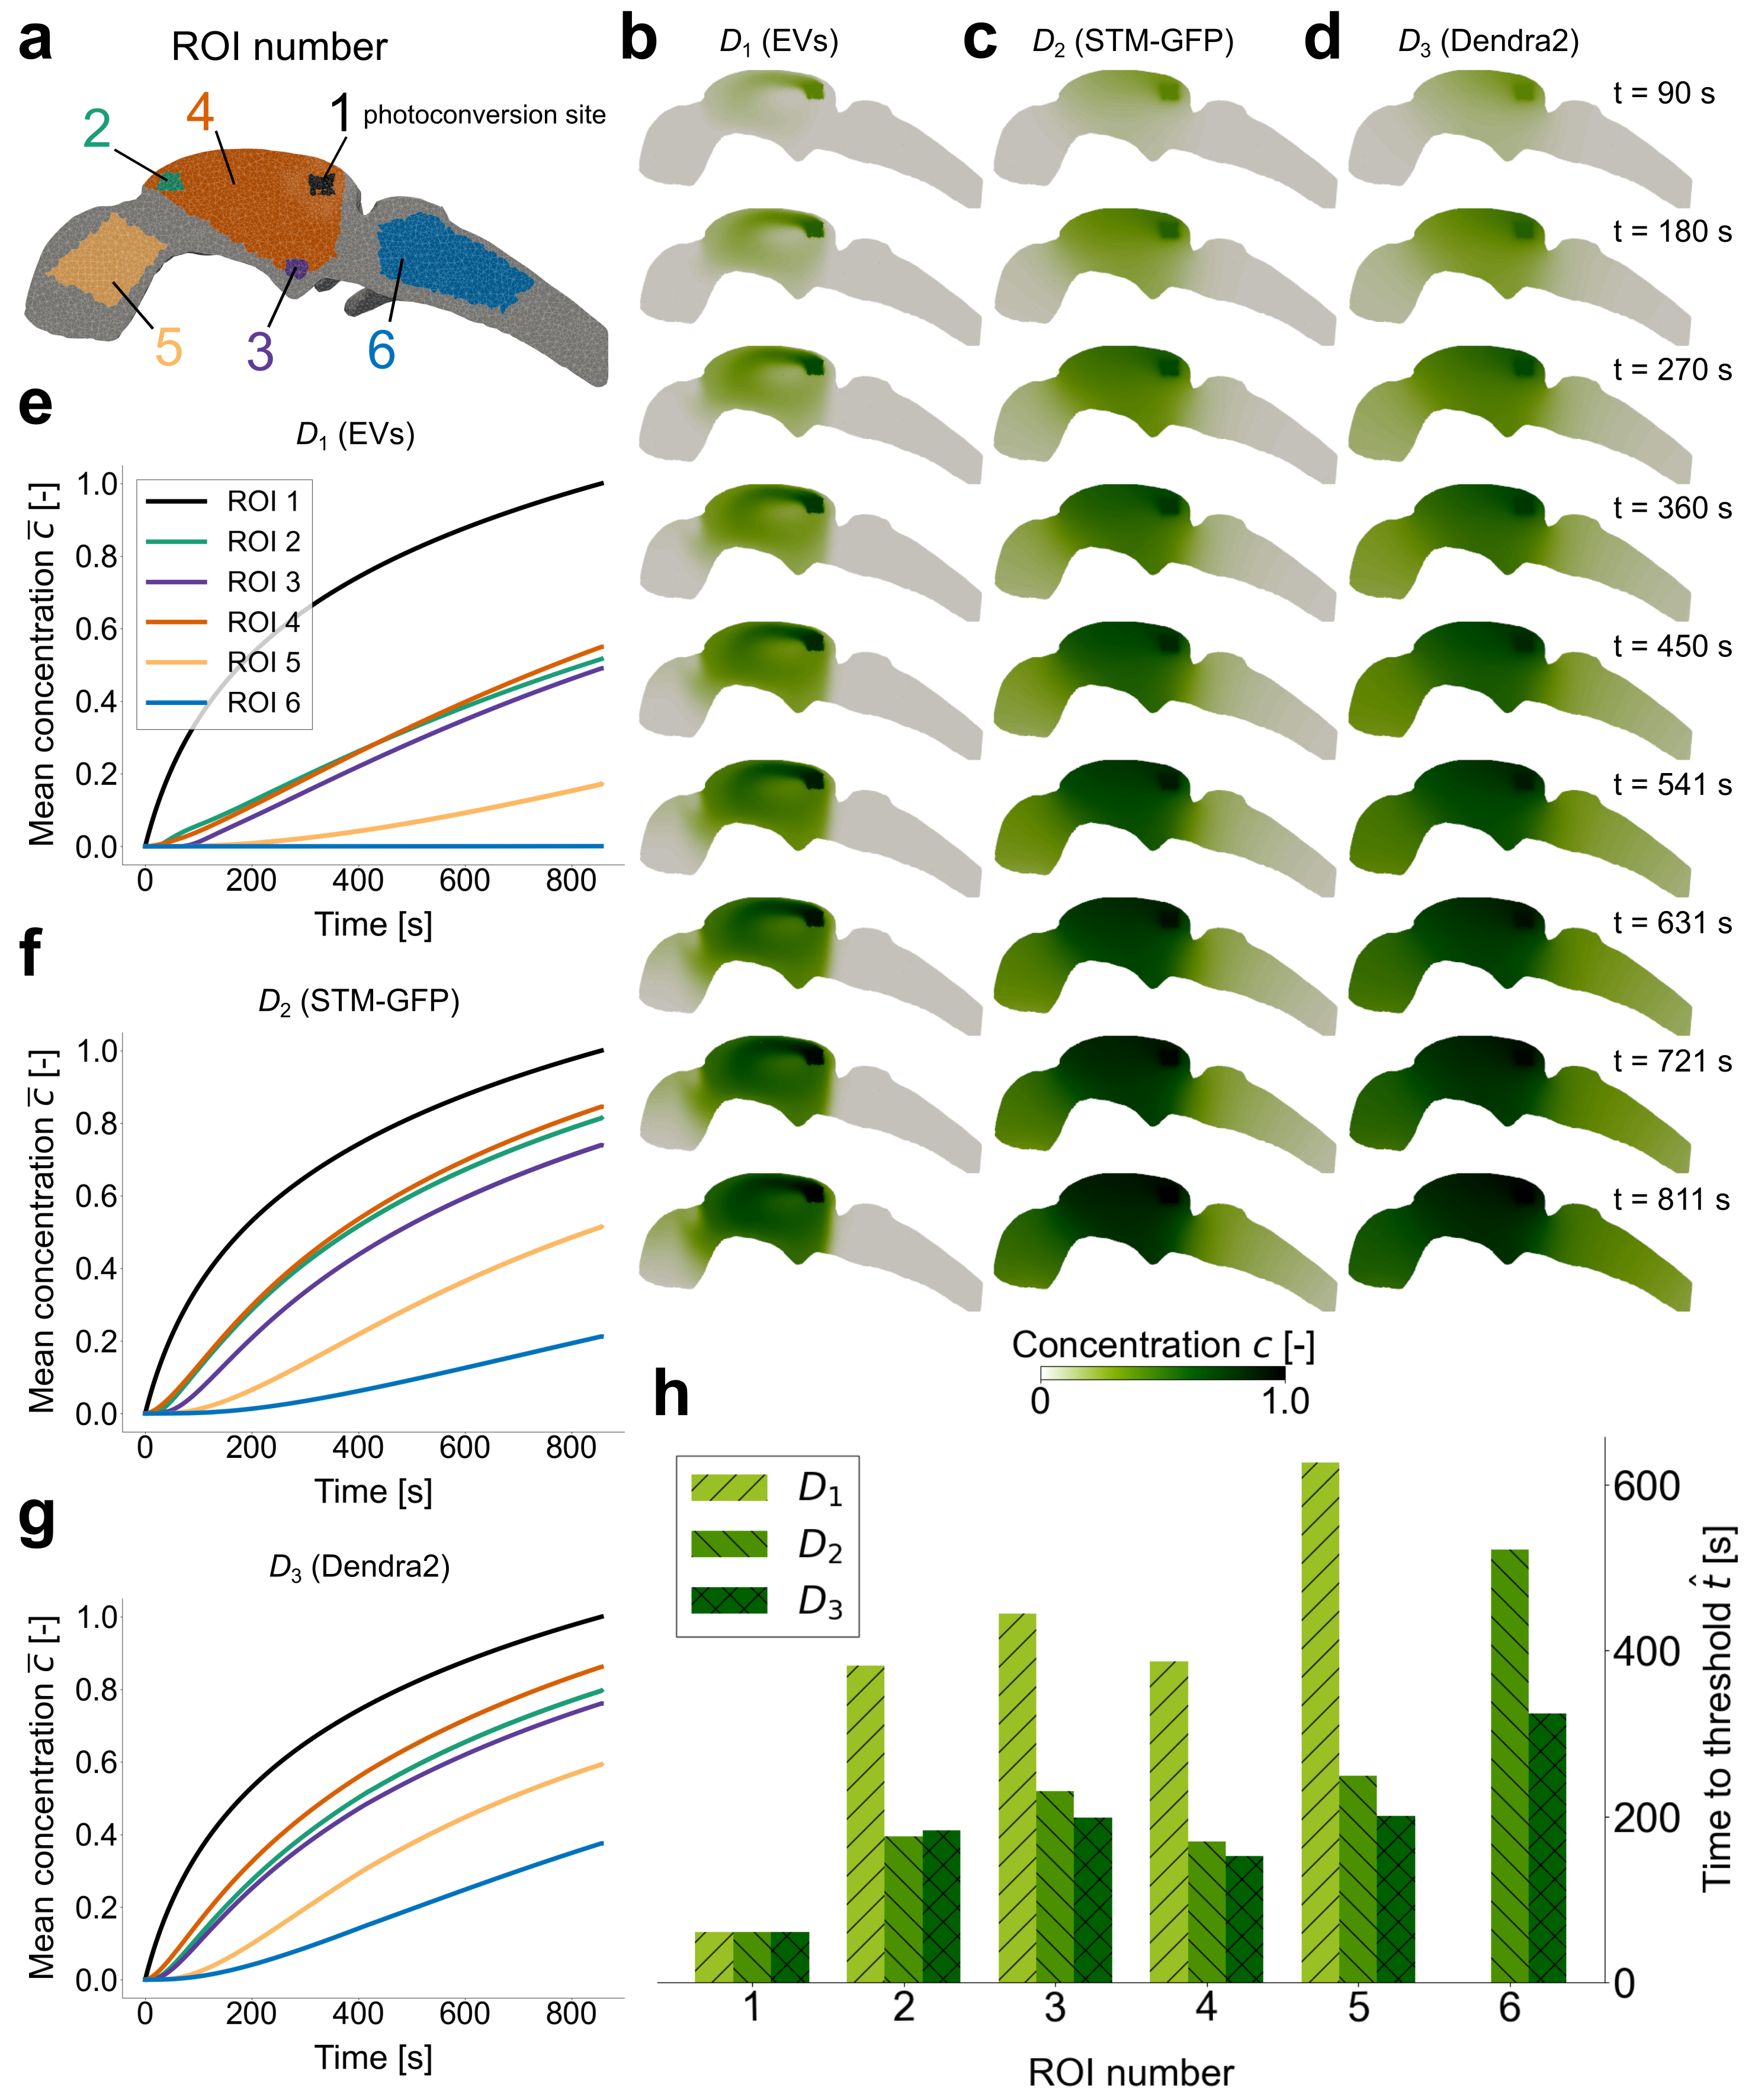
\includegraphics[width=\textwidth]{graphics/figure2_simulation_results_different_coeffs.png}
    \caption{Simulated distribution and evolution after photoconversion of
    extracellular vesicles (EVs, $D_1$), STM-GFP ($D_2$) and Dendra2 ($D_3$). 
    \textbf{a.} Geometry-centered clip of the ventricles mesh showing the locations of the 
    regions of interest (ROIs).
    \textbf{b--d.} Slices of the concentration field simulated
    with diffusion coefficients $D_1$, $D_2$ and $D_3$ for nine time instants covering the
    time range from 90 seconds to 811 seconds, corresponding to 200 to 1800 cardiac cycles,
    for even intervals of 200 cycles.
    Slices are taken in the $xz$-plane ($y=0.140$ mm, the center of the geometry).
    \textbf{e--g.} Mean concentration $\cbar$ in each ROI
    as function of time for diffusion coefficients $D_1$, $D_2$ and $D_3$. 
    \textbf{h.} The time $\hat{t}$ before the mean concentration $\cbar$ exceeds a
    threshold value of $0.25$ (ROIs 2-4) or $0.10$ (ROIs 5, 6) in each simulation setup.
    Note that there is no bar for $D_1$ in ROI 6, because the threshold value was never exceeded.}
    \label{fig:fig2}
\end{figure}

To further quantify the solute transport, we examine the mean
concentrations $\cbar_i(t)$ in six ROIs over time
(\Crefpanels{fig:fig2}{e--g}) and, in addition, the times $\hat{t}_i$
when the mean concentrations first exceed a threshold value
$\hat{c}_i$ (\Crefpanels{fig:fig2}{h}).  Higher diffusion coefficients
result in more rapid transport (\Crefpanels{fig:fig2}{e--g}), with
lower times-to-threshold in ROIs 2--6 (\Crefpanels{fig:fig2}{h}). For
all three diffusion coefficients, the solute first spreads within the
middle ventricle, covering ROIs 2--4, before appearing in the anterior
ventricle (ROI 5) and finally reaching the posterior ventricle
(ROI 6). Notably, the extracellular vesicles, associated with the smallest diffusion
coefficient, do not reach the posterior ventricle (ROI 6) within the
simulated time frame~\Crefpanels{fig:fig2}{b, e}.

\subsection{Model validation by comparison with photoconversion experiments}

To validate the model predictions, we performed photoconversion
experiments in transgenic zebrafish larvae expressing the secreted
Dendra2 in their brain ventricles. The approach is inspired by earlier work
where a photoconvertible protein was injected into the ventricle~\cite{fame2016directional}.
By using a transgenic system where the protein is directly secreted into the CSF,
we avoid detrimental effects of intraventricular injection on CSF properties. 
Our photoconversion protocol
consisted of the acquisition of a baseline fluorescence intensity
$F_0$, before localized exposure to a UV laser (at ROI 1) that
converts Dendra2 from a green- to a red-emitting fluorescent
protein. To quantify the transport of photoconverted proteins, we
measured and calculated the change in fluorescence intensity $\Delta F(t)
= (F(t)-F_0)/F_0$ over time (\Crefpanels{fig:fig3}{a}).

Comparison of the intensity changes with the simulated concentration
profiles in ROIs 1--6 (\Crefpanels{fig:fig3}{a, b}) shows that the
model predictions agree well with the experimental measurements. We
note minor differences however. The simulated values of $\cbar_i$ at
the final time (0.80, 0.76, 0.86, 0.60 and 0.38 in ROIs 2--6, respectively)
are generally higher than the corresponding experimental $\Delta F$
values (0.63, 0.71, 0.67, 0.29 and 0.18). Moreover, we observe
differences in the distribution within the middle ventricle,
especially with regard to ROIs 2 and 3. Overall, we note that the time
to reach a 25\% threshold agree well between the model predictions and
experimental values (\Crefpanels{fig:fig3}{c, d}).

\begin{figure}[H]
    \centering
    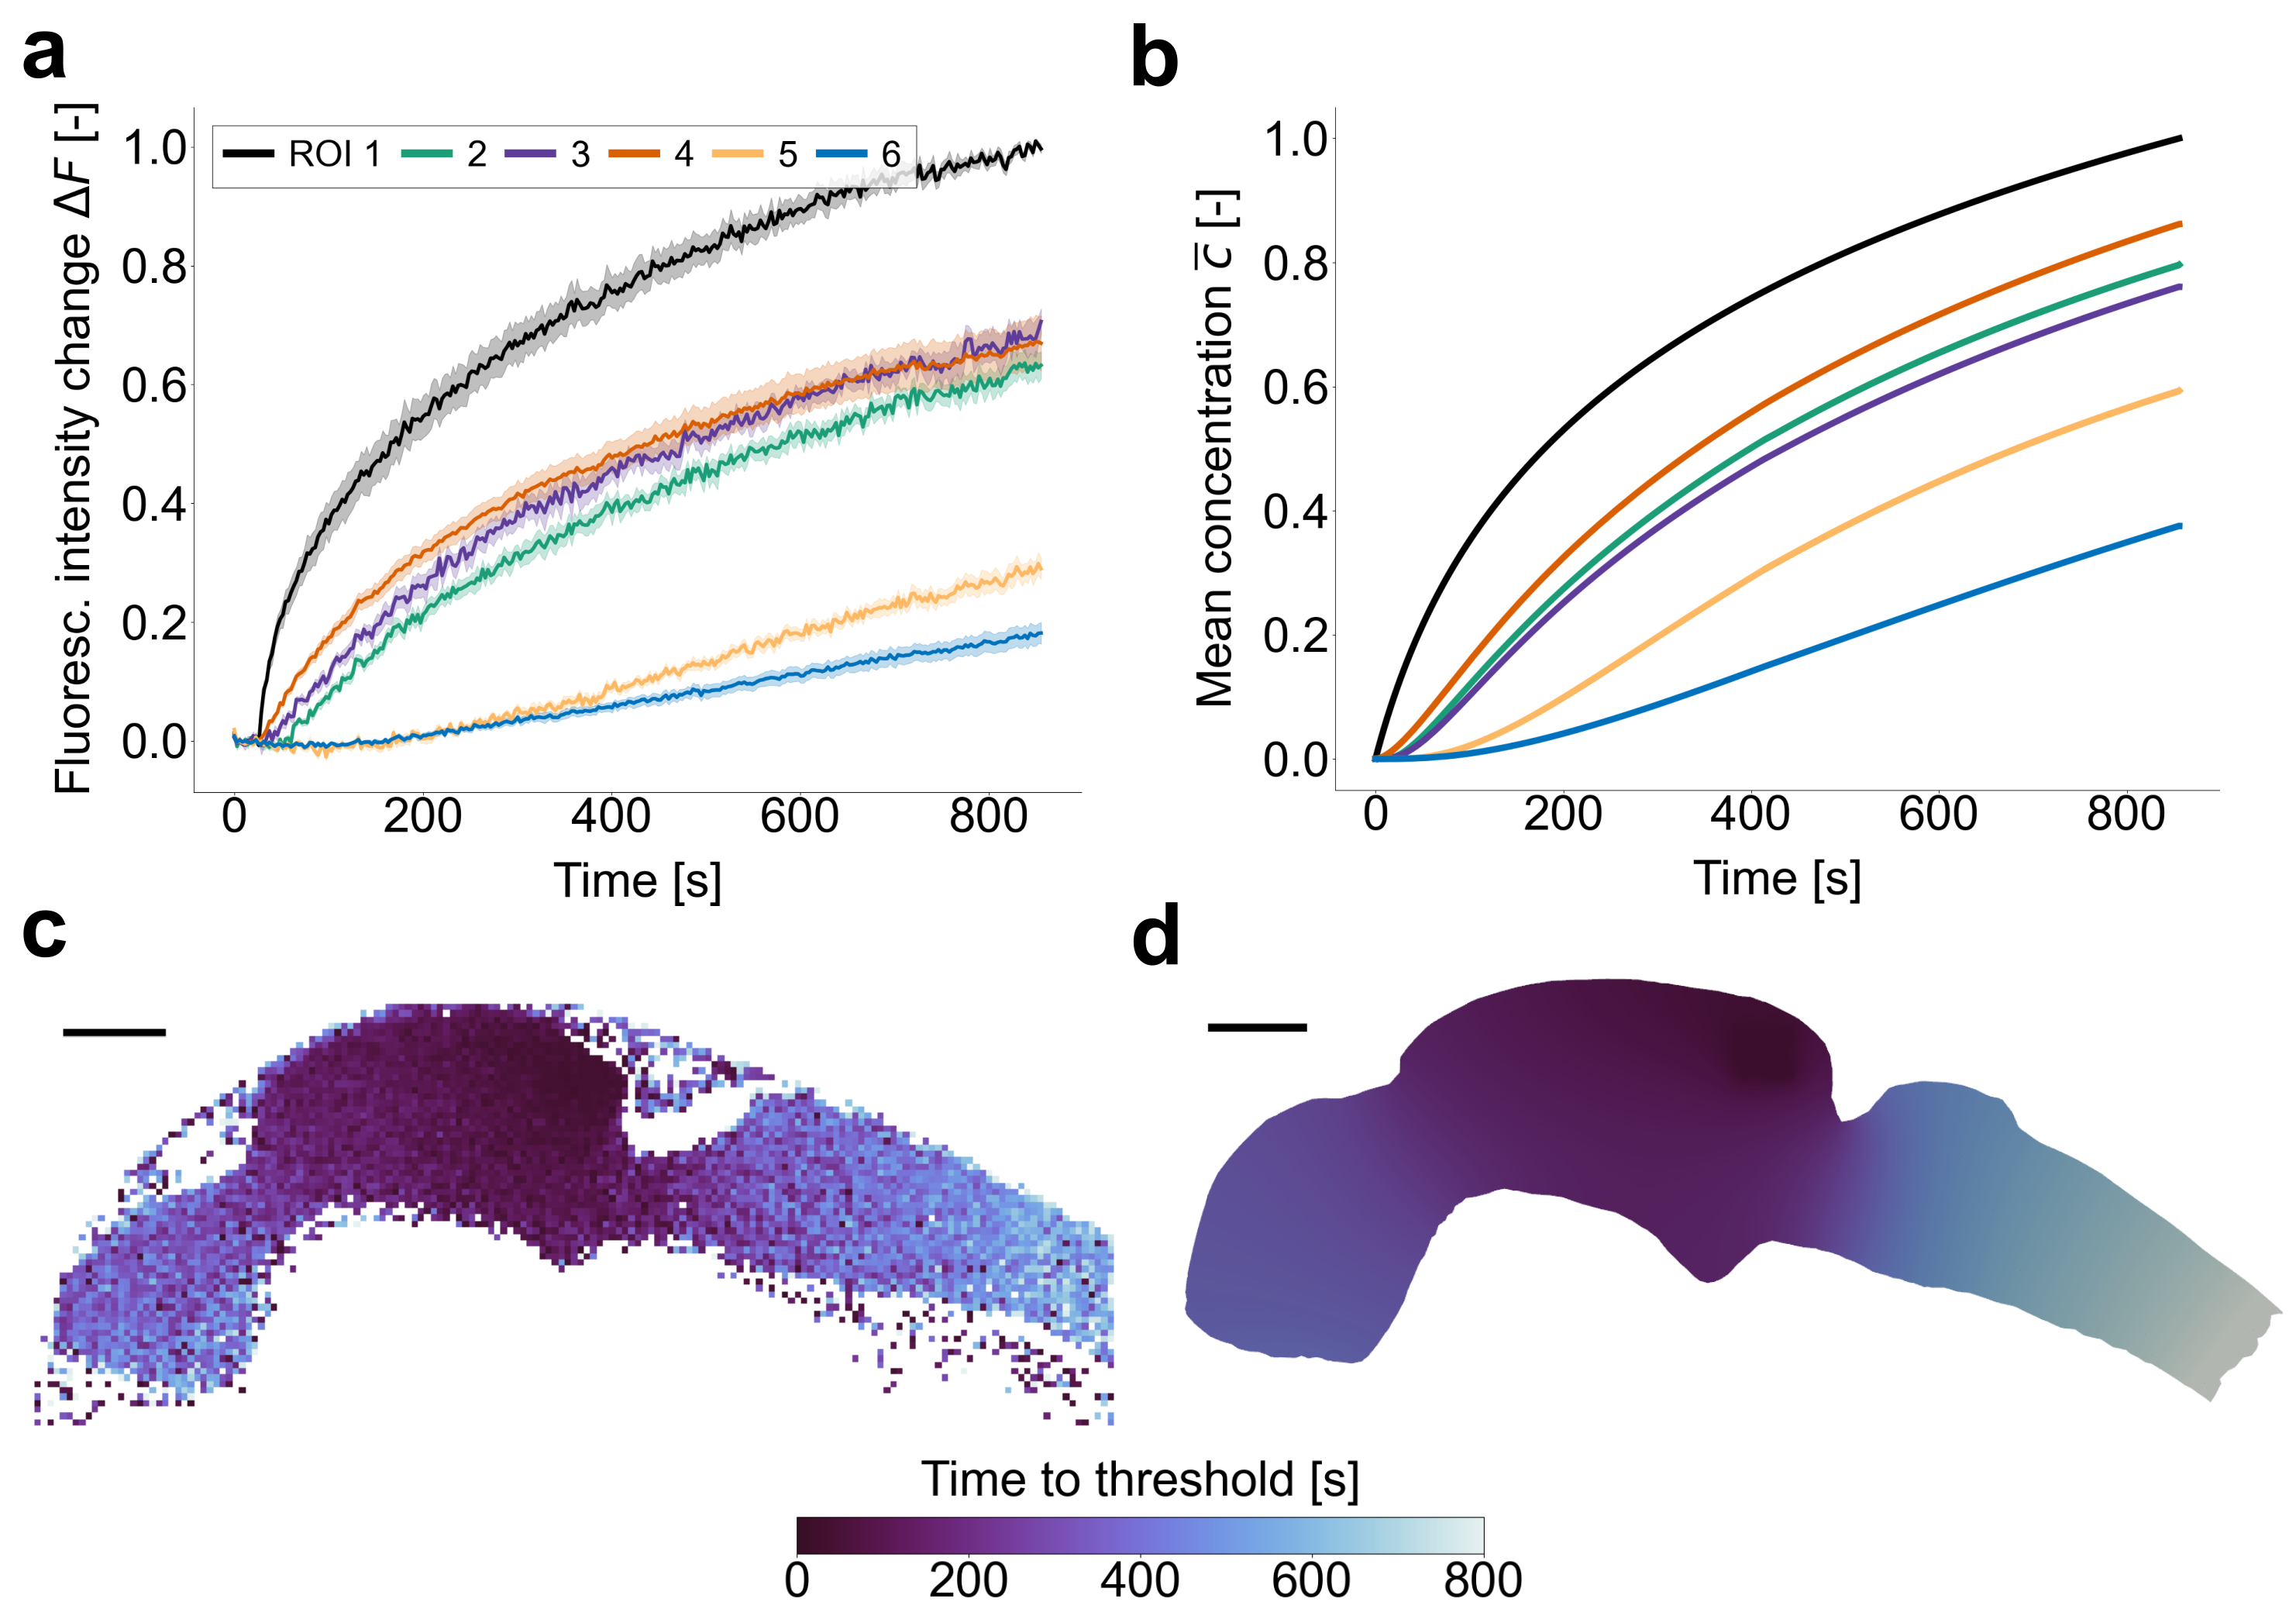
\includegraphics[width=0.975\textwidth]{graphics/figure3_compare_experiments_and_simulations.png}
    \caption{
    \textbf{a.} Relative change in fluorescence intensity $\Delta F(t)$ 
    in each region of interest (ROI)
    observed during experiments monitoring
    the movement of Dendra2 proteins photoconverted by laser targeting ROI 1. 
    Bold lines are mean values of the cohort ($n=8$) and shaded regions cover
    one standard devation errors in the mean.
    \textbf{b.} Mean concentration $\cbar(t)$ in each ROI in a
    simulation of Dendra2 protein transport with
    the diffusion coefficient $D_3$.
    \textbf{c.} Time to $\Delta F(t)$ reaches a threshold value of 0.25 in
    one representative zebrafish larva.
    \textbf{d.} Time to $\cbar(t)$ reaches a threshold value of 0.25 for
    a transport simulation with diffusion coefficient $D_3$.
    We have excluded the posterior-most regions of the geometries,
    because the values of $\Delta F$ and $\cbar$ never exceeded the threshold
    value of 0.25 in these regions. Scale bars 50 \textmu m.}
    \label{fig:fig3}
\end{figure}
% Final Delta F values
%0.6322650156762044 ROI 2
%0.7059449124175479 ROI 3
%0.6694500367160006 ROI 4
%0.28986700094045437 ROI 5
%0.18155055624229066 ROI 6
% Final mean c values ROIs 2-6: 0.80, 0.76, 0.86, 0.60 and 0.38

\subsection{Absence of ciliary motion affects local solute distribution}

Ciliary motion is integral to physiological CSF flow,
and absence of cilia has been associated with defective
brain development and various pathologies~\cite{Eichele2020Cilia-drivenVentricle,
Olstad2019CiliaryDevelopment, Faubel2016Cilia-basedVentricles,
Guirao2010CouplingCilia, Afzelius2004CiliaRelatedDiseases,
Sawamoto2006NewBrain, Yoshiba2014RolesSymmetry,
Hirokawa2006NodalAsymmetry}.
As observed both experimentally and computationally,
absence of motile cilia alters CSF flow patterns. 
We next investigate the implications of these changes on intraventricular
transport.

We experimentally measured the movement of proteins by monitoring
photoconverted Dendra2 signal in control zebrafish and 
motile-cilia mutant \emph{schmalhans} (\emph{smh}) zebrafish.
In ROIs 2 and 4, which quantify Dendra2 distribution
downstream of the photoconversion site, we observed a slower increase
of fluorescence intensity (\Crefpanels{fig:fig4}{a}). The mean times-to-threshold
in the \emph{smh} mutants were $45\%$ (ROI 2) and $25\%$ (ROI 4) higher
compared to controls (\Crefpanels{fig:fig4}{b}). We found no significant differences
between \emph{smh} mutants and controls
in the Dendra2 distribution in ROIs 3, 5, and 6.

The \emph{smh} mutants are mimicked in the computational model by
considering transport of Dendra2 with CSF flow driven by cardiac
pressure pulsations only, representing the absence of motile
cilia. Comparing the in silico mutants with transport predictions in
the presence of both cardiac pulsations and motile cilia, we observe
noticeably delayed dynamics in ROIs 2, 4 and 5, but little change for
ROIs 3 and 6 (\Crefpanels{fig:fig4}{c}).

Compared to experimental data, the difference between the control and
mutant scenarios was even greater for the simulations, with the
times-to-threshold in ROI 2 and 4 being 81\% and 28\% higher in the
absence of cilia-mediated flow. Moreover, the ROI 5 $\cbar$ profiles
for the two configurations in our computational model deviate,
which is not the case in the experiments. Altogether,
our findings identify that, for smaller proteins such as Dendra2,
diffusion plays an important role for
solute movement to regions upstream in the cilia-mediated flow fields or to
distant ventricles, while cilia affect the downstream mean concentrations.

\begin{figure}[H]
    \centering
    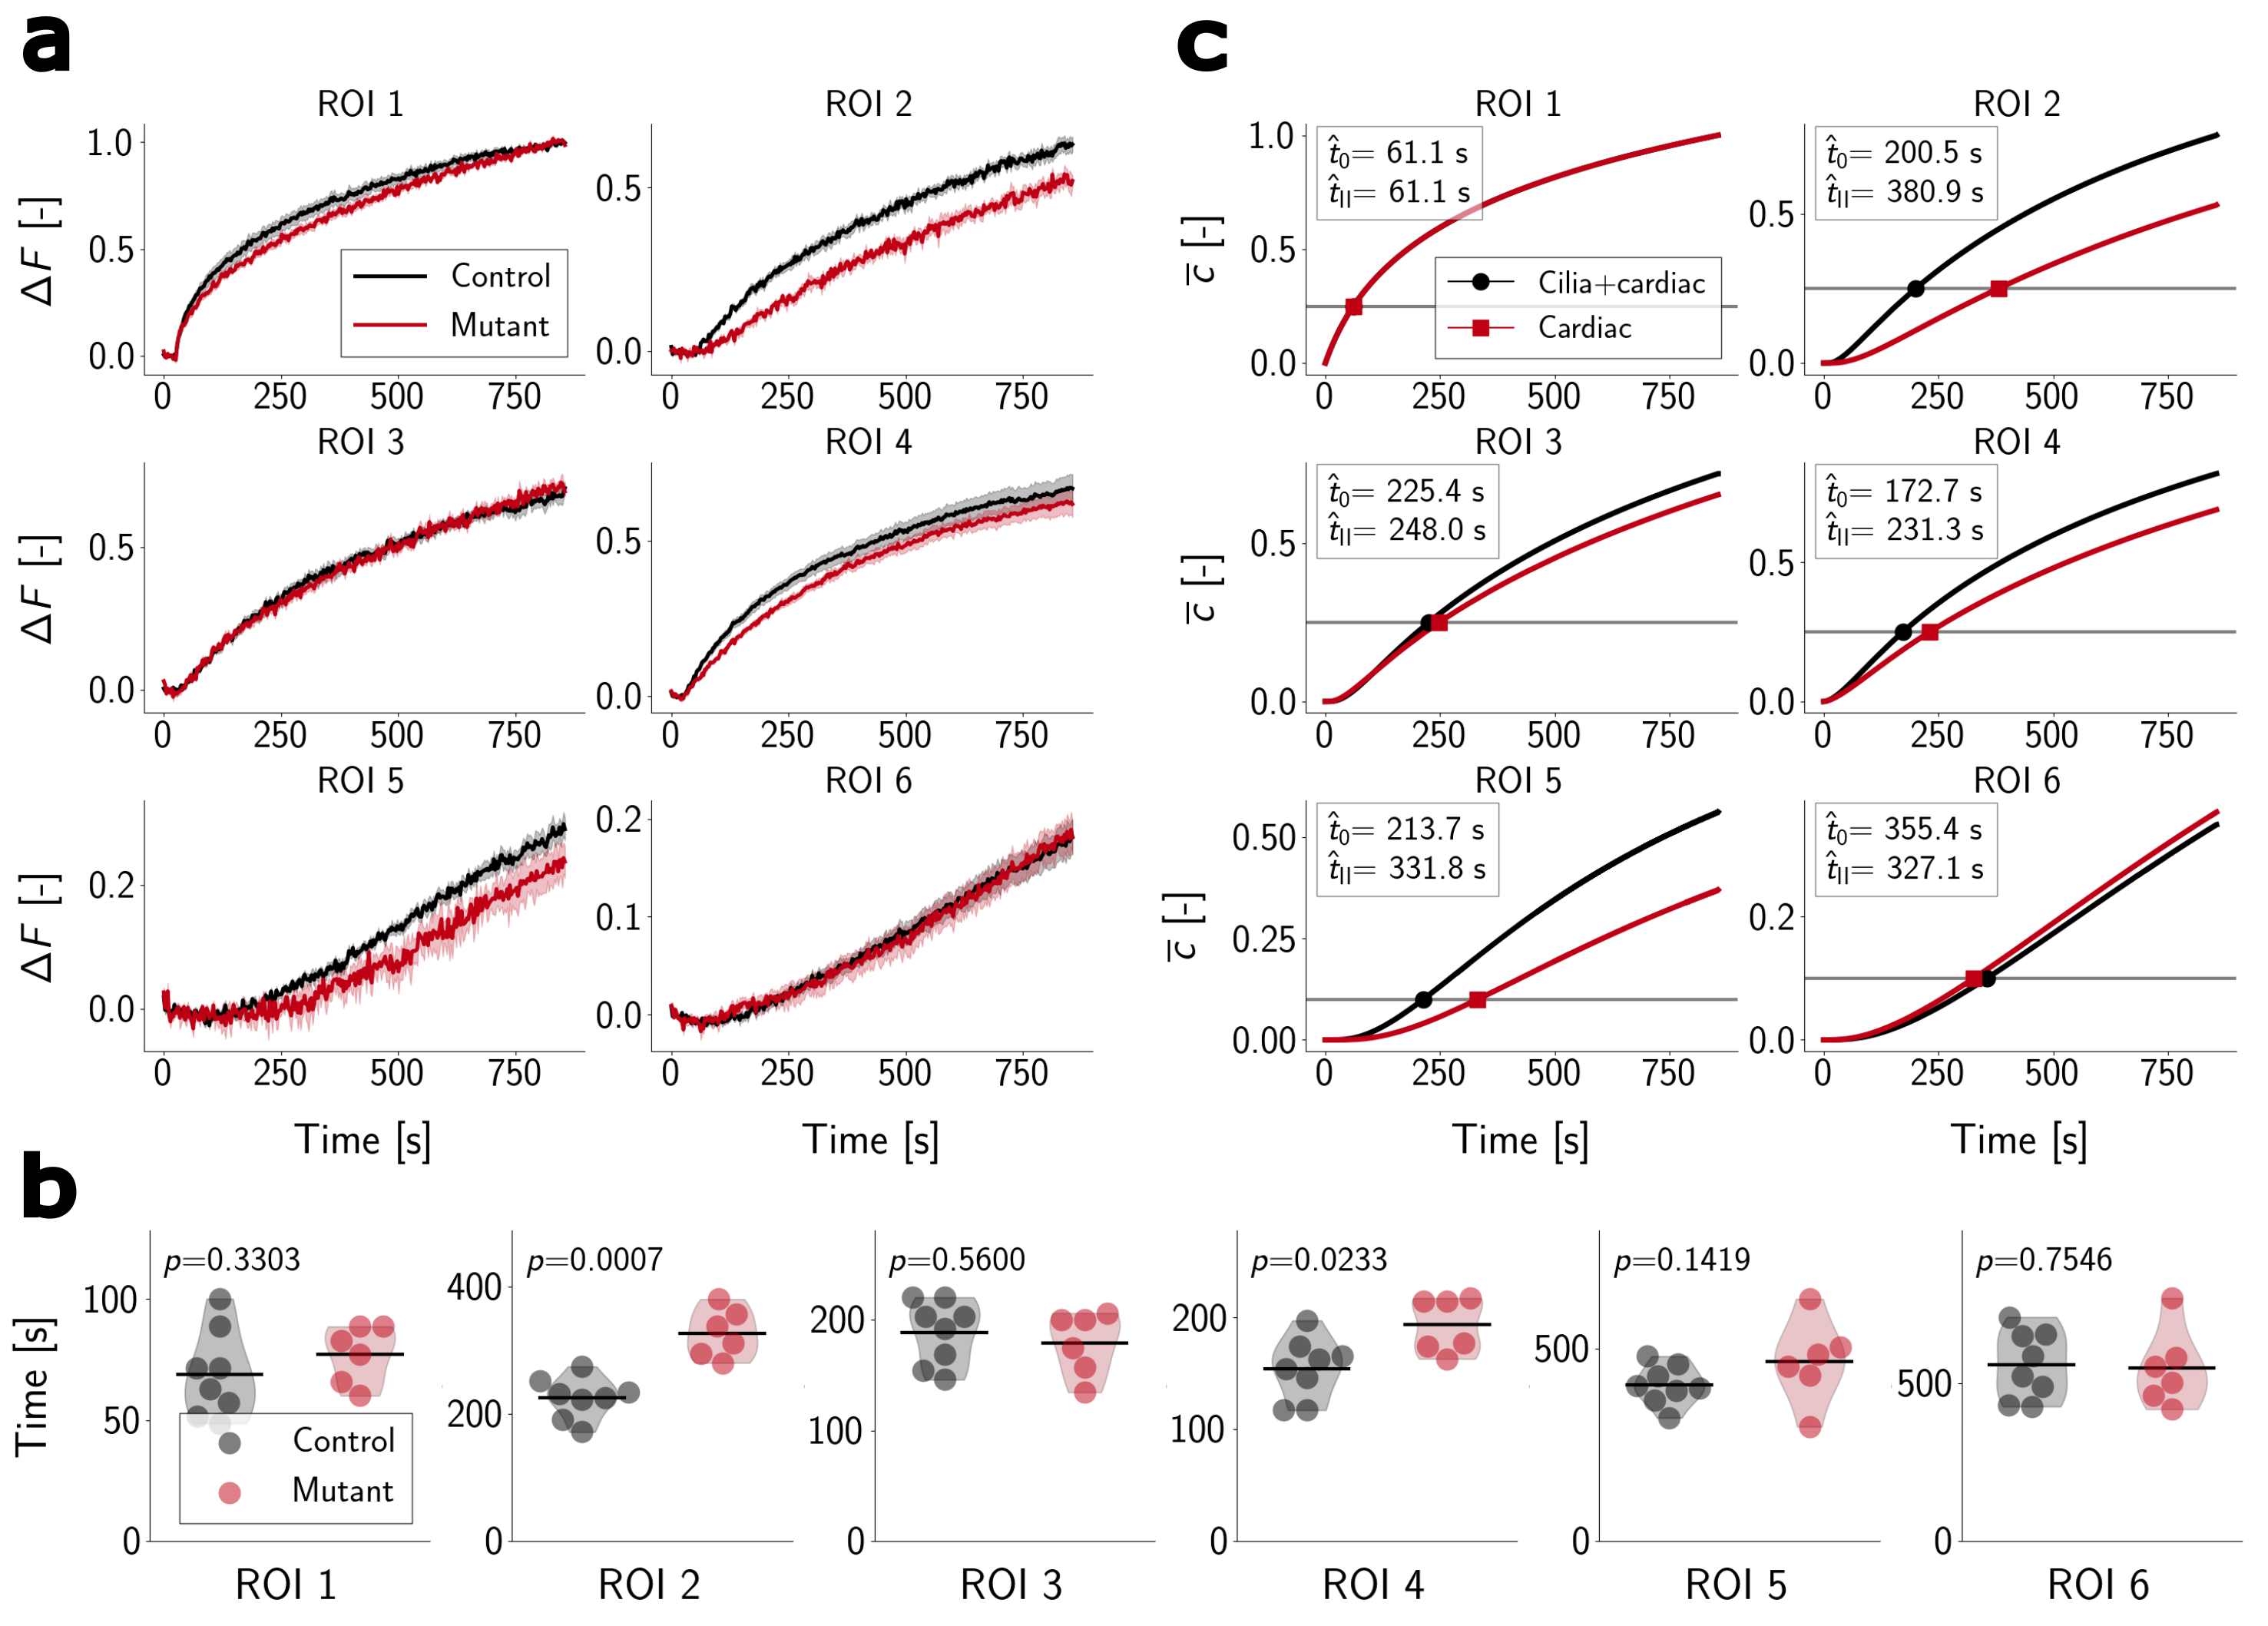
\includegraphics[width=\textwidth]{graphics/figure4_compare_control_mutant.png}
    \caption{\textbf{a.} Relative change in fluorescence intensity $\Delta F(t)$
    in each region of interest (ROI) for control (black lines, $n=8$)
    and \emph{smh} mutant (red lines, $n=6$) fish. 
    Bold lines are mean values of the cohorts and shaded regions cover one standard devation errors
    in the means.
    \textbf{b.} Times when $\Delta F(t)$ first exceeds a threshold value,
    equal to 0.25 (ROIs 2--4) or 0.10 (ROIs 5, 6), for control (gray dots) and
    \emph{smh} mutant (red dots) fish.
    The thick black lines denote mean values of the datasets. The $p$-values
    were calculated using a Mann-Whitney U test with a confidence level of 95\%, with 
    the null hypothesis that the two distributions of control and mutant data are 
    from the same population.
    \textbf{c.} Mean concentration $\cbar(t)$ in each ROI,
    simulated using the baseline model (black lines) and the cardiac-induced/no-cilia model (red lines).
    The horizontal gray lines mark the threshold value $\hat{c}$, and the time
    $\hat{t}$ when the threshold is first exceeded is reported in the plot legends.
    Note that in both panels \textbf{a} and \textbf{c}, the vertical axes have
    different limits in each plot.}
    \label{fig:fig4}
\end{figure}

\subsection{Loss of cilia motility in specific subpopulation slows down transport}

We previously characterized three distinct ciliated cell lineages in the
zebrafish larval brain~\cite{Olstad2019CiliaryDevelopment, DGama2025MotileBrain}.
To identify the effects of these lineages on CSF flow and transport, 
we investigate region-specific cilia paralysis with the computational model.
Three cilia-covered regions were considered paralyzed separately:
the anterior ventricle, and the dorsal and ventral parts
of the middle ventricle (\Crefpanels{fig:fig5}{a}).
To simulate cilia paralysis, the cilia tangential traction boundary condition
is for each case changed to a free-slip boundary condition
in the paralyzed region,
prescribing zero tangential forces to
represent absence of cilia motion.

The CSF velocities are most strongly
affected when removing cilia in the dorsal part of the middle ventricle,
as the maximum velocity magnitude drops from 27.9 \textmu m/s to 7.9 \textmu m/s.
In vivo, these dorsal cilia generate the strongest flow at
this developmental stage of the fish~(\Crefpanels{fig:fig1}{c})~\cite{Olstad2019CiliaryDevelopment}.
In contrast, removing cilia in the anterior ventricle or the ventral region of the middle
ventricle has minimal impact, and results in maximum speeds
of 27.9 \textmu m/s and 27.4 \textmu m/s, respectively.
Of the total tangential forces exerted by the cilia, ventral cilia in the middle ventricle
contribute with 34\%, while the dorsal cilia exert 52\% of the total tangential
force~(\Crefpanels{fig:fig5}{b}). The magnitude of these force contributions are thus
more similar than the difference in their impact on the maximum velocity magnitudes.
\begin{figure}[H]
    \centering
    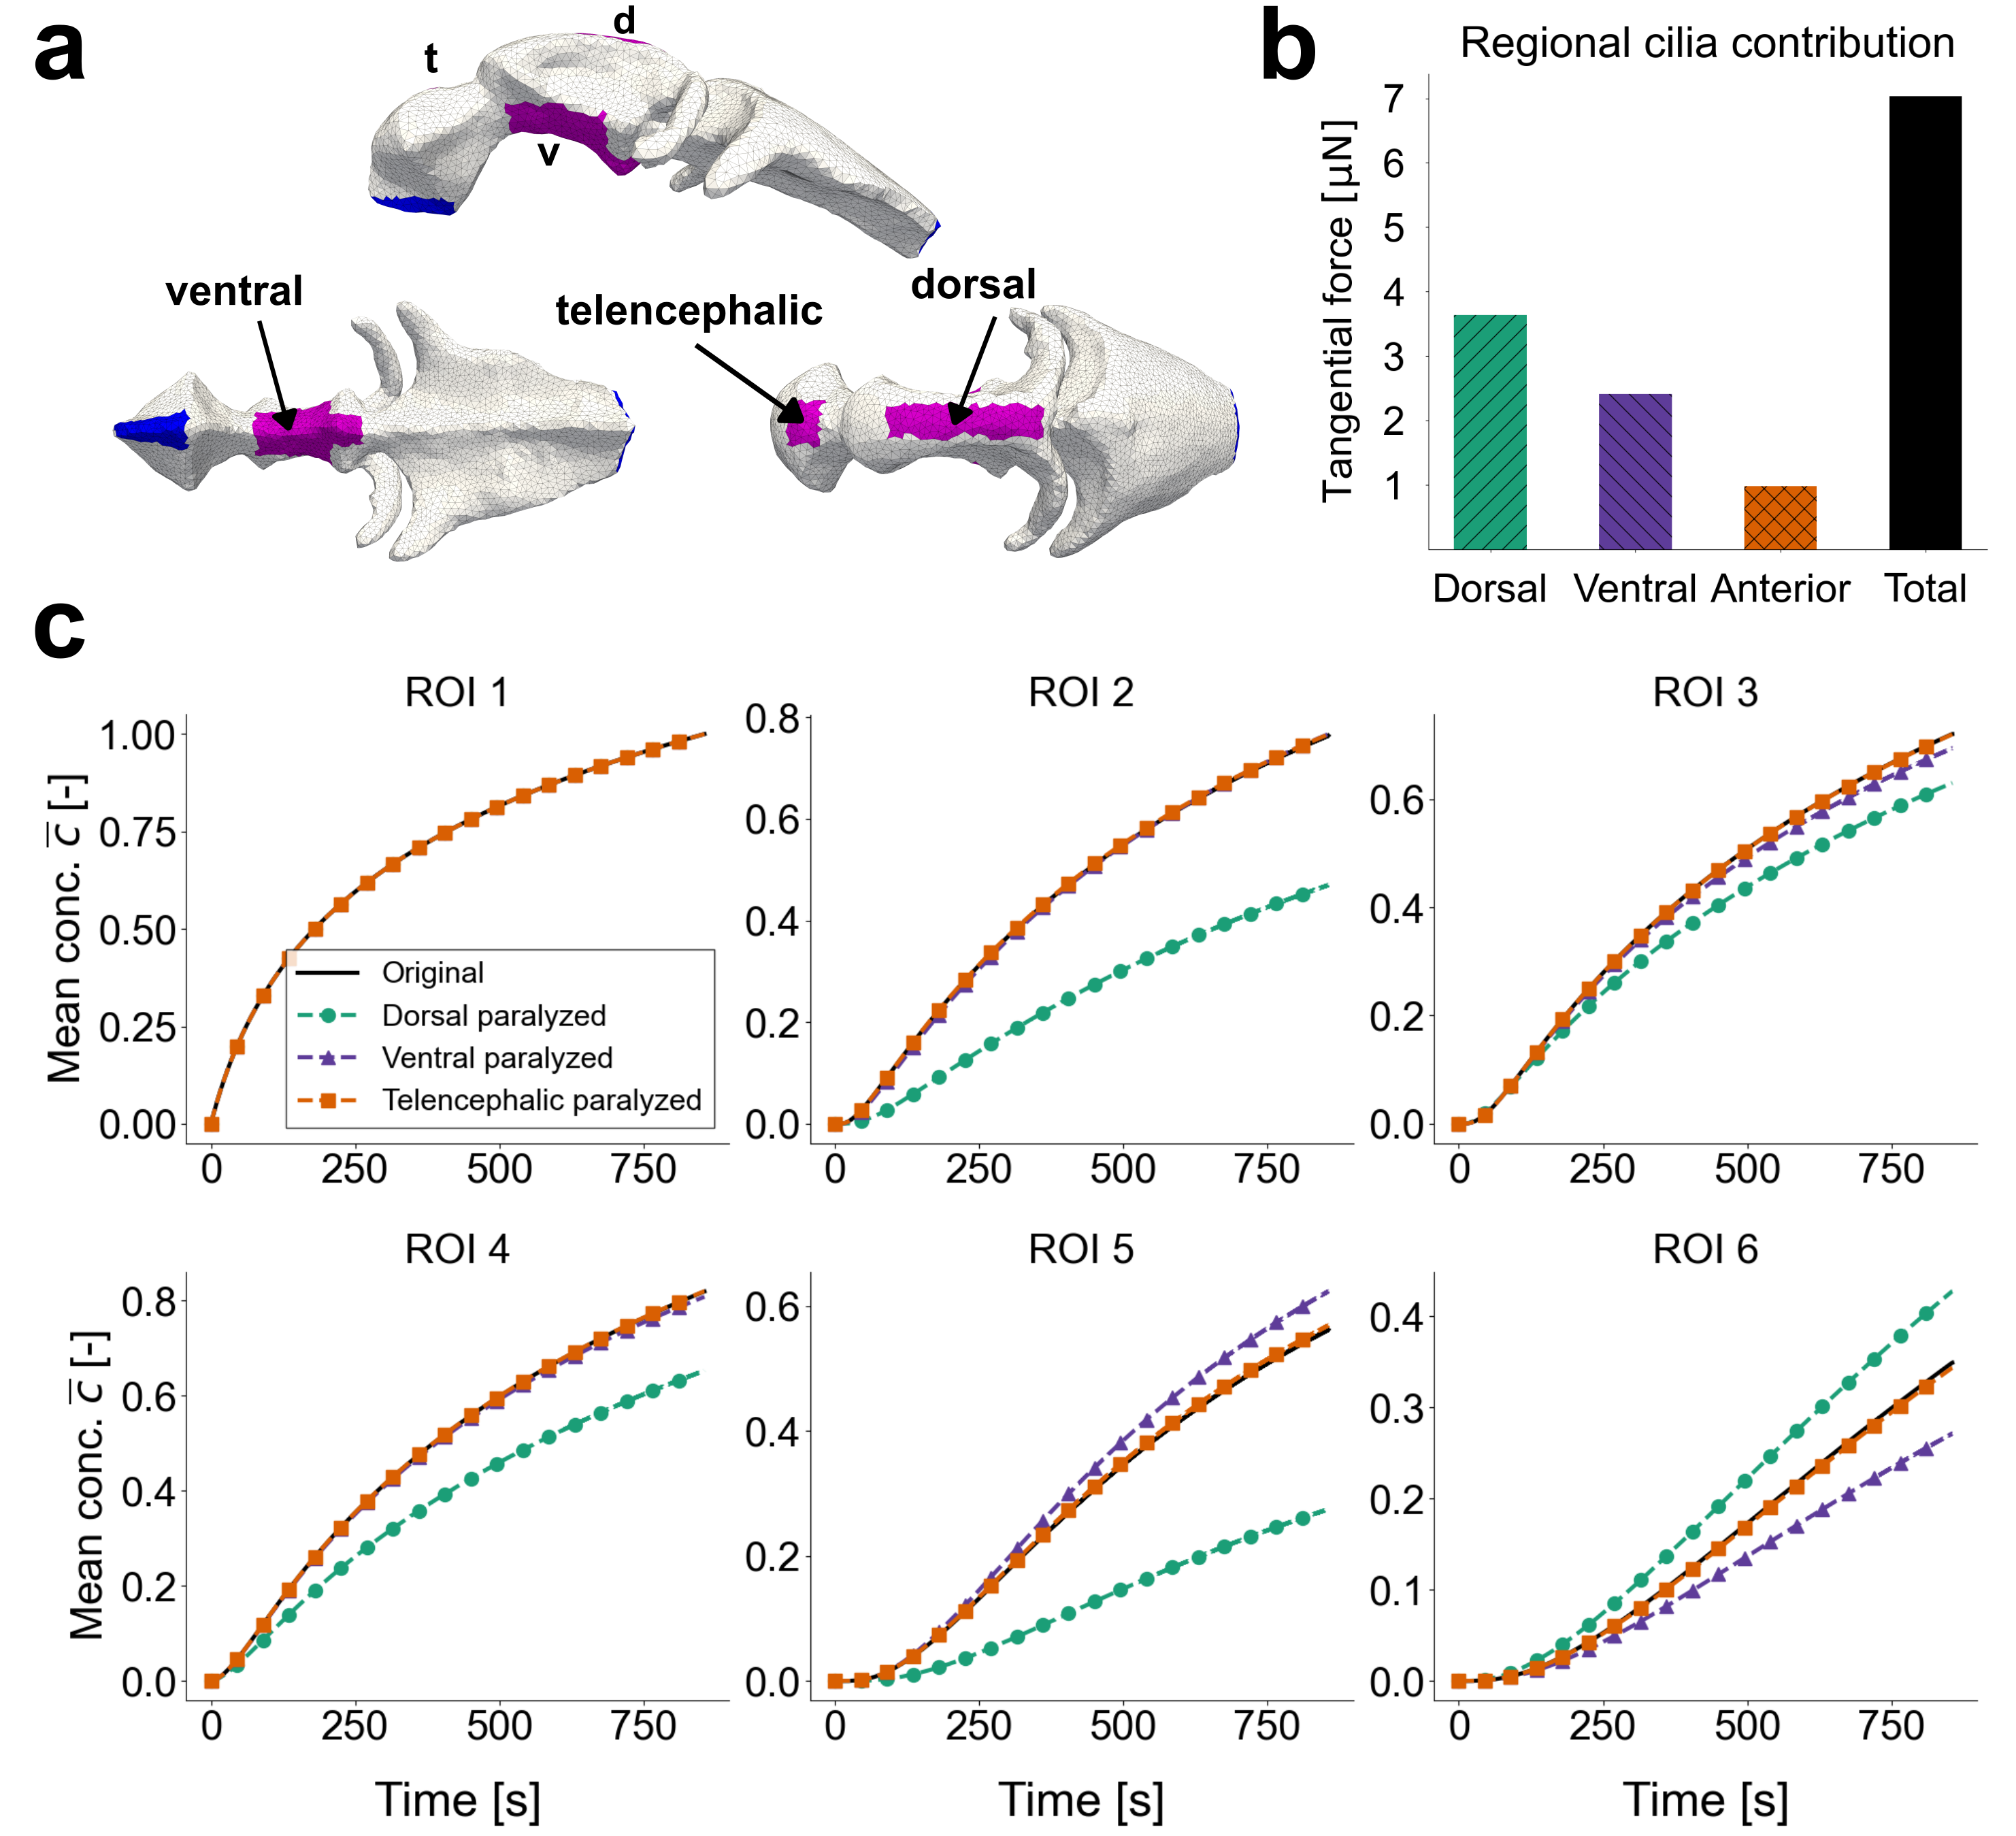
\includegraphics[width=\textwidth]{graphics/figure5_compare_cilia_modifications.png}
    \caption{\textbf{a.} The three separate cilia regions for which cilia paralysis is simulated
    by imposing a zero tangential traction boundary condition in the respective region.
    \textbf{b.} The total tangential force applied to the boundary with the tangential traction
    boundary condition in each of the three separate ciliated regions, as well as the total force
    (the sum of the three regions), calculated with \Cref{eq:tangential_force_calculation}. 
    \textbf{c.} Mean concentration $\cbar(t)$ for the six regions of interest (ROIs) in the three 
    paralysis scenarios considered. The region named in the legend is the region
    where we modify the cilia tangential traction boundary condition to a free-slip condition
    in the CSF flow model.}
    \label{fig:fig5}
\end{figure}

Changes in the transport of Dendra2 are most prominent when removing the dorsal cilia
in the middle ventricle. All mean concentration profiles 
(except ROI 1, where we impose the photoconversion curve)
exhibit changes (\Crefpanels{fig:fig5}{c}).
Compared to the baseline model results, we observe less solute distribution
in the middle and anterior ventricles (ROIs 2--5),
and more rapid transport to the posterior ventricle (ROI 6).
On the other hand, removal of anterior cilia does not alter the 
mean concentrations (\Crefpanels{fig:fig5}{c}).
Finally, without ventral cilia in the middle ventricle,
more solute spreads towards the anterior ventricle (ROI 5) and
less solute spreads towards the posterior ventricle (ROI 6).

\subsection{Modification of ventricular geometry impacts solute distribution}
Variations in ventricular morphology impact CSF flow patterns~\cite{Olstad2019CiliaryDevelopment}.
To assess how these variations influence solute distribution,
we consider four alternative ventricular geometries:
one where the duct connecting the anterior and middle ventricles is constricted
(66 \% reduction in cross-sectional area);
one where the duct connecting the middle and posterior ventricles is constricted
(33 \% reduction);
one where the middle ventricle is shrunk in the lateral direction (43 \% reduction);
and the combination of the above three modifications (\Crefpanels{fig:fig6}{a, b}).
In these four modified geometries, the total volume is reduced by
3.9\%, 4.1\%, 1.4\% and 9.4\%, respectively,
compared to the original geometry.

Constricting the connection between the anterior and middle ventricle reduces
solute transport to the anterior ventricle (ROI 5),
and the mean concentration in ROIs 2--4 and 6 slightly increases, compared to the original geometry
(\Crefpanels{fig:fig6}{c}). This is notwithstanding a
9.5\% reduction in ventral cilia force magnitude
(\Crefpanels{fig:fig6}{d}), which are the cilia that propel CSF and solute towards ROI 6.
Constricting the mid-hind brain connection
leads to less transport into the posterior ventricle (ROI 6),
and slightly more transport towards the anterior ventricle (ROI 5).
Faster transport to the anterior ventricle (ROI 5) and slower transport to the
posterior ventricle (ROI 6) is also the case for the geometry with a
shrunk middle ventricle.
This reduction in the transport to the posterior ventricle (ROI 6)
happens in spite of a 6.6\% increase in the ventral cilia forces.
Additionally, for the shrunk middle configuration, the transport upstream of CSF flow towards the
ventral-posterior region of the middle ventricle (ROI 3) is slowed down.

For the mesh where all three ventricles are modified,
we observe higher retention of solute in the middle ventricle (ROIs 2--4),
while both the anterior and the posterior ventricles (ROIs 5 and 6) have reduced
mean concentrations. To summarize, our results show that the
ventricular geometry and the cross-sectional area of the ventricular ducts matter
for solute transport, with notable differences in transport resulting from
relatively modest geometry modifications. This may explain why
we observed larger differences in the cilia-deficient computational
model results compared to the experimental data in \Cref{fig:fig4},
as the model and the fish have slightly different geometries.
\begin{figure}
    \centering
    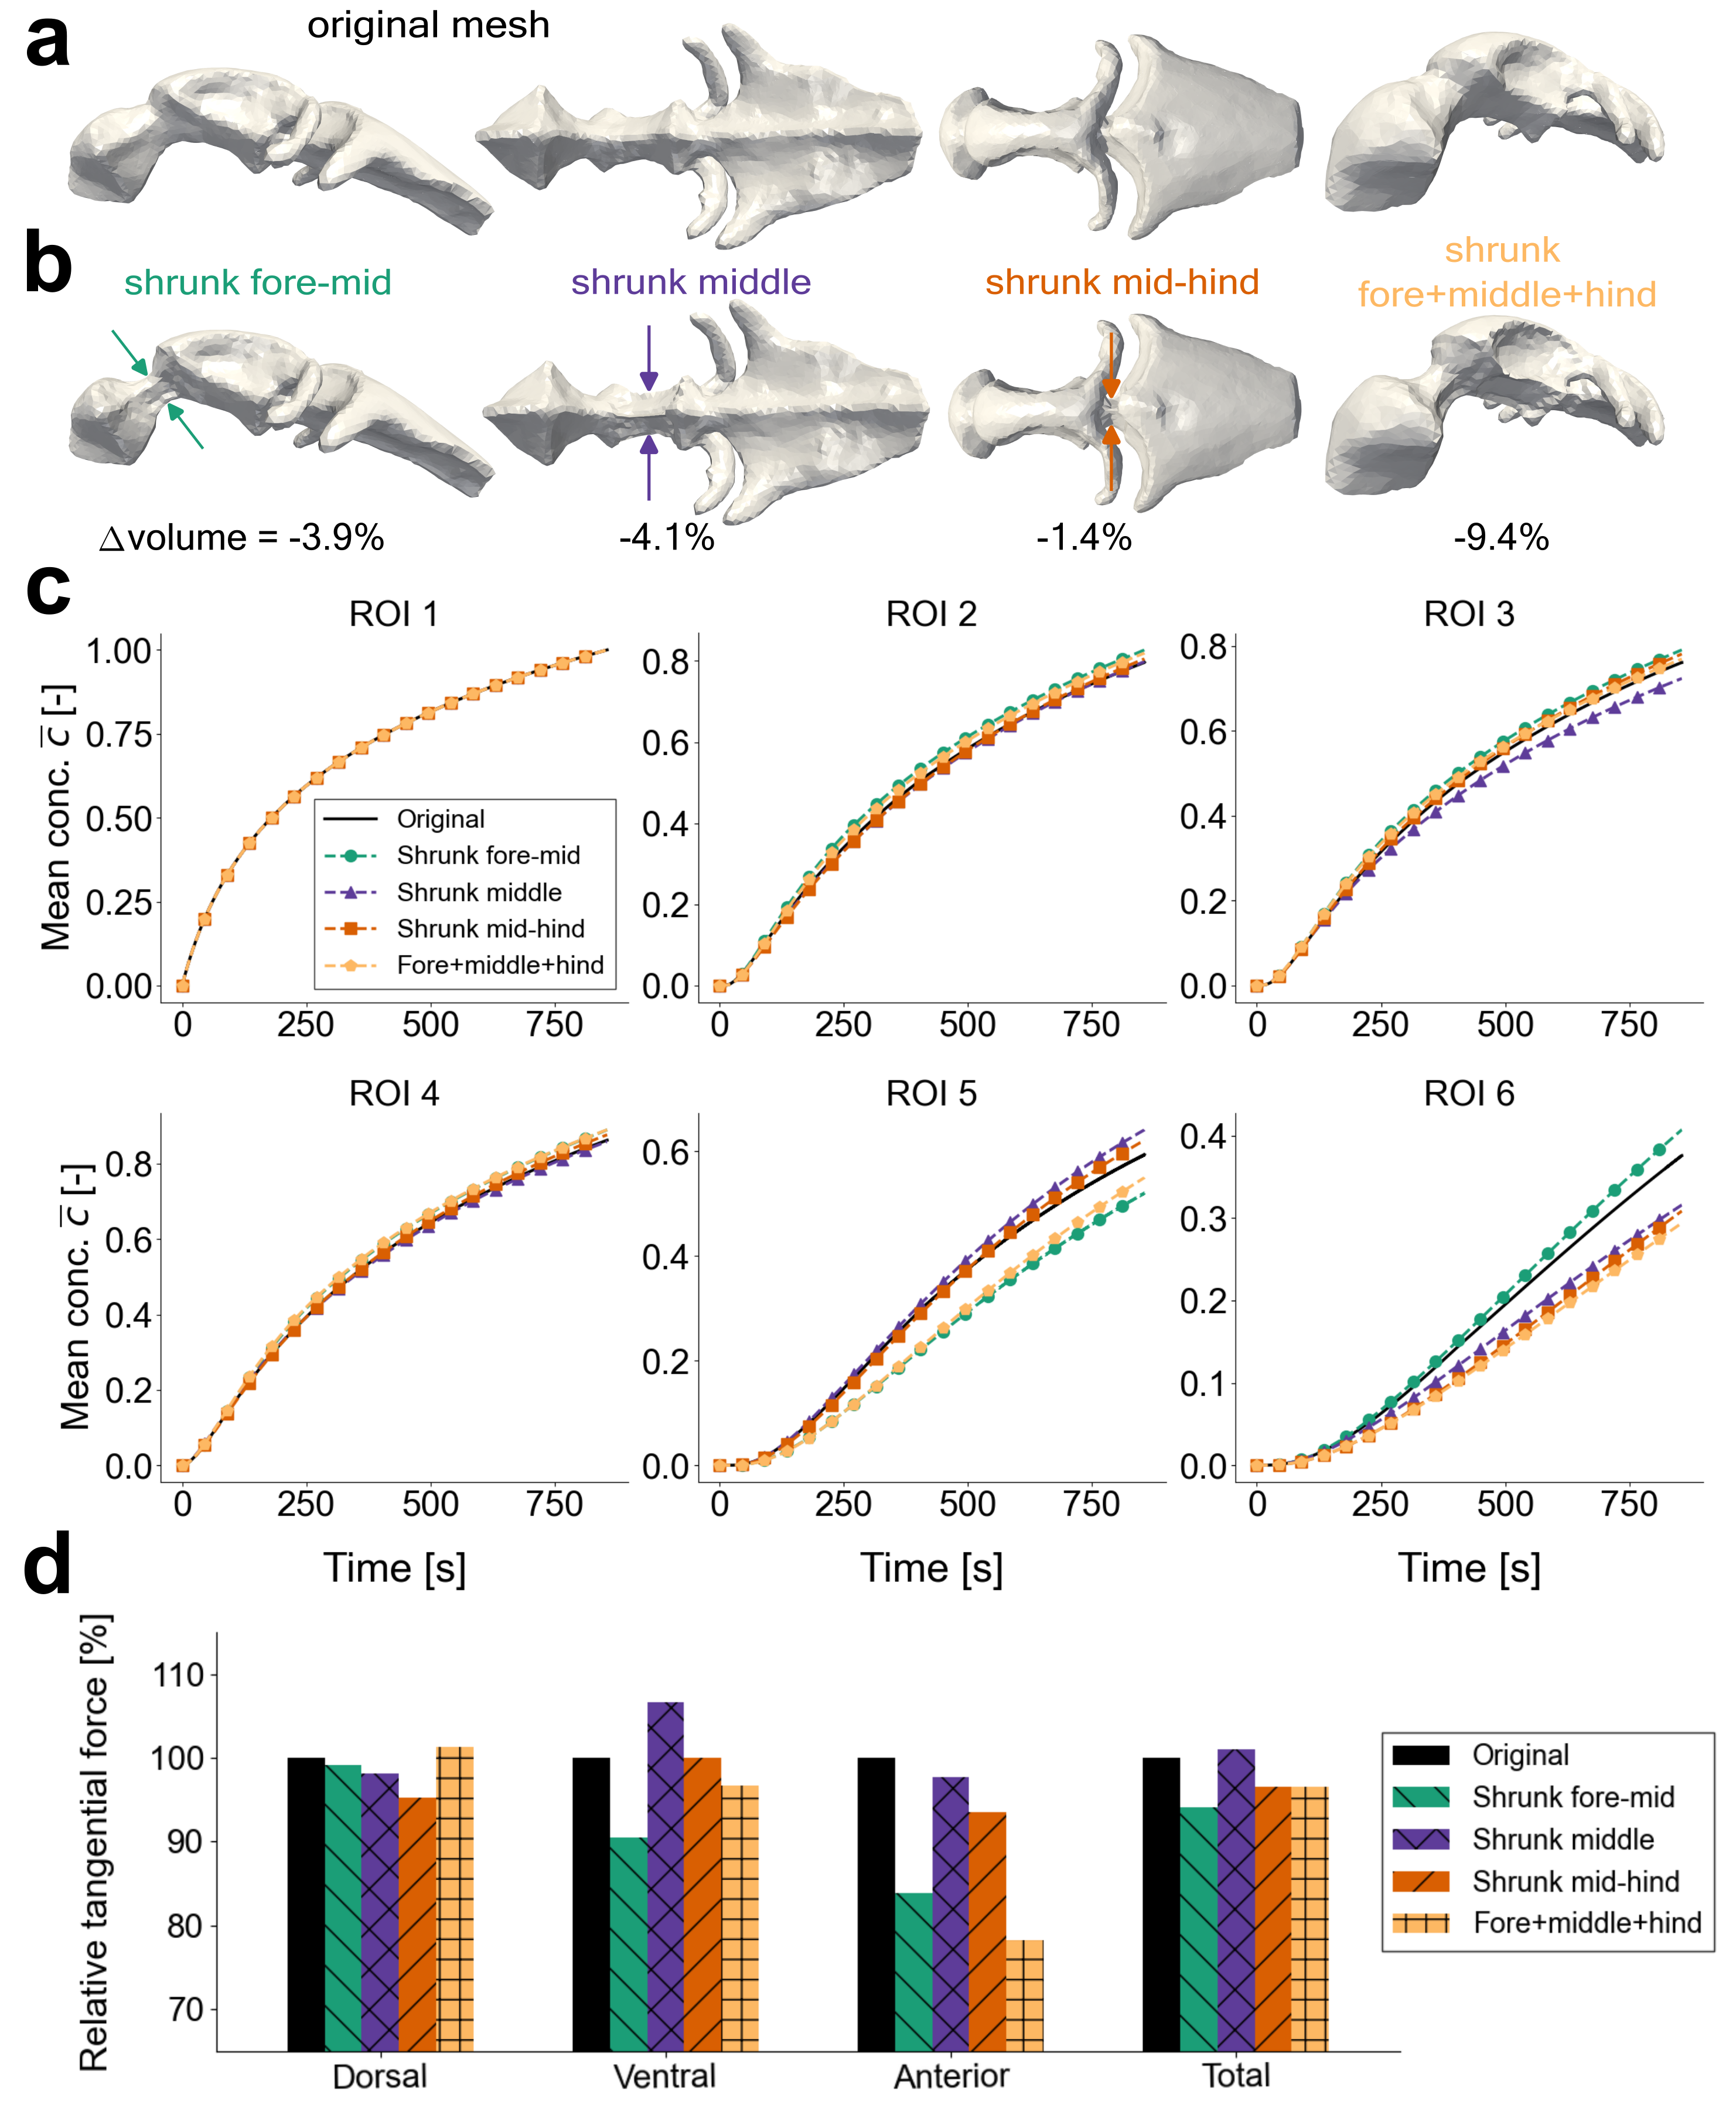
\includegraphics[width=\textwidth]{graphics/figure6_compare_modified_geometries.png}
    \caption{\textbf{a.} The original computational mesh of the ventricular geometry.
    \textbf{b.} The four modified versions of the computational geometry. Compared
    to the original mesh, the volumes of the deformed meshes are reduced by 3.9\%, 4.1\%, 1.4\% 
    and 9.4\%.
    \textbf{c.} Mean concentration $\cbar(t)$ simulated with the original and modified geometries
    in the 6 ROIs.
    \textbf{d.} A comparison of the tangential cilia force in the three cilia regions
    and the total force applied, calculated with \Cref{eq:tangential_force_calculation}.
    In each region, the force $F_{\mathrm{original}}$ 
    applied on the original mesh is the baseline of 100\%,
    to which the forces $F_i$ of the other mesh versions are compared, where $i$ denotes
    the cases fore-shrunk, middle shrunk, mid-hind shrunk, and the combination of the three.
    The bars for the four shrunk scenarios display $F_i/F_{\mathrm{original}}\times 100\%$.}
    \label{fig:fig6}
\end{figure}

\section{Discussion}
In this study, we have presented a computational model of CSF flow and
solute transport within the brain ventricles.
We used the larval zebrafish brain ventricles since its geometry and
flow mechanisms are well described, thereby allowing us to validate
our simulations experimentally. Nevertheless, our computational framework can be adapted to,
and implemented in, other ventricular systems in the future, once the flow parameters of such systems
are comprehensively resolved. We assumed that intraventricular CSF flow was governed
by the Stokes equations.
By imposing tangential traction and normal pressure
on the CSF flow, we were able to reproduce flow fields with similar features
as observed experimentally. The prominent flow features were vortex-structured flow,
mediated by cilia, and pulsatile flow, mediated by the cardiac cycle.

Using the simulated CSF flow, we modeled solute transport by an advection-diffusion equation.
The transport results compared well with data from in vivo experiments in zebrafish.
Then, by using a computational model as well as zebrafish mutants with paralyzed cilia,
we identified that even though advection by cilia is dominant,
diffusion plays a significant role in protein transport.
Finally, we investigated how local cilia paralysis and ventricular geometries
affect solute distribution. Altogether, we present not only new findings on the role of
diffusion and advection in intraventricular transport, but also provide a novel framework to
study CSF flow and transport in complex geometries.

\subsection{The roles of advection and diffusion in intraventricular solute transport}
To investigate the roles of advection and diffusion in solute transport, we quantified transport
based on changes in fluorescence intensity $\Delta F$ (experiments) and
mean concentration $\cbar$ (simulations) over time.
Even though we identified similar dynamics in simulations and
in vivo experiments, the dynamics of the simulations were generally
more rapid and resulted in higher total amounts of solute.
Differences between experiments and simulations may relate to
ventricular size, as we showed that modifying the geometry of the interventricular ducts
impacts solute distribution, and the geometry used for the computational model was larger
than some of the geometries used in experiments.
Notably, there are large variations in ventricular size in the control population at 2 dpf.
Alternatively, dissimilarities in results may relate
to the way we defined the photoconversion site (ROI 1) in the simulations,
since the volume of the photoconversion region determines
the total amount of solute and thereby the rate of transport. Another source
of discrepancy may relate to the permeability of the ventricular wall,
which we have ignored in our simulation. Reports have shown that the
neuroepithelium lining the walls of brain ventricles in 24 hour old zebrafish
is permeable to dyes smaller than 70 kDa~\cite{Chang2012AnNeuroepithelium}.
Since Dendra2 is around 26 kDa in size~\cite{Gurskaya2006EngineeringLight} and
thus under this reported limit, one could assume that Dendra2 may
leak out of the brain ventricles over the time spans we consider
and render the dynamics slower. Finally, an important difference
between the simulations and experiments is the fact that the
computational model is three-dimensional, while the
experiments only resolve two-dimensional features.

Nevertheless, our results convincingly show that
intraventricular transport of proteins depends on a balance of advection and diffusion.
While advection is the strongest transport mechanism on a global scale for
Dendra2 (global Péclet number 13), diffusion is balancing out
advection especially for shorter distances and for regions devoid of motile cilia activity.
Indeed, we identified that the diffusion coefficient had a greater impact on transport to
regions located upstream in the CSF flow field (ROI 3) or in distant ventricles (ROIs 5--6),
than the regions located downstream of cilia-mediated flow (ROI 2). 

Meanwhile, we identified that transport of larger molecules
(thus with smaller diffusion coefficients),
such as 150 nm radius extracellular vesicles, are almost entirely dependent on advection.
There was essentially zero solute in the posterior ventricle at the
final simulation time (around 860 s), a ventricle where transport is driven
by diffusion due to the absence of motile cilia.
For $D_1$, an estimate of the diffusion timescale $t_d=L^2/D_1$ over a distance
$L=200$ \textmu m from the middle to the posterior ventricle is approximately 24500 s.
Advective transport by the mean velocity $\overline{U}=2.4$ \textmu m/s over the same
distance would happen on a timescale of $t_a=L/\overline{U}=83$ s.
Comparing this with the minuscule values of $\cbar_6$ after simulating transport
with $D_1$ for 850 s, one can conclude that if advection
played a role in transporting solute from the photoconversion site in the middle ventricle
to the posterior ventricle, values of $\cbar_6$ would be higher than those observed.

\subsection{Effects of cilia motility and ventricular morphology}
To gain insights into how CSF flow and intraventricular transport depend on cilia
motility and ventricular morphology, we manipulated certain
parameters in our model and the computational geometry.
First, we investigated how complete loss of cilia motility
impacted the transport dynamics. Simulations with a cardiac-induced/no-cilia lead to
slower transport when compared to the baseline model that included cilia. Especially
the middle-ventricular region downstream of CSF flow (ROI 2) and the anterior ventricle (ROI 5)
experienced substantially increased times-to-threshold. We also observed
slower dynamics in the rest of the middle ventricle (ROIs 3 and 4), whereas the
posterior ventricle (ROI 6) was unaffected by the loss of cilia motility,
further indicating that transport from the middle to the posterior ventricle is
purely driven by diffusion at this developmental stage.
We also performed photoconversion experiments on cilia mutant
zebrafish larva (\emph{smh}), observing statistically significant slower transport in 
ROIs 2 and 4. The results provide not only confidence in that our computational model
represents the physics well, but also valuable quantification of the impact of cilia motility
on intraventricular transport. Interestingly, a previous simulation study of reduced cilia motility
also observed a drastic reduction in CSF mixing in specific regions of the brain
ventricles~\cite{Yoshida2022EffectVentricles}, similar to our results. Since impaired brain 
clearance of tracers has been demonstrated in idiopathic normal pressure hydrocephalus
patients~\cite{Eide2020MagneticHydrocephalus}, cilia-enhanced mixing in the brain might be
fundamental to physiological transport within the brain.

Next, we paralyzed cilia in specific regions of
our model. We identified that the cilia in the dorsal middle ventricle contribute
the most to solute distribution, which aligns well with the fact
that these cilia generate the strongest flow field in vivo~\cite{Olstad2019CiliaryDevelopment}
and in our model. In contrast, removing the ventral cilia in the middle ventricle
did not greatly impact flow dynamics, despite these cilia contributing a third of
the total force exerted by the cilia. However, removing ventral cilia in the middle ventricle
lead to reduced transport towards the posterior ventricle,
meanwhile increasing transport towards the anterior ventricle,
as the ventral cilia help induce flow towards the posterior ventricle.
Removing the cilia in the anterior ventricle affected CSF flow only locally,
and did not affect the global transport.

With an interest in assessing the impact of ventricular morphology on solute transport,
we simulated transport in modified ventricular geometries.
Notably, shrinking ducts reduced interventricular solute distribution, while shrinking
the middle ventricle obstructed diffusive transport upstream of the flow field.
We previously identified large interindividual variation in ventricular size and
CSF velocities between larva at given developmental stages and throughout
development~\cite{Olstad2019CiliaryDevelopment, DGama2025MotileBrain, Jeong2024TheZebrafish}.
Our results suggest that these two parameters, CSF velocities and ventricular size,
may well affect each other, which helps explain the variation in the two.

These simulation studies demonstrate that our model is flexible and allows in silico
testing of further hypotheses on the effects of ciliated
lineages and ventricular morphology on CSF flow and intraventricular transport.
We envision that our framework will be useful as a basis for future analyses of
CSF dynamics in more complex geometries and also other animal species and humans.

\subsection{Numerical approximation and computational modeling aspects}
We modeled motile cilia as a stress
exerted tangentially on the CSF at the ventricular walls
while employing a slip boundary condition,
motivated by experimental observations of the
flow field in zebrafish embryo brain ventricles, both previously and in this work, in which
the fluid velocity increases towards the
wall~(\Crefpanels{fig:fig1}c)~\cite{Olstad2019CiliaryDevelopment}. 
The Brezzi-Douglas-Marini and discontinuous Galerkin scheme
$\mathrm{BDM}_1$-$\mathrm{DG}_0$
we used to discretize the governing equations of the flow
is computationally more expensive
than more conventional approaches such as a
Taylor-Hood discretization
($P_k-P_{k-1}$ elements)~\cite{Stenberg1990ErrorProblem}, or lower-order enriched
elements, such as the mini-element
($P_1-P_1$ with a velocity stabilization)~\cite{Brezzi2011MixedMethods}.
Here, $P_k$ is the space of continuous Lagrange polynomials of degree less
than or equal to the integer $k$.
We opted for the BDM-DG scheme because of its exactly-mass-conserving property;
by the definition of the elements, the numerical approximation of
the CSF velocity $\uu_h$ satisfies the continuity equation (\Cref{eq:stokes_eqs_cont}).
This yields $\normlinf{\nabla\cdot\uu_h}=0$ to within solver tolerances,
an important property for the stability of the advection-diffusion
equation\cite{cesmelioglu2022compatible, johnson2009numerical, gresho1998incompressible}.
In addition to its favorable mass-conserving property,
the BDM-DG discretization scheme 
we employed for the Stokes equations
lets us impose the impermeability condition $\uu\cdot\nn=0$
strongly without any tailored approach,
since the BDM elements control the normal component of the 
velocity~(\Cref{subsec:appendixA1})~\cite{Brezzi1985TwoProblems}.
If instead (for example) Taylor-Hood
elements were to be used, the impermeability boundary condition must
be handled with for example a Nitsche method~\cite{Nitsche1971UberSind}
or with a Lagrange multiplier~\cite{Babuska1973TheMultipliers,
Bertoluzza2017BoundaryHemodynamics}, which affects
convergence properties and increases problem complexity.

The ciliated boundaries in our CSF flow model are regionally homogeneous,
whereas in reality, cilia populate the ventricle walls in a
heterogeneous manner~\cite{Olstad2019CiliaryDevelopment}. Heterogeneous
arrangement of cilia, both in location, beating direction and beating frequency,
has been shown to enhance particle clearance in airway cilia arrays
in mice~\cite{Ramirez-SanJuan2020Multi-scaleArrays}.
Incorporating spatial arrangement heterogeneity in our model could
result in different transport timescales,
but we would not expect notable changes to the general trends of the macroscopic
transport that we study here, since the effects of introducing heterogeneous spacing
of cilia would alter the magnitude of cilia forces, but not their direction.
On the other hand, introducing more heterogeneous beating directionality could
alter the transport timescales as well as the directionality.
In our model, all of the applied cilia
tangential traction is aligned with the rostrocaudal axis, and more heterogeneity
in this alignment to reflect heterogeneity in the beating directionality of
cilia would presumably affect both magnitude and directionality of advective transport.
Previous studies have demonstrated that changes to beating directionality affects transport,
and that specific coordination of the ciliary beating is important in the brain ventricles for
flow and signaling processes~\cite{Eichele2020Cilia-drivenVentricle, Olstad2019CiliaryDevelopment,
Faubel2016Cilia-basedVentricles, Guirao2010CouplingCilia, Afzelius2004CiliaRelatedDiseases,
Pellicciotta2020Cilia},
but also in other phenomena such as maintaining healthy functioning of mucous transport in
airways~\cite{Rayner1996CiliarySyndrome, Schneiter2021Multi-scaleFunction,
Bustamante-Marin2019LackClearance, Tsukita2012CoordinatedFeet} and in nodal flow which establishes
left-right symmetry in mammals~\cite{Yoshiba2014RolesSymmetry, Hirokawa2006NodalAsymmetry,
Sawamoto2006NewBrain}.
Although these studies were mostly on spatial scales resolving individual cilia,
we could envision the same effects in our continuum model,
similar to the results of previous numerical studies~\cite{Ramirez-SanJuan2020Multi-scaleArrays,
Thouvenin2020OriginCanal, Yoshida2022EffectVentricles}. 

To simulate protein transport in the brain ventricles, we numerically solved
an advection-diffusion equation. Except for where we imposed a normal pressure
boundary condition on the CSF flow,
we imposed a no-flux condition on the concentration. The normal pressure
boundary condition leads to in- and outflow of CSF,
and this advective transport requires handling of in- and outflux boundary conditions on
the concentration. For the influx, we applied an approximate periodic boundary condition
that conserves the total solute concentration.
We handled the outflux by imposing zero diffusive flux while
leaving the advective flux term as an unknown in the weak form
of the advection-diffusion equation. This approach has been referred to with different names,
such as the ``free boundary condition"~\cite{Papanastasiou1992ACondition},
the ``no boundary condition"~\cite{Griffiths1997TheCondition}, and the 
``consistent flux boundary condition"~\cite{Lynch2020NumericalHemodynamics}. 
In leaving the advective flux term in the weak form we are lacking a boundary condition,
which is problematic in the continuous sense of the problem.
However, the discrete problem is well-posed, because the approach represents
constraining higher-order derivatives of the concentration~\cite{Griffiths1997TheCondition}. 
In defining ROIs 5 and 6 in the anterior and posterior ventricles,
we deliberately excluded the space proximal to
in- and outflow boundaries to limit adverse effects of 
the advective flux boundary condition on the mean concentrations. 

A possible improvement to the in- and outflow boundary conditions would be
to consider a 3D-0D coupling of in- and outflow using
ordinary differential equations,
similar to applications in cardiac
modeling~\cite{Brown2024AMechanics, Augustin2021ACirculation}.
However, if the brain ventricular system in reality is a closed system,
one should rather seek out a way of modeling the CSF flow without open boundaries to avoid
handling in- and outflow boundary conditions. A more appropriate way of handling the beating
cardiac motion could be to impose a ventricular wall deformation, assumed to result from pulsatile
motion of the heart and/or cardiac vessels surrounding the ventricles. This wall deformation would
induce CSF flow while simultaneously permitting enforcement of the impermeability condition
$\uu\cdot\nn=0$ on the ventricular walls. Such wall motion-induced CSF flow has been modeled and
simulated successfully in the human brain ventricular system~\cite{Causemann2022HumanFramework,
Kurtcuoglu2005ComputationalSystem, Kurtcuoglu2007ComputationalSylvius, Linninger2005PulsatileBrain}.

We heuristically determined the magnitude of the cilia tangential traction boundary condition
with the parameter $\tau = 0.65$ mPa. The maximum stress
$\vert\btau\vert_{\mathrm{max}} = 2.5 \ \mathrm{mPa} = \num{2.5e-3} \ \mathrm{N/m^2}$
was applied in the dorsal-posterior region of the middle ventricle.
Previous simulation studies of cilia-mediated flow in brain ventricles have
used a volumetric force density to represent the cilia.
Based on reconstruction of CSF flow in murine brain ventricles,
a previous study employed a force that increased linearly from
the ventricular wall to a maximum force density of
$f_{\mathrm{max}} = 526$ N/$\mathrm{m^3}$ at a distance 15 \textmu m (the cilium length)
away from the wall~\cite{Siyahhan2014FlowVentricles}.
If we assumed a cilia array of the same thickness
$\delta = 15$ \textmu m in our model, the maximum stress $\vert\btau\vert_{\mathrm{max}}$
would correspond to a maximum force density of 
\begin{equation*}
    f_c = \frac{\vert\btau\vert_{\mathrm{max}}}{\delta}
        = \frac{\num{2.5e-3} \ \mathrm{N/m^2}}{\num{15e-6} \ \mathrm{m}}
        = 169 \ \mathrm{N/m^3},
\end{equation*}
which is smaller than $f_{\mathrm{max}}$, albeit the same order of magnitude.
The length 15 \textmu m is the typical length of cilia in the human brain
\cite{Afzelius2004CiliaRelatedDiseases, Siyahhan2014FlowVentricles},
while in zebrafish they are closer to 5 \textmu m~\cite{Olstad2019CiliaryDevelopment,
Salman2022ComputationalEmbryo, Ringers2023NovelEpithelia}.
With $\delta=5$ \textmu m, our cilia stress corresponds to a maximum force density of
$f_c=507$ N/$\mathrm{m^3}$, which is very similar to
$f_{\mathrm{max}} = 526$ N/$\mathrm{m^3}$~\cite{Siyahhan2014FlowVentricles}.
Another study that used a force density to model ciliary motion is
considered two-dimensional flow in the central canal of zebrafish
embryos~\cite{Thouvenin2020OriginCanal}.
Cilia was modeled using a cilia force density of
4000 N/$\mathrm{m^2}$. Averaging this value over the central canal diameter 8.9 \textmu m
measured in the study yields a maximum force of 449 N/$\mathrm{m^3}$.
It is very interesting to note the similarity 
in cilia force densities estimated in our and these two previous studies.
\fixme{Previous work concluded that motile cilia align by response to the shear
stress of flow. Perhaps there is an optimal cilia stress?}

The diffusion coefficients used in this study are based on experimental values. 
The value $D_3=\num{1.15e-10} \ \mathrm{m^2/s}$
is based on the value $\num{1.15e-10} \pm 0.11 \ \mathrm{m^2/s}$ reported in an
experiment~\cite{GuraSadovsky2017MeasurementExpansion}, while the Stokes-Einstein
relation~(\Cref{eq:D_stokes_einstein})~\cite{Einstein1905UberTeilchen} was used to extrapolate
the value of $D_2$ and estimate the value of $D_1$, based on experimental
data~\cite{Swaminathan1997PhotobleachingDiffusion, Potma2001ReducedCells,
Mahmood2023ExosomeTemperature}. The Stokes-Einstein relation assumes the diffusing
substance is of spherical shape, which proteins are not, and the relation does not
necessarily hold in CSF. Moreover, the extrapolation implies the assumption that
the two substances (the one for which we determine $D$ and the one we extrapolate from)
have equal densities. Consequently, there is uncertainty in the diffusion coefficient values used.
We note that one previous study reported that
Dendra2 satisfies the Stokes-Einstein in a solution of similar viscosity
to CSF\cite{GuraSadovsky2017MeasurementExpansion}.
We used CSF density and viscosity values measured in
humans~\cite{Bloomfield1998EffectsFluid},
and because embryonic CSF in zebrafish is high in proteins, nutrients and other substances,
the CSF in which the photoconverted Dendra2 are transported in our experiments may be more viscous
than we assumed. This could reduce the diffusion coefficient (cf.~\Cref{eq:D_stokes_einstein}),
but based on reports of protein concentration having a limited impact on the viscosity of
CSF~\cite{Bloomfield1998EffectsFluid, Brydon1995PhysicalViscosity}, this reduction is presumably
limited. Merely the presence of other proteins and nutrients may also reduce the diffusion
coefficient by reduction of mean-free path lengths of molecules~\cite{Cussler2009Diffusion:Systems}.
Considering the diffusion coefficients $D_1$ and $D_2$ (both smaller
than $D_3$) in our transport analysis provides information about how the simulation
results of Dendra2 transport would be altered if the
diffusion coefficient $D_3$ is overestimated. In the case that $D_3$ is underestimated, 
we expect a trend similar to the difference in the $D_2$ and $D_3$ solute concentrations;
incerasingly diffusive fields.

\subsection{The role of motile cilia in intraventricular flow and transport}
Our work has studied CSF flow and solute distribution
in a relatively small and simple brain model, which is devoid of
active CSF secretion and CSF absorption. Even though there is
a clear conservation of the ventricular system across vertebrates,
there are also important considerations to take. These include (but are not limited to)
ventricular size and morphology, properties of ciliated cells,
animal posture, and magnitude of velocities. For instance, a large
volume would require an extensive amount of time for solutes to distribute
if based solely on diffusion. Besides, the presence of multiple cilia
instead of a single cilium per cell -- the former can be found in
mammalian ependymal cells -- will generate stronger velocities.
Hence advection may be more dominant in those situations.

In large brains such as the human brain, we presume ciliary beating mostly 
contributes to flow in localized regions proximal to the ventricular walls, due to
the microscopic length of the cilia.
Although the precise mechanisms of intraventricular flow are still debated,
much evidence indicate that blood vessel pulsations, respiration, CSF secretion
and brain motion induce the pulsatile bulk flow in the central
regions of the ventricles~\cite{Vinje2019RespiratoryMeasurements,
Siyahhan2014FlowVentricles, Linninger2005PulsatileBrain, Enzmann1992BrainImaging,
Kurtcuoglu2007ComputationalSylvius}.
In human brains, cilia therefore probably play an important role in regulating the
amount of substances like extracellular vesicles close to the ventricular walls, similar to coral
reefs, where it has been observed that cilia are primary regulators of
oxygen amounts at the coral surface~\cite{Pacherres2022CiliaryProduction}.
Flow mediated by cilia indeed serves such a purpose in nodal flow at early
developmental stages of the brain~\cite{Hirokawa2006NodalAsymmetry}, and the discovery
of a cilia-driven flow network in rodent brains suggests such selective
transport~\cite{Faubel2016Cilia-basedVentricles}.

On the other hand, for the zebrafish embryos we studied,
the ventricles are so small that the flow
generated by ciliary motion is of the scale of the geometry, and thus not
only contributes to near-wall flow dynamics, but flow in the entire ventricular
system~\cite{Olstad2019CiliaryDevelopment}.
To date, motile-cilia deficiency has been associated with altered brain function
in zebrafish, dysfunctional establishment of left-right symmetry,
and ventricular enlargement in zebrafish, rodents and humans.~\cite{Afzelius2004CiliaRelatedDiseases,
Youn2018PrimaryDiseases, Ma2024CiliaDisease, Ibanez-Tallon2002LossHydrocephalus}
Yet the molecular mechanisms leading to these alterations are poorly understood.
We trust that our model sets the basis for future work addressing these open questions.
We are also confident that our model can be adjusted and implemented to fit
microscopic and macroscopic parameters for larger brains, once these parameters are acquired.

In conclusion, we have presented a numerical model
of cerebrospinal fluid flow and solute transport in
zebrafish brain ventricles based on finite element methods.
A realistic ventricular geometry from medical imaging was used to perform a
computational study. The flow model reproduces
the experimentally observed flow features of cilia-mediated cerebrospinal fluid
flow in zebrafish brain ventricles. Coupling the flow to the transport model,
we estimated how slowly or rapidly molecules of varying size are transported in
the ventricles. 
The numerical model was validated with in vivo experiments, measuring the movement of
a photoconverted fluorescent protein in zebrafish brain ventricles,
both for healthy animals and mutant animals with ciliary dysfunction.
We observed good alignment between computational and experimental results.
Simulations indicate that cilia-driven advection is important
for transport of larger molecules, whereas diffusion accounts for most of
the transport of smaller molecules. 
Experimental results support the conclusion that cilia only affect the
local distribution of small proteins,
while most of their transport is governed by diffusion. 

\subsection{Limitations and further work}
The model presented has certain limitations. Future work could consider improving:
\begin{itemize}
    \item time-varying cilia?
    \item FSI: CSF flow coupled to 1D/2D/3D cilia structures.
    \item any comments on experiments?
\end{itemize}

\section{Methods}

\subsection{Zebrafish maintenance, genotyping and strains in photoconversion experiments}
The animal facilities for zebrafish~(\emph{danio rerio}) are approved by the
Norwegian Food Safety Authority (NFSA, Mattilsynet).
The zebrafish were maintained in accordance with the guidelines set by the
NFSA and the European Communities Council Directive.

The larval and adult zebrafish were raised under standard husbandry
conditions at 28.5°C in a Techniplast Zebtech Multilinking system.
The fish tanks were kept at constant pH 7.0 and 685 \textmu S with a
14/10 hr light/dark cycle.
From fertilization to 3 days post-fertilization (dpf), larvae were maintained in egg
water (1.2 g marine salt and 0.1\% methylene blue in 20 L reverse osmosis (RO) water)
and subsequently transferred to artificial fish water (AFW)
(1.2 g marine salt in 20 L RO water). The zebrafish lines used in the experiments were
\emph{ccdc103(dnaaf19)\textsuperscript{tn222a}}
(\emph{schmalhans (smh)})~\cite{Jau-NianChen1997Left-rightZebrafish}
and \emph{Tg(gfap:Gal4FF)\textsuperscript{nw7Tg}}~\cite{DiazVerdugo2019Glia-neuronSeizures},
\emph{Tg(5xUAS:Signal-Dendra2)\textsuperscript{nw21Tg}}.
Animals were in the pigmentless \emph{nacre\textsuperscript{b692}}
(\emph{mitfa\textsuperscript{-/-}})~\cite{JamesA.Lister1999NacreFate} background.

Wholemount in vivo live imaging and photoconversion
experiments were performed with zebrafish larvae at the 2 dpf stage obtained from inbreeding of heterozygous
\emph{smh\textsuperscript{+/-};Tg(gfap:Gal4FF);Tg(5xUAS:Signal-Dendra2})
adult animals, as described by D'Gama~\emph{et al.}~\cite{DGama2024Cilia-mediatedBrain}.
Controls consisted of either wild-type (\emph{smh}\textsuperscript{+/+})
or \emph{smh}\textsuperscript{+/-} heterozygous zebrafish from the same breeding.
The mutants were identified based on their curved body~\cite{Jau-NianChen1997Left-rightZebrafish}.

For genotyping, genomic DNA (gDNA) was isolated from clipped fins of anesthetized adult
fish using 100 \textmu L of PCR lysis buffer (containing 1M tris pH 7--9, 0.5 M EDTA,
tritonX-100, and Proteinase K 0.1 mg/ml) overnight at 50°C.
To stop the lysis reaction, the samples were heated to 95°C for 10 minutes
and then centrifuged at 13000 rpm for 2 minutes.
The supernatant containing gDNA was utilized for KASP assays-based analysis.
The gDNAs were diluted (1:2) with water. 
The KASP assay was run following the guidelines of the
manufacturer (LGC Biosearch Technologies™) with 3 \textmu L gDNA,
5 \textmu L of master mix, 0.14 \textmu L of assay mix
and 1.86 \textmu L of RO water per well on a 96-well plate.

\subsection{Generation of transgenic line to study CSF and transport dynamics} 
To generate a transgenic line expressing the photoconvertible protein Dendra2 in
the brain ventricles, we fused the open reading frame (ORF)
of the neuropeptide y (npy) signal peptide
(\emph{npy}: ENSDARG00000036222, Q1LW93) to the N-terminal of
zebrafish codon optimized Dendra2 DNA sequence.
The DNA sequence was synthesized with EcoR1 enzyme sites at the 5’ and
3’ ends (GenScript Biotech) and inserted into the
pT2MUASMCS vector~\cite{Asakawa2008GeneticZebrafish}
through restriction enzyme cloning (GenScript Biotech)
to generate the 5xuas:Signal-Dendra2 plasmid DNA.

A volume of 2 nl of a mixture of the plasmid DNA (60 pg) and tol2 mRNA (10 pg)
was microinjected into one-cell stage embryos to generate the transgenic line,
as described in Jeong~\emph{et al.}~\cite{Jeong2024TheZebrafish}. The injected
embryos were raised to adulthood (F0).
Germline-transmitted founder zebrafish were identified by breeding with
multiple Gal4 transgenic lines. Stable F1 embryos expressing the Gal4-driven
Dendra2 signals were screened and raised to adult zebrafish.

\subsection{Wholemount zebrafish in vivo time-lapse imaging and photoconversion of Dendra2}
Two dpf larval zebrafish were anesthetized in 0.013\% MS222
(Ethyl 3-aminobenzoate methanesulfonate, Sigma) in AFW and
mounted laterally in 1.5\% low melting agarose in a Flurodish (VWR, FD35PDL-100),
to obtain a lateral view of the brain ventricles. After the
fish were positioned in the agarose, the dish stood for 5 min to allow the agarose to solidify.
After solidification, AFW containing 0.013\% MS222 was added,
and then the fish were transferred to the confocal microscope (LSM880 Examiner, Zeiss)
and imaged using a 20x water-immersion objective (Zeiss, NA 1.0, Plan-Apochromat)
at room temperature.

The time-lapse images were acquired in a single plane, covering the
telencephalic, diencephalic and rhombencephalic ventricles simultaneously,
with a frequency of 0.37--0.38 Hz (2.60--2.68 sec / frame). The size
of the images was $1024\times400$ pixels. In total, 300 images were acquired per fish.
The first 10 images were scanned without photoconversion to obtain a
baseline value of fluorescence intensity, and the next 290 images were
scanned while performing photoconversion. 

For photoconversion, ``Bleaching" and ``Region" in the ZEN software
were used. A 405 nm laser was focused into a circular area (diameter: 16 \textmu m, scan 0.77 \textmu sec/pixel)
of the dorsoposterior diencephalic ventricle with 100\% laser power.
The laser was illuminated in the area repeatedly between each scanning.
After imaging, the fish health was checked and only data from healthy fish were analyzed.
Data were collected and analyzed from three separate experiments,
with a total of 8 controls and 6 mutants.

\subsection{Photoconversion data analysis}
The image data analysis was performed in MATLAB and the codes are
openly available~\fixme{\cite{zenodo-link-to-all-code}}.  The
photoconverted channel was aligned to correct for drift in $x,y$
directions using previously developed
codes~\cite{Reiten2017Motile-Cilia-MediatedComputations,
  Ringers2023NovelEpithelia}.  Only stable recordings were further
analyzed.  To increase the signal-to-noise ratio, the images were
downsampled by a block average using a resampling factor of 6. 
The change in fluorescence intensity
$\Delta F = (F-F_0)/F_0$ was
calculated for each pixel and each time point.  Here, the
value $F_0$ is the average fluorescence intensity for the baseline
(the first 10 time-lapse images) acquired before photoconversion.

To identify the time needed to pass a certain threshold value,
$\Delta F$ values were first smoothened.
The first timepoint when values surpassed the threshold was reported
per pixel (in the downsampled images).
A mask for the image was generated using the green (not photoconverted)
channel and calculated on the block-averaged data based on the intensity
being higher than 1.5x median intensity of all the frames.

To obtain $\Delta F$ values for each region of interest (ROI), ROIs were
first drawn on the aligned and block-averaged time series (\Cref{fig:fig2}).
Six ROIs were drawn manually: ROI 1 around the location of photoconversion,
and ROIs 2--6 in different regions of the ventricular system.
The pixel values of the fluorescence intensity within one ROI were
averaged for each time point, and the relative change $\Delta F$ calculated with this averaged value.
To normalize the data with respect to photoconversion efficiency, the
$\Delta F$ curves for all ROIs were divided by the $\Delta F$ values
obtained for ROI 1 at the end of the experiment,
so that $\Delta F$ values for the photoconverted site ROI 1 ranged from
zero to one. Finally, we averaged the $\Delta F$ data from controls and from mutants.

\subsection{Intraventricular injection of microbeads and particle tracking}
We carried out particle tracking in a larval zebrafish injected with fluorescent beads,
as described in previous work~\cite{Olstad2019CiliaryDevelopment}.
Anesthetized 2 dpf zebrafish were injected with 1 nl of a mixture containing 0.1\% w/v fluorescent beads
(SPHERO Fluorescent Yellow Particles 1\% w/v, F = 0.16 mm) diluted
in 7.5 mg/ml 70 kDa rhodamine B isothiocyanate-dextran (RITCdextran; Sigma-Aldrich, R9379)
dissolved in artificial CSF. Artificial CSF composition was as follows:
124 mM NaCl, 22 mM D-(+)-Glucose, 2.0 mM KCl, 1.6 mM MgSO\textsubscript{4} $\cdot$ 7 H\textsubscript{2}O,
1.3 mM KH\textsubscript{2}PO\textsubscript{4}, 24 mM NaHCO\textsubscript{3},
2.0 mM CaCl\textsubscript{2} $\cdot$ 2 H\textsubscript{2}O.
The needles used for the injections were pulled with a
Sutter Instrument Co. Model P-2000 from thin-walled glass
capillaries (1.00 mm; VWR) and cut open with a forceps.
A volume of 1 nl of the solution was injected with a pressure injector
(Eppendorf Femtojet 4i) in the rostral rhombencephalic ventricle.
The pressure and time were calibrated for each needle using a 0.01 mm calibration slide.

Following injection, the zebrafish was directly placed under the confocal
microscope and 1200 images were acquired at a frequency of 13.1 Hz.
A single optical section was obtained. Particle tracking was performed using
TrackMate~\cite{Tinevez2017TrackMate:Tracking} in Fiji/ImageJ~\cite{Schindelin2012Fiji:Analysis}
and plotted using MATLAB, as described by Jeong~\emph{et al.}~\cite{Jeong2022MeasurementTelencephalon}.
The parameters for TrackMate were as follows.
The DoG detector was used with the settings: threshold: 2.0, with
median filtering; radius: 2.0, with subpixel localization.
Next, the Simple LAP tracker was used with settings: max frame gap: 2;
alternative linking cost factor: 1.05; linking max distance: 5.0; gap closing max distance: 2.0;
splitting max distance: 15.0; allow gap closing: true; allow track splitting:
false; allow track merging: false; merging max distance: 15.0; cutoff percentile: 0.9.
Only the particle tracks with at least 30 data points, while simultaneously
covering a distance of at least 8.8 \textmu m, are shown (\Crefpanels{fig:fig1}{b, c}).

\subsection{Image-based computational geometries of zebrafish brain ventricles}
To model CSF flow and transport in the zebrafish brain ventricles, we
generated a 3D surface representation of the ventricular walls using
confocal imaging data of a zebrafish embryo injected
intraventricularly with a 70 kDa dye at 2
dpf~\cite{Olstad2019CiliaryDevelopment}. At 2 dpf, the ventricular
system consists mainly of 3 cavities: the telencephalic (anterior),
the di-/mesencephalic (middle) and the rhombencephalic (posterior)
ventricles, which are connected by interventricular ducts. From the
surface geometry, we constructed a volumetric mesh of the ventricles
by initially using fTetWild~\cite{Hu2020FastWild} and subsequently
local refinement functionality in DOLFINx~\cite{dolfinx2023preprint}. 
The geometry spans approximately 600 microns along the rostrocaudal axis
and around 300 microns in the lateral direction. At most around
100 microns separates the ventral and dorsal ventricular walls.
The standard mesh consists of 141 512 tetrahedral cells with a
maximal (minimal) edge length of 14.9 \textmu
m (3.1 \textmu m) (\Crefpanels{fig:fig1}{d}). Parts of the
ventricular surfaces were marked to be lined with motile cilia
(\Crefpanels{fig:fig1}{d}, magenta
markers)~\cite{Olstad2019CiliaryDevelopment}.

The morphology and geometry of the brain ventricles vary across zebrafish
individuals, and under physiological and pathological conditions~\cite{Olstad2019CiliaryDevelopment}. 
Motivated by an interest in how ventricular geometry impacts solute distribution,
we also consider four variations in the geometry (cross-sectional area
reduction in parentheses):
by shrinking the fore-mid brain connection (66 \%), 
the middle ventricle (33 \%), the mid-hind brain connection (43 \%), and all three simultaneously.
We used Blender~\cite{Community2018BlenderPackage} to modify the geometries (\Crefpanels{fig:fig6}{a, b}).
% Cross-sectional areas of ducts normal to flow direction
% Modified region       Original mesh        Deformed mesh
% Fore                  3.36e-3 mm^2         1.15e-3 mm^2
% Mid                   6.11e-3 mm^2         4.08e-3 mm^2
% Hind                  2.91e-3 mm^2         1.67e-3 mm^2

\subsection{Computational CSF dynamics in the brain ventricles}
The beating motion of the cilia generates CSF flow with persistent rotational
structures~\cite{Olstad2019CiliaryDevelopment}
within the brain ventricles (\Crefpanels{fig:fig1}{a--c}).
In addition, cardiac pulsations induce pulsatile CSF flow.
We model this flow of CSF by the time-dependent,
incompressible Stokes equations which read as follows.
Find the CSF velocity $\uu = \uu(\xx, t) = (u_x(\xx, t), u_y(\xx, t), u_z(\xx, t))$
and the CSF pressure $p = p(\xx, t)$ for $\xx \in \Omega$ and time $t>0$, such that
\begin{subequations}
    \begin{align}
      \rho \pdifft{\uu} - \nabla \cdot \bsig &= \mathbf{0}
      \quad \text{in } \Omega,\\
      \nabla \cdot \uu &= 0 
      \quad  \text{in } \Omega,\label{eq:stokes_eqs_cont} 
  \end{align}
  \label{eq:stokes_eqs}% 
\end{subequations}%
where the stress tensor is defined as $\bsig(\uu, p) = 2\mu\beps(\uu) - p\mathbf{I}$
and $\beps(\uu) = \frac{1}{2}\left(\nabla \uu + (\nabla\uu)^T\right)$ is the strain-rate tensor. 
Bold-face characters denote vectors or tensors, and $\mathbf{I}$ is the identity tensor in three dimensions.
Furthermore, $\rho=1000 \ \mathrm{kg/m^3}$ is the CSF density
and $\mu=0.7 \ \mathrm{mPa\cdot s}$ is the dynamic viscosity
of the CSF~\cite{Bloomfield1998EffectsFluid}.
We introduce the tangential traction $\bsigpar$ as the
tangential component of the traction $\hat{\bsig}=\bsig\nn$:
\begin{equation*}
    \bsigpar = P_{\nn}(\hat{\bsig}) = (\mathbf{I} - \nn\otimes\nn)\hat{\bsig},
\end{equation*}
where $\nn$ is the outer unit normal of the boundary surface $\Gamma = \partial\Omega$,
and $P_{\nn}(\rr)$ is the tangential projection of a vector $\rr$ onto $\Gamma$.
We consider three types of boundary conditions:
(i) \emph{tangential traction} (no flow normal to the boundary
$\uu \cdot \nn = 0$ with a stress $\btau$ applied tangentially on the boundary $\bsigpar = \btau$),
(ii) \emph{normal pressure} (a pressure $\Tilde{p}$ applied in
the normal direction: $(\mu\nabla\uu - p\mathbf{I})\nn = \Tilde{p}(t)\nn$),
and (iii) \emph{free slip} (no flow normal to the boundary
$\uu \cdot \nn = 0$ and no tangential traction $\bsigpar = {\bf 0}$).
We assume that the system starts at rest: $\uu(\xx, t=0) = \mathbf{0}$.

To study the impact of the motile cilia and the cardiac pulsations on the CSF flow,
we consider the following computational flow scenarios,
each predicting a CSF flow velocity $\uu$ and pressure $p$.
In all of the scenarios, $\Gs$ denotes a free-slip boundary.
\begin{itemize}
    \item A \emph{baseline} flow model representing a wild-type zebrafish including 
    contributions both from the cilia forces and the cardiac pulsations.
    In this scenario, we let $\Gamma=\Gs\cup\Gc\cup\Gp$ and apply the tangential traction $\btau$ on the cilia boundary
    $\Gc$ and prescribe the normal pressure $\Tilde{p}$ on the anterior/posterior boundary $\Gp$. % Model 0/Model C

    \item A \emph{cilia-driven/no-cardiac} flow model including contributions from the
    cilia forces but no cardiac pulsations.
    Here, $\Gamma=\Gs\cup\Gc$, and we apply a tangential traction $\btau$ on the cilia boundary $\Gc$.
    In the absence of cardiac-induced flow, the anterior/posterior boundary $\Gp=\emptyset$. % Model I/Model A

    \item A \emph{cardiac-induced/no-cilia} flow model including contributions from the
    cardiac pulsations but no cilia forces.
    In this scenario, we disregard the cilia and consider $\Gamma=\Gs\cup\Gp$, prescribing the normal pressure $\Tilde{p}$ on the
    anterior/posterior boundary $\Gp$.  % Model II/Model B
\end{itemize}
The tangential traction and normal pressure are described further below.

\subsubsection{Cilia-driven flow}
On the ciliated regions of the ventricle walls $\Gc$
(\Crefpanels{fig:fig1}{d}, magenta markers), we impose a
constant-in-time tangential traction $\bsigpar=\btau$ to represent the
net forces of the cilia acting on the CSF.  We set $\btau(\xx, \rr) =
\tau \lambda(\xx) P_{\nn}(\rr)$, where the function $\lambda(\xx)$ and
the sign of the vector $\rr=\pm(1, 0, 1)$ varies depending on the
cilia region (see~\Cref{subsec:appendixA1}). Previous
experiments~\cite{Olstad2019CiliaryDevelopment} indicate flow speeds
proximate to the ventricular walls of $27.4 \pm 5.4$ \textmu m/s and
$2.6 \pm 0.6$ \textmu m/s in the dorsal and ventral regions of the
middle ventricle, respectively.  In the anterior ventricle, the speeds
were estimated at $4.7 \pm 1.3$ \textmu m/s. We calibrated $\rr$ and
$\tau=0.65$ mPa by comparison of the simulated maximum velocity
magnitude with these flow speeds.

\subsubsection{Flow induced by cardiac pulsations}
To generate a cardiac-induced pulsatile flow inside the brain ventricles, we set $\Tilde{p}(t)=0$ and
$\Tilde{p}(t)=-A\sin{\omega t}$ on anterior and posterior parts, respectively, of the
boundary $\Gp$~(\Crefpanels{fig:fig1}{d}, blue markers).
Based on a measured cardiac frequency of $f=2.22$ Hz~\cite{Olstad2019CiliaryDevelopment},
we set the angular cardiac frequency $\omega=2\pi f=6.97$ rad/s. The amplitude $A=1.5$ mPa determines the magnitude of the pulsatile flow
and was calibrated based on previous experiments~\cite{Olstad2019CiliaryDevelopment}.
Particle tracking data were used to determine the contributions of the
cardiac pulsations to the velocity magnitude,
as compared to the effect of cilia motion on the flow (cf.~\Cref{sec:appC_particle_transport}).

\subsection{Computational model of solute transport after photoconversion}
We simulate transport of photoconverted proteins within the brain ventricles by
modeling transport of a solute with concentration $c(\xx, t)$ for $\xx\in\Omega$ and
time $t > 0$ by the advection-diffusion equation
\begin{equation}
    \pdifft{c} + \nabla\cdot\JJ = 0 \quad \text{in } \Omega\setminus\Omega_{\mathrm{pc}},
    \label{eq:adv_diff_strong}
\end{equation}
where the total concentration flux $\JJ$ is assumed to consist of an advective and a diffusive flux:
\begin{equation*}
    \JJ = c\uu - D\nabla c .
\end{equation*}
Here, $\uu$ is the CSF velocity field, governed by the Stokes equations (\Cref{eq:stokes_eqs}),
and $D$ is the molecular diffusion coefficient of the solute. 
The ventricular walls are assumed to be impermeable (admitting \emph{no flux}: $\JJ\cdot\nn=0$),
except at the anterior/posterior boundary $\Gp$.
At the anterior/posterior boundary, we permit the solute concentration to be advected into
and out of the domain in a manner that ensures conservation of mass
(see~\Cref{subsec:adv_diff_eq_weak_form} for details).

To computationally represent protein photoconversion in a region
$\Omega_{\mathrm{pc}} \subset \Omega$ (corresponding to ROI 1),
we prescribe a given time-dependent value to the solute concentration in this region. 
Mimicking the experimental protocol, we consider the dorsal part of the
diencephalic ventricle as the subdomain $\Omega_{\mathrm{pc}}$, and set
\begin{equation}
  c(\xx, t)=\frac{\log{(1+t/a)}}{\log{(1+T/a)}},
  \quad \xx \in \Omega_{\mathrm{pc}}, \quad t > 0.
\label{eq:photoconversion_curve}
\end{equation}
The value $a=65$ was chosen to fit the fluorescence intensity curve
observed in the physical photoconversion experiments. Because steep gradients
in the concentration field may arise from imposing $c(\xx, t)$ in $\Omega_{\mathrm{pc}}$,
the mesh is locally refined around this region.

In order to impose a smooth initial condition, we initially solve the diffusion equation
\begin{equation*}
    \pdifft{c} = \Tilde{D}\nabla^2 c
\end{equation*}
with an increased diffusion coefficient $\Tilde{D}=D\times 10^{5}$ for two timesteps.
The solutions are normalized by their respective maximum values, and subsequently
multiplied with the value of \Cref{eq:photoconversion_curve} at the times $t=\Delta t$
and $t=2\Delta t$, respectively.
The resulting concentration fields are used as initial conditions for $c(\xx, 0)$ and
$c(\xx, \Delta t)$ for all $\xx\in\Omega$, where $\Delta t$
is the timestep. The two initial conditions are required because of the
two-step temporal discretization scheme employed (see~\Cref{subsec:num_approx_adv_diff} for more details.)

\subsection{Estimation of diffusion coefficients via the Stokes-Einstein relation}
Motivated by an interest in molecules that are significant in neural development,
we study the transport of molecules resembling (i) the Dendra2 Fluorescent Protein (Dendra2)
used in the photoconversion, (ii) the Starmaker+Green Fluorescent Protein (STM-GFP) reported by
Jeong~\emph{et al.}~\cite{Jeong2024TheZebrafish}, and (iii) extracellular vesicles.
To estimate the diffusion coefficients of these, when not
available in the literature, we use the Stokes--Einstein relation
\begin{equation}
    D = \frac{k_B T}{6\pi \mu R},
    \label{eq:D_stokes_einstein}
\end{equation}
which is an expression for the diffusion coefficient of a spherical
molecule suspended in a viscous fluid~\cite{Einstein1905UberTeilchen}.
In~\Cref{eq:D_stokes_einstein}, $k_B = \num{1.38e-23}$ J/K is the Boltzmann constant,
$T = 310$ K is the absolute temperature, $\mu$ is the dynamic viscosity of the
CSF, and $R$ is the radius of the molecule.
For the extracellular vesicles, we calculate $D$ using~\Cref{eq:D_stokes_einstein}
with the relatively large $R=150$ nm~\cite{Moghassemi2024ExtracellularDecade}.
For STM-GFP, we estimate the diffusion coefficient by extrapolating
the experimentally observed diffusion coefficient of
GFP~\cite{Swaminathan1997PhotobleachingDiffusion, Potma2001ReducedCells},
assuming that if $D$ scales with $1/R$ according to~\Cref{eq:D_stokes_einstein},
$D$ would scale with the cube root of the molecule mass~\cite{Goodhill1997DiffusionGuidance}.
The resulting diffusion coefficients
are $D_1$ (extracellular vesicles), $D_2$ (STM-GFP) and $D_3$ (Dendra2) as given by \Cref{tab:diff_coeff_table}.

\begin{table}[h!]
    \centering
    \caption{Molecular mass and diffusion coefficients of simulated solutes.
    STM and GFP denote Starmaker Protein and Green Fluorescent Protein, respectively.
    (*) The value was extrapolated based on the value of $D$ for
    GFP reported in the literature~\cite{Swaminathan1997PhotobleachingDiffusion, Potma2001ReducedCells},
    assuming that $D$ scales with the cube root of the molecule mass.
    (\textdagger) The value was estimated using the Stokes-Einstein relation~\Cref{eq:D_stokes_einstein}.}
    \label{tab:diff_coeff_table}
    \begin{tabular}{lc|ccc}
        \toprule
        Molecule & Label & Mass [kDa]  & $D \ [\mathrm{m^2/s}]$ & Reference \\ 
        \midrule 
        Extracellular vesicles (radius of 150 nm) & $D_1$ & -- & $\num{2.17e-12}$ & \textdagger \\
        GFP (saline aqueous solution) & -- & 26.9~\cite{UniProt2024GFPUniProtKB} & $\num{8.70e-11}$ & \cite{Swaminathan1997PhotobleachingDiffusion, Potma2001ReducedCells} \\
        STM-GFP & $D_2$ & 66.2~\cite{UniProt2024StmUniProtKB} + 26.9~\cite{UniProt2024GFPUniProtKB} & $\num{5.75e-11}$ & * \\
        Dendra2 Fluorescent Protein & $D_3$ & 25.6~\cite{Gurskaya2006EngineeringLight} & $\num{1.15e-10}$ & \cite{GuraSadovsky2017MeasurementExpansion}\\
        \bottomrule
    \end{tabular}
\end{table}

\subsection{Quantities of interest}
We calculate the mean solute concentrations
\begin{equation}
    \cbar_i(t) = \frac{1}{|\Omega_i|}\int_{\Omega_i} c(\xx, t)\,\dx,
    \label{eq:c_mean_i}
\end{equation}
in the six regions of interest (ROIs) $\Omega_i$ ($i = 1, \dots, 6$)
as functions of time, where $|\Omega_i|$ is the volume of
the domain $\Omega_i$. The dynamics of ROI 1 follows directly
from~\Cref{eq:photoconversion_curve}. In addition,
we report the time-to-threshold as the time $\hat{t}_i$ when
the mean concentration $\cbar_i$ first exceeds a threshold
value $\hat{c}_i$. We use $\hat{c}_i=0.25$ for ROI 1--4 and
$\hat{c}_i=0.10$ for ROI 5--6.

To evaluate the relative importance of advection and
diffusion as transport mechanisms, we consider the Péclet number
\begin{equation*}
    \mathrm{Pe} = \frac{\mathrm{diffusion \ timescale}}{\mathrm{advection \ timescale}}
    = \frac{t_d}{t_a} = \frac{L_p^2/D}{L_p/U_p} = \frac{L_p U_p}{D}.
\end{equation*}
Thus, if $\mathrm{Pe} > 1$, transport is dominated by advection,
and if $\mathrm{Pe} < 1$ transport is dominated by diffusion.
Here, $L_p$ and $U_p$ are characteristic length and velocity scales,
respectively, and $D$ is the solute diffusion coefficient.
In calculating a global Péclet number, we use $L_p=600$ \textmu m, the approximate length of the
ventricular geometry along the rostrocaudal ($x$-) axis.
We use a mean velocity $\overline{U}$ as the characteristic velocity $U_p$.
The mean velocity $\overline{U}$ is calculated by first averaging the velocity in space:
\begin{equation*}
    \overline{u}^2 = \frac{1}{|\Omega|}\int_{\Omega}\uu\cdot\uu\dx,
\end{equation*}
and then averaging $\overline{u}$ in time over one cardiac cycle to yield $\overline{U} = 2.4$ \textmu m/s.
To assess the assumption that inertial forces are negligible compared to
viscous forces, we also compute the Reynolds number
\begin{equation*}
    \mathrm{Re} = \frac{\mathrm{inertial \ forces}}{\mathrm{viscous \ forces}} = \frac{\rho U_r L_r}{\mu},
\end{equation*}
with $L_r = 110$ \textmu m (the height of the middle ventricle) and
$U_r = 27.9$ \textmu m/s (the maximum velocity magnitude)
as length and velocity scales characteristic of the flow.

To study how cilia paralysis and ventricular morphology affect intraventricular
flow and transport, we calculate the magnitude of a tangential force $F$ 
exerted by the cilia on a part $\mathcal{S}\subset\Gc$ of the ventricular surface as:
\begin{equation}
    F = \int_{\mathcal{S}}\sqrt{\btau\cdot\btau}\,\mathrm ds.
    \label{eq:tangential_force_calculation}
\end{equation}

\subsection{Numerical approximation of the Stokes equations}
The Stokes equations (\Cref{eq:stokes_eqs}) are discretized with a finite element method
in space, while in time, we employ a first-order implicit Euler discretization~\cite{butcher2016numerical}.
We set the timestep size $\Delta t = 0.023$ s such that 20 timesteps represent one cardiac cycle.
For the spatial discretization, we use piecewise linear Brezzi-Douglas-Marini (BDM)
elements for the velocity.~\cite{Brezzi1985TwoProblems, Nedelec1986AIR3}
The BDM elements have degrees of freedom associated with integral moments of the
velocity component normal to the facets of elements,
thus we enforce the impermeability condition $\uu\cdot\nn=0$ strongly.
We impose the boundary conditions for both the tangential traction $\bsigpar$ and
the normal pressure $\Tilde{p}(t)$ weakly.
For the pressure, we use piecewise constant (zeroth order discontinuous Galerkin (DG)) elements.
The resulting total number of degrees of freedom at each time step is 1 009 874.
The element combination $\mathrm{BDM}_1$--$\mathrm{DG}_{0}$ yields a non-conforming
discretization scheme for the Stokes equations~\cite{Stenberg1989SomeEquations}.
Continuity in tangential velocities on interior facets
is weakly enforced with a penalty parameter $\gamma=10$~\cite{Hong2016AEquations}.
Since the divergence of the velocity space is a subspace of the pressure space for this scheme,
the divergence-free condition of the velocity is satisfied exactly, ensuring mass conservation.~\cite{Boffi2008FiniteProblem} 

\subsection{Numerical approximation of the advection-diffusion equation}\label{subsec:num_approx_adv_diff}
The advection-diffusion equation (\Cref{eq:adv_diff_strong}) is discretized
with with a second-order, symmetric interior penalty DG
method in space~\cite{Arnold1982AnElements}, chosen due to its favorable
conservation properties. At each timestep the total number of degrees of freedom 
is 1 415 120. In time, the equation is discretized with the second-order backward
difference scheme BDF2.~\cite{Volker2016}
To accurately approximate the solute concentrations even
in the presence of strong advection (high Péclet numbers),
we use an upwind scheme for the velocity when calculating the
advective flux~\cite{Patankar2018NumericalFlow}.
As for the flow equations, we use a timestep size of
$\Delta t = 0.023$ s. We simulate transport for 1900 cardiac cycles,
with a final time of simulation $T = 856$ s.
A DG penalty parameter $\alpha = 50$ was chosen to ensure stability of the method. 

\subsection{Solution strategy and software implementation}
Owing to the one-way coupling between the velocity field $\uu$
and the concentration $c$, the governing equations for the
CSF flow and the concentration can be solved sequentially.
For the cilia-driven/no-cardiac flow scenario, the velocity quickly reaches steady-state since
the viscous forces dominate the inertial forces.
In this case, we first solve the steady-state Stokes equations (\Cref{eq:stokes_eqs})
for $\uu$ and $p$, and then use the velocity field $\uu$ as input when solving
the advection-diffusion equation (\Cref{eq:adv_diff_strong}).
For the other flow scenarios, the Stokes equations are solved for one
period of the pulsatile cardiac motion. The solution of this one period
is then used periodically as input for the advection-diffusion equation.

The numerical solution schemes for the Stokes equations and the
advection-diffusion equation were implemented and solved numerically with
DOLFINx with petsc4py as linear algebra backend
\cite{dolfinx2023preprint, Dalcin2011ParallelPython}.
The simulation code is openly
available\fixme{~\cite{zenodo-link-to-all-code}}.
A direct solver using MUMPS~\cite{Amestoy2011Mumps} is used to solve the
linear systems resulting from the discretized Stokes equations.
For the discretized advection-diffusion equation, we use a flexible GMRES solver
with block Jacobi preconditioning for the outer solves
and ILU preconditioning for the inner solves
\cite{fgmres, Jacobi1845UeberGleichungen, chan1997approximate}. 
We discretize the time-dependent diffusion equation (without advection)
and use the assembled linear system matrix
as the preconditioner matrix for the advection-diffusion problem.
Numerical experiments verified the accuracy of the model implementation
(\Cref{sec:appB_verification}). 

% Acknowledgements
\medskip
\noindent \textbf{Acknowledgments} \par
\noindent Thanks are extended to J\o rgen Dokken
for valuable model implementation discussions.  H.~H.~and
M.~E.~R. acknowledge support from the national infrastructure for
computational science in Norway, Sigma2, via grant
\#NN8049K. M.~E.~R.~acknowledges support from Stiftelsen Kristian
Gerhard Jebsen via the K.~G.~Jebsen Centre for Brain Fluid Research
and support from the Research Council of Norway (RCN) via grant
\#324239 (EMIx). N.~J.~Y.~acknowledges support from the Research
Council of Norway (grants \#314189 and \#353348).

% Data Availability Statement
\medskip
\noindent \textbf{Data Availability Statement} \par
\noindent The data and implementations presented in this paper are licensed under \fixme{LICENSE}
and openly available at \fixme{REPO-LINK}.

% Conflic of Interest Disclosure
\medskip
\noindent \textbf{Conflict of Interest Disclosure} \par
\noindent The authors declare no conflicts of interest.

% Bibliography
\bibliographystyle{MSP}
\bibliography{ref}

\newpage 
%%--------------APPENDIX--------------%%
\appendix
\section{Supplementary Theory}
\subsection{Weak formulation of the Stokes equations}\label{subsec:appendixA1}
We consider the time-dependent Stokes equations
\begin{subequations}
\begin{alignat}{2}
   \rho\pdifft{\uu} - \nabla \cdot \bsig(\uu, p)
   &= \mathbf{0} \quad &&\mathrm{in} \ \Omega, \label{eq:BDM_stokes_mom}\\
  \nabla \cdot \uu &= 0 \quad &&\mathrm{in} \ \Omega, \label{eq:BDM_stokes_div} 
\end{alignat}
\label{eq:appendix_stokes_eqs}% 
\end{subequations}%
in the domain $\Omega$ with boundary $\Gamma$, where
$\bsig(\uu, p) = 2\mu\beps(\uu) - p\mathbf{I}$ is the viscous
stress tensor, in which $\beps(\uu) = \frac{1}{2}(\nabla\uu + (\nabla\uu)^T)$
is the symmetric gradient. Furthermore, $\uu\in\VV$ is the fluid velocity
and $p\in Q$ is the fluid pressure, and $\rho$ and $\mu$ are the fluid density
and dynamic viscosity, respectively. Unless otherwise stated, we let $\bsig = \bsig(\uu, p)$. 

To derive weak formulations of the continuous problem defined by the Stokes
equations (\Cref{eq:appendix_stokes_eqs}), we consider the function space
\begin{align*}
    \VV &= \bigg\{\vv \ : \ \vv\in\mathbf{H}^1(\Omega),
    \vv\cdot\nn=0 \ \mathrm{on} \ \Gamma\setminus\Gp\bigg\},
\end{align*}
for the velocity and $Q=L^2(\Omega)$ for the pressure.
Here $\Gp$ is the anterior/posterior boundary where we impose a normal pressure
boundary condition for the model versions that consider fluid motion induced by
cardiac pulsations. Bold-faced characters for a space denotes a $d$--dimensional vector space,
where $d$ is the spatial dimension of $\Omega$. For example,
$\mathbf{H}^1(\Omega) = [H^1(\Omega)]^3$ if $\Omega$ is three-dimensional.

To derive a weak formulation of the Stokes equations (\Cref{eq:appendix_stokes_eqs}),
we begin by multiplying~\Cref{eq:BDM_stokes_mom} with a
test function $\vv\in\VV$ and integrating over the domain:
\begin{equation*}
    \intO{\rho\pdifft{\uu}\cdot\vv} - \intO{(\nabla\cdot\bsig)\cdot\vv} = \mathbf{0}.
\end{equation*}
Performing integration by parts of the stress term and applying Green's first identity, we get
\begin{equation}
    \intO{\rho\pdifft{\uu}\cdot\vv}
    - \intG{\bsig\nn\cdot\vv}
    + \intO{2\mu\beps(\uu) : \beps(\vv)}
    - \intO{p\nabla\cdot\vv} = \mathbf{0}, \label{eq:modelA_weak_form1}
\end{equation}
where the symbol : signifies the matrix inner product,
$A:B=\text{trace}{(A^TB)}$ for matrices $A, B\in\mathbb{R}^{d\times d}$. 

Further steps depend on the boundary conditions applied,
which is different for the three model versions we consider in this paper.
Before proceeding, let us introduce some notation used in defining the
slip boundary conditions. We make use of a decomposition
of any vector $\vv$ on the boundary $\Gamma$ into its normal and tangential components,
$\vv = \vv_{\perp} + \vv_{\parallel}$, where $\vv_{\perp}=(\vv\cdot\nn)\nn$ and
$\vv_{\parallel}=P_{\nn}(\vv)$. The tangential projection is defined as
\begin{equation}
    P_{\nn}(\vv) = (\mathbf{I} - \nn\otimes\nn)\vv,
    \label{eq:projection_operator_appendix}
\end{equation}
where $\nn$ is the outer unit normal of the surface. Introducing
$\hat{\bsig} = \bsig\nn$ for the traction (vector), the forcing due
to cilia is represented by constraining $\bsigpar$ on the part of the
boundary populated by cilia. In particular, we let
$\bsigpar = \btau(\xx, \rr) = \tau\lambda(\xx) P_{\nn}(\rr)$,
where the parameter $\tau=0.65$ mPa was used to control the magnitude
of the tangential stresses, and chosen by calibrating simulated velocity
fields with experimental data~\cite{Olstad2019CiliaryDevelopment}.
The details of the function $\lambda(\xx)$ follow subsequent to deriving the weak form.

We choose $\rr = \rr^+ = (1, 0, 1)$ or $\rr = \rr^- = -(1, 0, 1)$
to impose forces perpendicular to the $y$-axis.
The reason for this is that all of the experimental images we compare
with are taken in the $xz$-plane (rostrocaudal-dorsoventral plane),
rendering flow features in the $y$-direction (lateral) unobservable.
In the following, we consider the way of handling the stress
boundary integral for each model version successively. 

\textbf{Cilia-driven/no-cardiac model.} This model version has cilia forces
as the only mechanism driving flow. We consider the
Stokes equations~\Cref{eq:appendix_stokes_eqs} with the slip boundary conditions
\begin{subequations}
    \begin{alignat}{2}
        \uu\cdot\nn &= 0 \quad &&\mathrm{on} \ \Gamma=\Gc\cup\Gs,
        \label{eq:modelA_slip_BC_impermeability} \\
        \bsigpar &= \btau \quad &&\mathrm{on} \ \Gc,
        \label{eq:modelA_slip_BC_shear} \\
        \bsigpar &= \mathbf{0} \quad &&\mathrm{on} \ \Gs,\label{eq:modelA_full_slip_BC}
    \end{alignat}\label{eq:modelA_slip_BC}%
\end{subequations}%
on the boundary $\Gamma=\Gc\cup\Gs$. The boundary $\Gs$ is a free-slip boundary,
where we impose the free-slip condition given by \Cref{eq:modelA_full_slip_BC}.
The first condition (\Cref{eq:modelA_slip_BC_impermeability}) is the
impermeability condition, enforcing no flow normal to the boundary,
whereas~\Cref{eq:modelA_slip_BC_shear} imposes a traction tangential to
the boundary. This tangential traction is applied to represent
the forces that the collective cilia motion exerts on the cerebrospinal fluid. 

The boundary conditions defined by~\Cref{eq:modelA_slip_BC}
are set weakly through the boundary integral 
\begin{equation}
    \intG{\bsig\nn\cdot\vv} =  \intG{\hat{\bsig}\cdot\vv}
    \label{eq:boundary_integral_BC1}
\end{equation}
in the weak form of the Stokes equations (\Cref{eq:modelA_weak_form1}).
We decompose the traction vector $\hat{\bsig}$ into a normal and tangential component:
\begin{equation*}
    \hat{\bsig} = \bsigperp + \bsigpar.
\end{equation*}
Inserting the above into~\Cref{eq:boundary_integral_BC1},
combined with application of the tangential traction
condition (\Cref{eq:modelA_slip_BC_shear}) and the
free-slip condition (\Cref{eq:modelA_full_slip_BC}), yields
\begin{equation}
    \intG{\hat{\bsig}\cdot\vv} = \int_{\Gc\cup\Gs}{(\bsigperp + \bsigpar)\cdot\vv}\, ds = 
    \int_{\Gc\cup\Gs}{\bsigperp\cdot\vv}\, ds
    + \intGc{\btau\cdot\vv} = \intG{\bsigperp\cdot\vv} + \intGc{\btau\cdot\vv}.
    \label{eq:boundary_integral_BC2}
\end{equation}
Since $\btau$ is known, the second term on the right-hand side of~\Cref{eq:boundary_integral_BC2}
is moved to the right-hand side of the weak form.
With $\hat{\bsig}_{\perp} = (\hat{\bsig}\cdot\nn)\nn$,
we can write the first term on the right-hand side of~\Cref{eq:boundary_integral_BC2} as
\begin{equation}
    \intG{\bsigperp\cdot\vv} = \intG{((\hat{\bsig}\cdot\nn)\nn)\cdot\vv} =
    \intG{(\hat{\bsig}\cdot\nn)(\vv\cdot\nn)}.
    \label{eq:boundary_integral_BC_normal}
\end{equation}
This term vanishes owing to the construction $\VV$.
As a result, for the cilia-driven/no-cardiac model,
the weak form of the momentum equation takes the following form:
\begin{equation*}
    \intO{\rho\pdifft{\uu}\cdot\vv}
    + \intO{2\mu\beps(\uu) : \beps(\vv)}
    - \intO{p\nabla\cdot\vv} = \intGc{\btau\cdot\vv}, \quad\forall\vv\in\VV.
\end{equation*}
Next, multiplying the continuity equation (\Cref{eq:BDM_stokes_div})
with a test function $q\in Q$, we require that
\begin{equation}
    -\intO{q\nabla\cdot\uu} = 0,\quad\forall q\in Q.
    \label{eq:pressure_weak_form}
\end{equation}
The full weak form of the Stokes equations for this flow model is then:
find $(\uu, \, p) \in \VV\times Q$, such that
\begin{subequations}
    \begin{alignat}{5}
        &\intO{\rho\pdifft{\uu}\cdot\vv}
        + &\intO{2\mu\beps(\uu) : \beps(\vv)}
        - &\intO{p\nabla\cdot\vv}
        &&= \intGc{\btau\cdot\vv}, &&\quad\forall\vv\in\VV, \label{eq:stokes_weak_mom_modelA}\\ 
        &{} &{}  -&\intO{q\nabla\cdot\uu} &&= 0, &&\quad\forall q\in Q.
        \label{eq:stokes_weak_cont_modelA}
    \end{alignat}%
    \label{eq:stokes_weak_modelA}%
\end{subequations}%
We observe that, in this case with slip boundary conditions on the entirety of
the boundary $\Gamma$, for any real constant $C$ the vector
$(\uu, p)=(\mathbf{0}, C)$ satisfies the equations.
Hence \Cref{eq:stokes_weak_modelA} is a singular system 
with a one-dimensional nullspace of constant pressures.
Consequently, assembly of the discretization of the Stokes equations (\Cref{eq:stokes_weak_modelA})
into a linear equation system $\mathbf{A}\mathbf{x}=\mathbf{b}$ yields a singular matrix $\mathbf{A}$.
To ensure existence of solutions, we orthogonalize the right-hand side vector $\mathbf{b}$ with
respect to the pressure nullspace basis (the set of all constants), before solving the linear
system. To obtain a unique solution, which together with existence renders the
problem well-posed, information of the pressure nullspace is passed to the linear solver.
Let us remark that the singularity is a consequence of the fact that the
impermeability condition is assumed to hold on the \emph{entire} domain boundary
for this model version, which leaves the pressure under-determined as a result of no
boundary condition specifying the pressure.

For the tangential traction $\btau = \tau\lambda(\xx) P_{\nn}(\rr)$ that represents the cilia
motion, we heuristically determined the constant $\tau= 0.65$ mPa
and the spatially varying function $\lambda(\xx)$. The definitions of $\rr$ and $\lambda(\xx)$
for the different cilia populations are summarized in~\Cref{tab:r_vector_and_lambda_function}.
\begingroup
\setlength{\tabcolsep}{20pt}
\renewcommand{\arraystretch}{1.5}
\begin{table}[H]
    \centering
    \caption{Definitions of $\rr$ and $\lambda(\xx)$ used in the cilia tangential 
    traction boundary condition $\btau = \tau\lambda(\xx)P_{\nn}(\rr)$,
    where $\tau=0.65$ mPa. The $x-$coordinates $x_{0, i}$ and $x_{e, i}$ define 
    the cilia domain in the dorsal ($i=d$) and ventral ($i=v$) regions of 
    the middle ventricle.}\label{tab:r_vector_and_lambda_function}
    \begin{tabular}{lcc}
        \toprule
        Cilia population & $\rr$ & $\lambda(\xx)$ \\
        \midrule 
        Anterior region, anterior ventricle 
        & $-(1, 0, 1)$ & $\frac{2}{5}$ \\
        Posterior region, anterior ventricle
        & $\ \ \ (1, 0, 1)$ & 1 \\
        Dorsal region, middle ventricle     
        & $-(1, 0, 1)$
        & $\frac{11}{4}\left(\frac{x-x_{0, d}}{x_{e, d} - x_{0, d}}\right)$\\
        Ventral region, middle ventricle    
        & $\ \ \ (1, 0, 1)$
        & $\frac{1}{2}\left(1 - \frac{x-x_{0, v}}{x_{e, v} - x_{0, v}}\right)$ \\
        \bottomrule
    \end{tabular}
\end{table}
\endgroup

\textbf{Cardiac-induced/no-cilia model.} For this model version,
the only physical mechanism inducing fluid flow is the cardiac cycle.
The cardiac cycle generates directional back-and-forth motion of the CSF
in the zebrafish brain ventricles.
We model the influence of the cardiac cycle with a normal pressure boundary condition:
\begin{subequations}
    \begin{alignat}{2}
      \uu\cdot\nn = 0, \ \hat{\bsig}_{\parallel} &= \mathbf{0} \quad &&\mathrm{on} \ \Gs,
      \label{eq:modelB_slip_BC} \\
      (\mu\nabla\uu - p\mathbf{I})\nn &= \Tilde{p}(t)\nn \quad &&\mathrm{on} \ \Gp,
      \label{eq:modelB_pressure_BC}
    \end{alignat}%
\end{subequations}%
where the boundary $\Gamma = \Gs\cup\Gp$ consists of a free-slip boundary $\Gs$,
and a part $\Gp$ where a normal traction type of boundary condition is imposed.
Note, however, that the transpose velocity gradient term must be
included inside the parentheses on the left-hand side of~\Cref{eq:modelB_pressure_BC}
for the expression to be the stress tensor $\bsig$, thus the left-hand side of
\Cref{eq:modelB_pressure_BC} does not constitute the normal traction $\bsigperp$.
Because of this, we rather refer to this boundary condition
as a normal pressure boundary condition.
The boundary $\Gs$ is handled as discussed in the previous section,
such that the stress boundary integral in~\Cref{eq:boundary_integral_BC1}
vanishes over $\Gs$. Therefore, we now have
\begin{align}
    \intG{\hat{\bsig}\cdot\vv} = \intGp{\hat{\bsig}\cdot\vv}
    &= \intGp{(\mu(\nabla\uu + (\nabla\uu)^T) - p\mathbf{I})\nn\cdot\vv}\notag \\
    &= \intGp{\mu(\nabla\uu)^T\nn\cdot\vv} + \intGp{(\mu\nabla\uu
    - p\mathbf{I})\nn\cdot\vv}\notag\\
    &= \intGp{\mu(\nabla\uu)^T\nn\cdot\vv} + \intGp{\Tilde{p}(t)(\vv\cdot\nn)}.
    \label{eq:modelB_boundary_integral1}
\end{align}
We leave the first term on the left-hand side
of~\Cref{eq:modelB_boundary_integral1} in the weak form of
the momentum equation. The second term is determined by
the boundary condition defined in~\Cref{eq:modelB_pressure_BC},
and is therefore moved to the right-hand side of the weak form.
The weak form of the momentum equation is then
\begin{equation}
    \begin{aligned}
    \intO{\rho\pdifft{\uu}\cdot\vv} + \intO{2\mu\beps(\uu) : \beps(\vv)} -
    \intO{p\nabla\cdot\vv} &-\intGp{\mu(\nabla\uu)^T\nn\cdot\vv} \\
    &=\intGp{\Tilde{p}(t)(\vv\cdot\nn)}, \quad\forall\vv\in\VV.
    \end{aligned}
    \label{eq:weak_form_mom_eq_modelB}
\end{equation}
Also considering the weak form of the continuity equation,
the weak formulation for the cardiac-only/no-cilia model version
then reads: find $(\uu,\, p)\in\VV\times Q$
such that~\Cref{eq:weak_form_mom_eq_modelB} and~\Cref{eq:pressure_weak_form}
hold for all $(\vv, \, q)\in\VV\times Q$.
To simulate the back-and-forth motion induced by the cardiac cycle observed in
previous work~\cite{Olstad2019CiliaryDevelopment}, we apply sinusoidal forcing.
The boundary $\Gp$ has two separate regions: one located on the
anterior ventricle and one on the posterior ventricle~(\Crefpanels{fig:fig1}{d}, blue markers).
For the normal pressure boundary condition, we set $\Tilde{p}(t) = 0$ on the anterior part and
$\Tilde{p}(t) = p_c(t) = -A\sin{\omega t}$ on the posterior part. The value of the amplitude
$A$ was based on heuristics and $\omega = 2\pi f$, where $f=2.22$ Hz
is the cardiac cycle frequency. 

\textbf{Baseline model.} The baseline flow model
considers both cilia and cardiac beating as driving mechanisms of fluid flow.
We therefore consider the boundary conditions
\begin{subequations}
    \begin{alignat}{2}
      \uu\cdot\nn = 0, \ \bsigpar
      &= \btau  \quad &&\mathrm{on} \ \Gc, \label{eq:slip_BC_modelC} \\
      \uu\cdot\nn = 0, \ \bsigpar
      &= \mathbf{0}  \quad &&\mathrm{on} \ \Gs, \label{eq:freeslip_BC_modelC} \\
      (\mu\nabla\uu - p\mathbf{I})\nn
      &= \Tilde{p}(t)\nn \quad &&\mathrm{on} \ \Gp, \label{eq:pressure_BC_modelC}
    \end{alignat}
\end{subequations}%
where $\Gamma = \Gc\cup\Gs\cup\Gp$ is the boundary of $\Omega$.
The quantities $\btau$ and $\Tilde{p}(t)$ have been introduced in
the previous sections covering the other flow model versions. We handle the boundary
conditions~\Cref{eq:slip_BC_modelC} and~\Cref{eq:freeslip_BC_modelC}
as introduced for the cilia-only/no-cardiac model, and the boundary
condition~\Cref{eq:pressure_BC_modelC} as introduced for the cardiac-only/no-cilia model.
The abstract weak formulation for 
the baseline model is then: find $(\uu,\, p)\in\VV\times Q$ such that
\begin{subequations}
    \begin{alignat}{2}
        \mathcal{A}(\uu, \vv) + \mathcal{B}(\vv, p) &= \mathcal{L}(\vv),
        &&\quad\forall\vv\in\VV, \\
        \mathcal{B}(\uu, q) &= 0, &&\quad\forall q\in Q,
    \end{alignat}%
    \label{eq:abstract_weak_form_modelC}
\end{subequations}%
with the definitions
\begin{align}
    \mathcal{A}(\uu, \vv) &= \intO{\rho\pdifft{\uu}\cdot\vv}
                          + \intO{2\mu\beps(\uu) : \beps(\vv)}
                          -\intGp{\mu(\nabla\uu)^T\nn\cdot\vv},\label{eq:stokes_bilinear_form}\\
    \mathcal{B}(\uu, q) &= -\intO{q\nabla\cdot\uu}, \label{eq:stokes_skew_form}\\
    \mathcal{L}(\vv) &= \intGc{\btau\cdot\vv} + \intGp{\Tilde{p}(t)(\vv\cdot\nn)}.\label{eq:stokes_linear_form}
\end{align}

\subsection{Discretization of the Stokes equations}
We outline the discretization of the weak
formulation of the Stokes equations for the baseline model 
(both cilia traction and cardiac pressure pulsations present) given by
\Cref{eq:abstract_weak_form_modelC,eq:stokes_bilinear_form,eq:stokes_skew_form,eq:stokes_linear_form}.
A similar approach can be used to discretize the weak formulation
for the other model versions.
First, we consider the spatial discretization of the weak formulation.
We rewrite the weak form in terms of the discretized variables,
denoted with the subscript $h$, on the discrete domain $\Omega_h$:
\begin{subequations}
    \begin{alignat}{2}
        \mathcal{A}(\uu_h, \vv_h) + \mathcal{B}(\vv_h, p_h)
        &= \mathcal{L}(\vv_h), &&\quad\forall\vv_h\in\VV_h, \\
        \mathcal{B}(\uu_h, q_h) &= 0, &&\quad\forall q_h\in Q_h.
    \end{alignat}%
    \label{eq:no_stabilization_abstract_discrete_weak_form_modelC}%
\end{subequations}%
Our choice of discretization are finite elements
of the Brezzi-Douglas-Marini (BDM) family~\cite{Brezzi1985TwoProblems, Nedelec1986AIR3}
for the velocity
space and discontinuous Lagrange polynomial elements for the pressure. We refer to the latter
as discontinuous Galerkin (DG) elements. For all cells $K$ of the computational mesh $\Omega_h$,
we define
\begin{align*}
    \VV_h &= \Big\{\vv_h : \vv_h\in\mathbf{H}(\mathrm{div});
    \vv_h\vert_K\in\big[P_k(K)\big]^d;
    \forall K\in\Omega_h;
    \vv_h\cdot\nn=0 \ \text{on } \Gamma\setminus\Gp\Big\},\\
    Q_h &= \Big\{q_h : q_h\in L^2;  q_h\vert_K\in P_{k-1}(K); \forall K\in\Omega_h\Big\},
\end{align*}
where $P_k$ is the space of polynomials of degree less than or equal to $k$.
The BDM family of elements have degrees of freedom
associated with integral moments of vector components normal to facets of the mesh.
Because $\VV_h\not\subset\VV$, this BDM-DG scheme yields a non-conforming
method for the Stokes equations. The scheme is
$\mathbf{H}(\mathrm{div})$-conforming and exactly mass-conserving:
due to the fact that $\nabla\cdot\VV_h\subset Q_h$,
the continuity equation (\Cref{eq:BDM_stokes_div})
is satisfied in every computational mesh cell.
Moreover, control of normal components of $\uu_h$ conveniently 
lets us enforce the impermeability condition $\uu_h\cdot\nn=0$ strongly.

Because the elements of $\VV_h$ only define the normal components of $\uu_h$,
continuity in tangential components of $\uu_h$ on interior facets of
the mesh is ensured through stabilization
of the discrete weak form (\Cref{eq:no_stabilization_abstract_discrete_weak_form_modelC}).
We apply the stabilization outlined in Hong~\emph{et al.}~\cite{Hong2016AEquations}.
First, we define the average and jump operators, respectively, as
\begin{equation}
    \avg{\uu} = \frac{\uu^+\cdot\nn^+ - \uu^-\cdot\nn^-}{2}
    \qquad\mathrm{and}\qquad \jump{\uu} = \uu^+ - \uu^-,
    \label{eq:operators_BDM}
\end{equation}
where $\uu$ is a first-order tensor and 
$\nn$ is the normal vector on a facet separating two cells,
and the plus and minus signs denote variables in each of the two cells.
The normal vector is chosen such that it points towards the exterior of
its corresponding cell. On the boundary, the operators are defined as
$\avg{\uu} = \uu\cdot\nn$ and $\jump{\uu} = \uu$,
with $\nn$ pointing to the exterior of the domain. Note that average operator
defined in~\Cref{eq:operators_BDM} reduces the rank of the tensor $\uu$ by one,
whereas the jump operator preserves rank. This extends to tensors of higher order.
We now define and add the bilinear form
\begin{align*}
    \mathcal{A}_{\mathrm{stab}}(\uu_h, \vv_h) &=
    \sum_{f\in \mathcal{F}}\int_f{2\mu\frac{\gamma}{\avg{h}}\jump{P_{\nn}(\uu_h)}
    \cdot\jump{P_{\nn}(\vv_h)}}\,\mathrm ds\\
    &-\sum_{f\in \mathcal{F}}\int_f{2\mu\avg{\beps(\uu_h)}\cdot\jump{\vv_h}}\,\mathrm ds
    -\sum_{f\in \mathcal{F}}\int_f{2\mu\avg{\beps(\vv_h)}\cdot\jump{\uu_h}}\,\mathrm ds
\end{align*}
to the discrete weak formulation (\Cref{eq:no_stabilization_abstract_discrete_weak_form_modelC}),
where $\mathcal{F}$ is the set of all interior facets of the computational mesh.
The first term of $\mathcal{A}_{\mathrm{stab}}$ penalizes jumps
in the tangential components of the velocity
across interior facets, where the penalty parameter $\gamma>0$ must be chosen large enough
to achieve stability. For appropriate convergence, the penalization term
includes a scaling with the average of the cell diameter of neighboring mesh cells,
with $h$ defined as the maximal distance between two points in a cell~\cite{Nitsche1971UberSind}.
The other two terms
of $\mathcal{A}_{\mathrm{stab}}$ are added to ensure consistency and symmetry of
the bilinear form, such that the problem is well-defined.

Including the stabilization outlined above, the semi-discrete weak formulation of
the Stokes equations reads:
find ($\uu_h, p_h$)$\in$($\VV_h, Q_h$) such that
\begin{subequations}
    \begin{alignat}{2}
        \mathcal{A}(\uu_h, \vv_h)
        + \mathcal{A}_{\mathrm{stab}}(\uu_h, \vv_h)
        + \mathcal{B}(\vv_h, p_h)
        &= \mathcal{L}(\vv_h), &&\quad\forall\vv_h\in\VV_h, \\
        \mathcal{B}(\uu_h, q_h) &= 0, &&\quad\forall q_h\in Q_h.
    \end{alignat}%
    \label{eq:abstract_semi_discrete_weak_form_modelC}%
\end{subequations}%
In time, we discretize the weak formulation (\Cref{eq:abstract_semi_discrete_weak_form_modelC})
with the implicit Euler method, approximating the time derivative as
\begin{equation*}
    \pdifft{\uu} \approx \frac{\uu^{n+1} - \uu^n}{\Delta t},
\end{equation*}
where $n$ denotes the timestep index. All of the other terms
in~\Cref{eq:abstract_semi_discrete_weak_form_modelC} are evaluated at timestep $n+1$.
The method is implicit and of first order in time~\cite{butcher2016numerical}. 
The fully discrete Stokes equations were solved with the penalty parameter $\gamma=10$.

\subsection{Weak formulation of the advection-diffusion equation}
\label{subsec:adv_diff_eq_weak_form}
Recall the strong form of the advection-diffusion equation:
\begin{equation}
    \pdifft{c} + \nabla\cdot\JJ = 0 \quad\mathrm{in} \ \Omega,
    \label{eq:adv_diff_strong_DG}
\end{equation}
where $\Omega$ is the domain with boundary $\Gamma$, and the total solute flux
\begin{equation*}
    \JJ(c) = c\uu - D\nabla c,
\end{equation*}
where $c\in H^1$ is the solute concentration and
$\uu\in\VV$ is the cerebrospinal fluid velocity .
We consider $\JJ = \JJ(c)$, unless otherwise indicated.
The weak form of~\Cref{eq:adv_diff_strong_DG} is derived by
multiplying the equation with a test function $\phi \in W$ and integrating over the domain: 
\begin{equation*}
    \intO{\pdifft{c}\phi} + \intO{(\nabla\cdot\JJ)\phi} = 0.
\end{equation*}
Integrating the second term by parts and applying Green's first identity yields
\begin{equation}
    \intO{\pdifft{c}\phi} + \intG{(\JJ\cdot\nn)\phi}
    - \intO{\JJ\cdot\nabla\phi} = 0.\label{eq:adv_diff_weak_formA1}
\end{equation}
The boundary integral of the total flux is handled differently for
the three different model versions, depending on the boundary conditions considered.

\textbf{Cilia-driven/no-cardiac model.} We consider $\Omega$ to be
a closed domain with impermeable walls, so that the whole boundary
$\Gamma$ constitutes a no-flux boundary $\Gnf$.
By imposing $\JJ\cdot\nn=0$ on $\Gamma=\Gnf$, 
the weak form defined by \Cref{eq:adv_diff_weak_formA1} is reduced to
\begin{equation*}
    \intO{\pdifft{c}\phi} - \intO{\JJ\cdot\nabla\phi} = 0, \quad\forall\phi\in W.
\end{equation*}
Defining the left-hand side as the bilinear form
\begin{equation*}
    a(c, \phi) = \intO{\pdifft{c}\phi} - \intO{\JJ\cdot\nabla\phi}, 
\end{equation*}
we get the following abstract weak formulation: find $c\in W$ such that
\begin{equation*}
    a(c, \phi) = 0, \quad\forall\phi\in W.
\end{equation*}

\textbf{Cardiac-induced/no-cilia model.} When using the normal pressure
boundary condition (\Cref{eq:modelB_pressure_BC}) to model pulsatile flow,
we have in- and outflow of cerebrospinal fluid and thus advection of
$c$ on the pressure boundary $\Gp$.
Let $\Gp=\Gin\cup\Gout$ and $\Gamma = \Gnf\cup\Gin\cup\Gout$, with 
\begin{align*}
    \Gin  &= \Big\{\xx\in\Gamma : \uu(\xx, t)\cdot\nn(\xx) < 0 \Big\}, \\
    \Gout &= \Big\{\xx\in\Gamma : \uu(\xx, t)\cdot\nn(\xx) > 0 \Big\},
\end{align*}
as in- and outflow boundaries, respectively, where we have emphasized that
both $\uu$ and $\nn$ are spatially dependent variables.
With $\JJ\cdot\nn=0$ on the no-flux boundary $\Gnf$, we have
\begin{equation*}
    \intG{(\JJ\cdot\nn)\phi} = \intGin{(\JJ\cdot\nn)\phi} + \intGout{(\JJ\cdot\nn)\phi}. 
\end{equation*}
For the outflow boundary integral over $\Gout$, we impose zero
diffusive flux $D\nabla c\cdot\nn=0$,
with the advection term $c(\uu\cdot\nn)$ simply left in the variational form as an unknown.
For the continuous problem this is problematic, since we are lacking a boundary
condition to close the problem. 
In the discrete setting, however, this method of leaving the boundary term has been shown
to yield consistent results~\cite{Papanastasiou1992ACondition, Lynch2020NumericalHemodynamics,
Griffiths1997TheCondition}. Intuitively, one can think of this outflow boundary condition as
setting the advective flux to being the one consistent with the weak form,
for which there is a unique $c$ satisfying the equations, with $\uu$ determined by
the Stokes equations. 

The flux integral over the inflow boundary $\Gin$ cannot be handled
in the same way as the method used for $\Gout$, as this would not preserve
coercivity of the weak form. Lacking experimental data both for the magnitude and
origin of an inflow boundary flux, we deal with the inflow boundary in an explicit
way that resembles an approximation of a periodic boundary condition. At a timestep $n$,
when solving the linear system for the concentration $c^{n+1}$ at the next timestep $n+1$,
we set the inflow flux $h_{\mathrm{in}}^{n+1} = h_{\mathrm{out}}^{n}$, where the
latter is the outflow flux
\begin{equation*}
    h_{\mathrm{out}}^{n} = \JJ^n\cdot\nn = (c^n\uu^n - D\nabla c^n)\cdot\nn
\end{equation*}
at the previous timestep. In the limit that the timestep $\Delta t\to 0$, we would be imposing
\begin{equation*}
    \intGin{(\JJ\cdot\nn)} = \intGout{(\JJ\cdot\nn)}.
\end{equation*}
This implies conservation of solute concentration at each timestep,
which is the desired behavior
as we endeavor to model the ventricles as a closed system.
Note that the total concentration would still increase in time,
because we impose the concentration profile in the photoconversion
region $\Omega_{\mathrm{pc}}$ (region of interest 1).

Using the introduced approaches of handling the in- and outflow boundaries,
the resulting abstract weak formulation for the cardiac-only/no-cilia model is:
find $c\in W$ such that
\begin{equation}
    a(c, \phi) + b(c, \phi) = L(\phi), \quad\forall\phi\in W, \label{eq:adv_diff_weak_formB}
\end{equation}
with the definitions
\begin{align}
    a(c, \phi) &= \intO{\pdifft{c}\phi} - \intO{\JJ\cdot\nabla\phi},
    \label{eq:adv_diff_bilinear_form}\\
    b(c, \phi) &= \intGout{c(\uu\cdot\nn)\phi}, \label{eq:adv_diff_skew_form} \\
    L(\phi) &= \intGin{h_{\mathrm{in}}\phi}.\label{eq:adv_diff_linear_form}
\end{align}

\textbf{Baseline model.} Since both free-slip and cilia tangential
traction boundaries have the same no-flux boundary condition
in the advection-diffusion equation, the weak formulation of
the advection-diffusion equation for the baseline model is
identical to that of the cardiac-only/no-cilia model,
defined by~\Cref{eq:adv_diff_weak_formB,eq:adv_diff_skew_form,eq:adv_diff_linear_form}.

\subsection{Discretization of the advection-diffusion equation}
We outline the discretization of the advection-diffusion weak formulation
for the baseline model, defined
by~\Cref{eq:adv_diff_weak_formB,eq:adv_diff_skew_form,eq:adv_diff_linear_form}.
The weak formulation is discretized with a symmetric interior-penalty method using
discontinuous Galerkin finite elements~\cite{Arnold1982AnElements}.
Exchanging the variables in~\Cref{eq:adv_diff_weak_formB} with their discrete
counterparts yields the discrete weak form: find $c_h\in W_h$ such that
\begin{equation*}
    a(c_h, \phi_h) + b(c_h, \phi_h) = L(\phi_h), \quad\forall\phi_h\in W_h.
\end{equation*}
The space $W_h$ is constructed with finite elements with
discontinuous Lagrange polynomial basis functions:
\begin{equation}
    W_h = \Big\{w_h : w_h\in L^2;  w_h\vert_K\in P_k(K); \forall K\in\Omega_h\Big\}.
\end{equation}
These elements allow for discontinuities in the discrete solution across element edges.
To ensure a stable discretization with these elements, we add the stabilization
\begin{equation}
    \begin{aligned}
        a_{\mathrm{stab}}(c_h, \phi_h)
        = &\sum_{f\in \mathcal{F}}\int_f{D\frac{\alpha}{\avg{h}}\jump{c_h}\cdot\jump{\phi_h}}\,\mathrm ds
        +\sum_{f\in \mathcal{F}}\int_f{\left({c_h \hat{u}_h}|^+ - {c_h \hat{u}_h}|^-\right)\cdot\jump{\phi_h}}\,\mathrm ds  \\
         -&\sum_{f\in \mathcal{F}}\int_f{D\avg{\nabla\phi_h}\cdot\jump{c_h}}\,\mathrm ds
         -\sum_{f\in \mathcal{F}}\int_f{D\avg{\nabla c_h}\cdot\jump{\phi_h}}\,\mathrm ds,
    \end{aligned}\label{eq:SIP_stabilization}
\end{equation}
to the discrete weak formulation, where
\begin{equation*}
    \hat{u}_h = \frac{1}{2}\left(\uu_h\cdot\nn + \vert\uu_h\cdot\nn\vert\right)
\end{equation*}
is used to upwind the velocity $\uu_h$ with respect to a
facet. The stabilization parameter $\alpha>0$ must be chosen
large enough to achieve stability. In~\Cref{eq:SIP_stabilization}, the first two terms
penalize jumps in the concentration flux across interior facets,
and are needed to preserve coercivity of the bilinear form.
The last two terms in $a_{\mathrm{stab}}$ are
added to preserve symmetry and consistency of the bilinear form, respectively.
The average and jump operators used
in~\Cref{eq:SIP_stabilization} are defined, respectively, as
\begin{equation*}
    \avg{c} = \frac{c^+ + c^-}{2} \qquad\mathrm{and}\qquad \jump{c} = c^+\nn^+ + c^-\nn^-.
\end{equation*}

By including the stabilization $a_{\mathrm{stab}}(c_h, \phi_h)$,
the final semi-discrete weak formulation of the advection-diffusion equation is:
find $c_h\in W_h$, such that
\begin{equation}
    a(c_h, \phi_h) + a_{\mathrm{stab}}(c_h, \phi_h) + b(c_h, \phi_h) = L(\phi_h),
    \quad\forall\phi_h\in W_h.
    \label{eq:discrete_weak_form_adv_diff}
\end{equation}
In time, we discretized~\Cref{eq:discrete_weak_form_adv_diff} with the
second-order backward difference scheme BDF2~\cite{Volker2016}. This scheme
approximates the time derivative as
\begin{equation*}
    \pdifft{c} \approx \frac{3c^{n+1} - 4c^n + c^{n-1}}{2\Delta t},
\end{equation*}
where $n$ denotes the timestep index. All of the other terms
in~\Cref{eq:discrete_weak_form_adv_diff} are evaluated at timestep $n+1$.
The method is implicit and of second order in time. We solved the fully
discrete weak formulation of the advection-diffusion equation
with the penalty parameter value $\alpha=50$.

%--------------VERIFICATION--------------%
\section{Verification}\label{sec:appB_verification}
\subsection{Method of Manufactured Solutions}\label{subsec:mms}
Let $\hat{\xx} = (\hat{x}, \hat{y}, \hat{z}) = \frac{1}{L}(x, y, z)$
be the spatial coordinates scaled by the length $L$, which is the length of
the computational domain $\Omega$ in the $x$-direction. Letting $\bm{\phi}$ be
the vector-valued function
\begin{equation*}
    \bm{\phi} = \left(\sin{(\pi(\hat{x} - \hat{y}))},
    \sin{(\pi(\hat{y} + \hat{z}))},
    \sin{(\pi(\hat{x} - \hat{z}))}\right)
\end{equation*}
and defining the velocity as 
\begin{equation}
    \uu_{\mathrm{mms}} = \nabla\times\bm{\phi},
    \label{eq:velocity_mms}
\end{equation}
we have by construction that the velocity is divergence-free,
owing to the identity $\nabla\cdot(\nabla\times\bm{F}) = 0$ for
an arbitrary vector field $\bm{F}$. The pressure was defined as
\begin{equation}
    p_{\mathrm{mms}} = \cos{(\pi(\hat{x} + \hat{y} + \hat{z}))}.
    \label{eq:pressure_mms}
\end{equation}
Using the Method of Manufactured Solutions~\cite{Roache2001CodeSolutions},
we construct a problem with the Stokes equations where~\Cref{eq:velocity_mms}
and~\Cref{eq:pressure_mms} are the solutions.
To this end, we consider the general form of the steady Stokes equations
\begin{subequations}
    \begin{align}
        -\nabla\cdot\bsig &= \bm{f} \qquad\mathrm{in \ }\Omega,\\
        \nabla\cdot\uu &= g \qquad\mathrm{in \ }\Omega,
    \end{align}
    \label{eq:stokes_mms}%
\end{subequations}%
with $\bsig(\uu, p) = 2\mu\beps(\uu) - p\mathbf{I}$ and
$\beps(\uu) = \frac{1}{2}\left(\nabla\uu + (\nabla\uu)^T\right)$, and the boundary condition
\begin{alignat}{2}
    \uu &= \uu_{\mathrm{mms}} \qquad&&\mathrm{on \ }\Gamma,
\end{alignat}
where $\Gamma=\partial\Omega$ is the boundary of the domain.
Since the velocity field defined by~\Cref{eq:velocity_mms} is divergence free by construction,
$g = 0$. Setting the external force $\bm{f}=-\nabla\cdot\bsig(\uu_{\mathrm{mms}}, p_{\mathrm{mms}})$
using~\Cref{eq:velocity_mms} and~\Cref{eq:pressure_mms},
the solutions $\uu$ and $p$ to~\Cref{eq:stokes_mms} will be the ones
defined by~\Cref{eq:velocity_mms} and~\Cref{eq:pressure_mms},
as long as we enforce equality in the mean pressures, i.e. $\intO{(p_h - p_{\mathrm{mms}})}=0$.
Convergence rates are then readily calculated by comparing the numerical approximations of
$\uu$ and $p$ with $\uu_{\mathrm{mms}}$ and $p_{\mathrm{mms}}$
on meshes of varying grid resolution.

\subsection{Norms and convergence order}\label{subsec:norms_and_eoc}
Errors of the velocity $\uu_h$ and pressure $p_h$ approximated with finite elements
were measured in $\mathbf{H}^1$ and $L^2$ error norms, respectively.
With the exact velocity field $\uu_{\mathrm{ex}}$, the $\mathbf{H}^1$
error semi-norm was calculated as
\begin{equation*}
    \Hnorm{\uu_h - \uu_{\mathrm{ex}}}^2
    = \intO{\nabla(\uu_h - \uu_{\mathrm{ex}}) : \nabla(\uu_h - \uu_{\mathrm{ex}})}.
\end{equation*}
The $L^2$ error norms for the pressure were calculated as
\begin{equation*}
    \normltwo{p_h - p_{\mathrm{ex}}}^2 = \intO{(p_h - p_{\mathrm{ex}})^2}.
\end{equation*}
The approximated functions were interpolated onto elements in a space of piecewise-continuous
Lagrange polynomials of three polynomial degrees higher than the elements used to approximate
the functions, meaning that polynomial degrees 4 and 3 were used for the velocity and pressure
errors, respectively. Numerical integration was performed with a Gauss quadrature rule,
with the quadrature rule degree equal to the polynomial degree of the integrated
finite element functions. 

Convergence rates reported in~\Cref{subsec:numerical_verification} were
approximated in the following way. Define the error $e_k$ for a given mesh
resolution $h_k$. Based on the assumption that the error scales as
$e_k \approx C{h_k}^l$, where $C$ is a constant independent of $h_k$,
the convergence order $l$ was approximated as
\begin{equation}
    l = \frac{\log{(e_k/e_{k+1}})}{\log{(h_k/h_{k+1}})}.
    \label{eq:convergence_order_estimate}
\end{equation}
Consider a finite element function 
\begin{equation*}
    \phi = \phi_i\psi_i(\xx)
\end{equation*}
with basis functions $\psi_i$, where $i$ are the degrees of freedom and Einstein
summation is employed.
The infinity norm of $\phi$ was approximated from the vector
of coefficients $\left\{\phi_i\right\}$, which represent point evaluations of $\phi$ as
\begin{equation*}
    \normlinf{\phi} = \max_i{\vert \phi_i\vert}.
\end{equation*}

\subsection{Numerical verification of model implementation}\label{subsec:numerical_verification}
A cylinder geometry meshed with varying degrees of refinement was used to
perform convergence analysis of the numerical methods used to solve the Stokes equations.
The cylinder had unit length and a diameter of one half length unit.
For the analysis, we used tangential traction boundary conditions on all
of the cylinder surface. Using the Method of Manufactured Solutions~\cite{Roache2001CodeSolutions}
with the velocity and pressure expressions defined in~\Cref{subsec:mms}
for $\uu_{\mathrm{ex}}$ and $p_{\mathrm{ex}}$, we calculated the error of 
the velocity approximation $\uu_h$
in the $\mathbf{L}^2$ norm and $\mathbf{H}^1$ semi-norm,
and the error of the pressure approximation $p_h$ in the $L^2$ norm (\Cref{tab:cylinder_error_rates}).
Based on the error calculations,
we calculated the experimental order of convergence,
as defined in \Cref{subsec:norms_and_eoc}.
We observe convergence in all of the reported error norms. Furthermore,
we report the error in calculation of the maximum velocities, and observe
convergence in this error as well. Finally, we calculated the $L^2$ norm of
the divergence $\nabla\cdot\uu_h$ to verify the property of mass conservation.
\begin{table}[!htbp]
    \small
    \centering
    \caption{Errors of the velocity approximation $\uu_h$ in the
    $\mathbf{L}^2$ and $\mathbf{H}^1$ norms,
    the pressure $p_h$ in the $L^2$ norm,
    and the error in the maximum velocity magnitude $\uu_{h, {\mathrm{mag}}}$
    for mesh refinement on a cylinder mesh with the cilia-driven/no-cardiac flow model,
    with $\mu=1$.
    Additionally, we report the $L^2$ norm of the divergence of the velocity.
    For all error norms, convergence rates calculated
    with~\Cref{eq:convergence_order_estimate} are given
    in parentheses.}\label{tab:cylinder_error_rates}
    \begin{tabular}{cc|ccccc}
        \toprule
        $h/h_0$ & \# dofs &
        $\normltwovec{\uu_h - \uu_{\mathrm{ex}}}$
        & $\Hnorm{\uu_h - \uu_{\mathrm{ex}}}$
        & $\normltwo{p_h - p_{\mathrm{ex}}}$
        & $\normlinf{u_h} -\normlinf{u_{\mathrm{ex}}}$
        & $\normltwo{\nabla\cdot\uu_h}$\\ 
        \midrule 
        1    & 8652    & \num{2.3e-02}  (--)  & \num{4.3e-01}   (--)  & \num{5.4e-01}  (--) 
        & \num{2.4e-02} (---) & \num{1.4e-07} \\  

        1/2  & 41190   & \num{9.3e-03} (1.30) & \num{2.8e-01}  (0.61) & \num{3.7e-01} (0.53)
        & \num{5.0e-03} (2.25) & \num{2.8e-08} \\  

        1/4  & 255016  & \num{3.5e-03} (1.42) & \num{1.4e-01}  (1.00) & \num{2.1e-01} (0.79)
        & \num{1.4e-03} (1.83) & \num{7.3e-11} \\     

        1/8  & 1855337 & \num{1.3e-03} (1.46) & \num{6.9e-02}  (1.03) & \num{1.1e-01} (0.94)
        & \num{6.7e-04} (1.08) & \num{1.4e-10} \\   
        \bottomrule
    \end{tabular}
\end{table}

To verify the model implementation with the zebrafish brain ventricles mesh,
we compared velocity norms for varying degrees of refinement of the brain ventricles
mesh~(\Cref{tab:ventricles_norms_BDM}).
We used the original mesh obtained by meshing the surface geometry using
fTetWild~\cite{Hu2020FastWild}; the region around the photoconversion region is not
refined on the mesh used for the convergence study.
For the cilia traction vector $\btau = \tau\lambda(\xx) P_{\nn}(\rr)$ introduced in~\Cref{subsec:appendixA1},
we set a constant $\tau = 6.5\times 10^{-4}$ Pa and
$\lambda(\xx)=1$ in the numerical experiments.
We set $\rr = (1, 0, 1)$ in the ventral middle ventricle cilia region
and $\rr = -(1, 0, 1)$ in the dorsal middle ventricle and the anterior ventricle cilia
regions. We used $\gamma=10$ for the BDM penalty parameter.

For all meshes, we report the maximum discrete velocity magnitude $\normlinf{u_h}$.
We also report $\normlinf{u_h}$ scaled by the area $|\Gc|=\intGc{}$ of the cilia
boundary $\Gc$ over which tangential traction
$\btau$ was applied. We chose this measure using $|\Gc|$ as a scale because the regions
of the mesh marked as cilia-populated change slightly with every mesh refinement,
owing to the unstructured organization of the mesh cells.
These changes in the surface area over which the tangential traction is applied
result in changes to the maximum velocity magnitude,
since the maximum velocity magnitude is a result of the total amount of force
$\intGc{\sqrt{\btau\cdot \btau}}$ applied on the cilia boundary.

To account for the fact that the volume of the domain $|\Omega|=\intO{}$ also changes
slightly with mesh refinement, we report the $\mathbf{L}^2$ norm of $\uu_h$ scaled by $|\Omega|$.
Finally, we provide verification of mass conservation by reporting the $L^2$ norms of
the divergence $\nabla\cdot\uu_h$. We remark that the units used in the model
implementation was millimeters, which is why~\Cref{tab:ventricles_norms_BDM}
reports values in units of millimeters, instead of micrometers which has been used elsewhere in the paper. 
\begin{table}[!htbp]
    \centering
    \caption{Velocity norms under mesh refinement
    of the brain ventricles mesh using the cilia-driven/no-cardiac flow model
    with $\btau = \tau \lambda(\xx)P_{\nn}(\rr)$, using
    $\lambda(\xx)=1$,
    $\tau = 6.5\times 10^{-4}$ Pa,
    $\rr = (1, 0, 1)$ in the ventral middle ventricle and,
    $\rr = -(1, 0, 1)$ in the dorsal middle ventricle and
    the anterior ventricle.}\label{tab:ventricles_norms_BDM}
    \begin{tabular}{cc|cccc}
        \toprule
        \# cells & \# dofs &
        $\normlinf{u_h}$ $\left[\frac{\mathrm{mm}}{\mathrm{s}}\right]$
        & $\frac{1}{|\Gc|}\normlinf{u_h}$ $\left[\frac{1}{\mathrm{mm\cdot s}}\right]$
        & $\frac{1}{\vert\Omega\vert}\normltwovec{\uu_h}$
        $\left[\frac{\mathrm{mm}}{\mathrm{s}}\right]$
        & $\normltwo{\nabla\cdot\uu_h}$ $\left[\frac{\mathrm{mm^3}}{\mathrm{s^2}}\right]$\\
        \midrule 
        132134  & 943820  & 0.0276 & 0.97 & \num{3.6e-03} & \num{6.3e-16}\\
        180901  & 1289881 & 0.0284 & 0.98 & \num{3.7e-03} & \num{1.5e-13}\\
        262598  & 1870703 & 0.0292 & 0.98 & \num{3.8e-03} & \num{6.2e-16}\\
        395339  & 2811668 & 0.0292 & 0.96 & \num{3.8e-03} & \num{1.9e-14}\\
        627439  & 4448761 & 0.0286 & 0.92 & \num{3.7e-03} & \num{4.6e-14}\\
        \bottomrule
    \end{tabular}
\end{table}

\subsection{Discussion of the numerical approximation and convergence rates}
A priori error estimates for the
Brezzi-Douglas-Marini and discontinuous Galerkin discretization scheme
$\mathrm{BDM}_k$-$\mathrm{DG}_{k-1}$ are naturally 
derived in a mesh-dependent broken $H^k$-norm for $\uu$ and the $L^2$-norm for the pressure.
The respective error norms are expected to decay with order $k$~\cite{Cockburn2005AEquations}.
For the sake of simplicity,~\Cref{tab:cylinder_error_rates}
reports the velocity errors in the standard $H^k$ norm. Using polynomial degree  
$k=1$, we observe linear convergence in the velocity in the $\mathbf{H}^1$ error norm
and the pressure in the $L^2$ error norm on the cylinder mesh. For the ventricles meshes,
we observe consistent values of the reported quantities, verifying the model
implementation.

The $\mathrm{BDM}_1$-$\mathrm{DG}_0$ scheme that we employ for the Stokes equations
is computationally more expensive than a more conventional approach based on
e.g. Taylor-Hood discretization~\cite{Stenberg1990ErrorProblem}
($P_2-P_1$ elements) or lower-order enriched
elements~\cite{Brezzi2011MixedMethods},
such as the mini-element ($P_1-P_1$ with a velocity stabilization).
We opted for the BDM-DG scheme because of its exactly-mass-conserving property,
since numerical experiments proved that a divergence-free velocity field was
fundamental to attain a stable discretization of the advection-diffusion equation
in advection-dominated regions. Preliminarily, we attempted
to discretize the Stokes equations with 
Taylor-Hood elements, but with the resulting numerical approximation
of the velocity $\uu_h$, we were unable to achieve
stability of the advection-diffusion discretization.
Numerical experiments identified non-zero divergence of $\uu_h$
as the root cause of these stability issues.
On the standard computational mesh, the $L^2$ norm of $\nabla\cdot\uu_h$ was
in the order of $10^{-6}$, while the
maximum value of the divergence of the velocity was of order unity.
On a refined mesh with roughly six times as many
computational cells as the standard mesh, the numerical values of
$\normltwo{\nabla\cdot\uu_h}$ and $\normlinf{\nabla\cdot\uu_h}$
remained practically unchanged. This is a result
of the fact that incompressibility is only achieved in a weak sense when
employing Taylor-Hood elements. The advective part of the total flux
is
\begin{equation*}
    \nabla\cdot(c\uu) = c(\nabla\cdot\uu) + \uu\cdot\nabla c.
\end{equation*}
In the case that $\nabla\cdot\uu\neq 0$, a source (or sink) term for the concentration
is introduced. This may introduce errors in the numerical approximation of $c$
and lead to instabilities and spurious oscillations, especially in the case of
advection-dominated transport
\cite{gresho1998incompressible, cesmelioglu2022compatible, johnson2009numerical}.
The $\mathrm{BDM}_1$-$\mathrm{DG}_0$ scheme avoids these issues,
since $\nabla\cdot\uu_h=0$ is satisfied exactly as a result of the element definitions.

In addition to its favorable mass-conserving property, the BDM-DG scheme
lets us impose the impermeability condition strongly without any tailored approach,
since this boundary condition appears naturally in the weak form of the
Stokes equations~(\Cref{subsec:appendixA1}) and the BDM elements control
the normal component of the velocity. If instead (for example) Taylor-Hood
elements were to be used, the impermeability boundary condition must
be handled with for example a Nitsche method~\cite{Nitsche1971UberSind}
or with a Lagrange multiplier~\cite{Babuska1973TheMultipliers,
Bertoluzza2017BoundaryHemodynamics}.

\section{Quantification of velocities in particle tracking}\label{sec:appC_particle_transport}
Particle tracking data was analyzed~\cite{Olstad2019CiliaryDevelopment}.
For four zebrafish, five recordings with a few particles for each fish were carried out.
The particles tracked were in the duct between the rhombencephalic ventricle and the
diencephalic ventricle. Frequency of image acquisition was 20.22 Hz.
The collected data constituted $x$ and $y$ positions of the particles at every time
instant of image acquisition. The velocities $u_x$ and $u_y$ were determined by
calculating the change in positions $\Delta x$ and $\Delta y$ relative to the change
in time $\Delta t$ between two subsequent images, $\Delta t$ being equal to the
frequency of acquisition.
Mean velocities $\overline{u}_x$~(\Crefpanels{fig:particle_tracking_data}{a}) and
$\overline{u}_y$~(\Crefpanels{fig:particle_tracking_data}{b}),
which serve as a quantification of particle drift, were calculated
by taking the difference between the last and first positions of a particle.

Particle movement varied over the different measurements. The mean of $\overline{u}_x$ was
0.26 \textmu m/s and the mean of $\overline{u}_y$ was 0.08 \textmu m/s.
The maximum mean velocities
in absolute values were 10.2 \textmu m/s and 2.4 \textmu m/s for
$\overline{u}_x$ and $\overline{u}_y$,
respectively. We used the cardiac-induced/no-cilia flow model to tune the
pressure boundary condition
amplitude $A$. The choice of $A=1.5$ mPa was used since: (i) it yields a
maximum velocity magnitude
of 4.8 \textmu m/s, which is close to the maximum observed in the
particle tracking data when
rejecting the outlier at around 10 \textmu m/s; (ii) it yields a time-averaged mean velocity
of 0.89 \textmu m/s, which is close to the mean observed in the particle tracking data.
\begin{figure}[H]
    \begin{minipage}[t]{0.49\textwidth}
        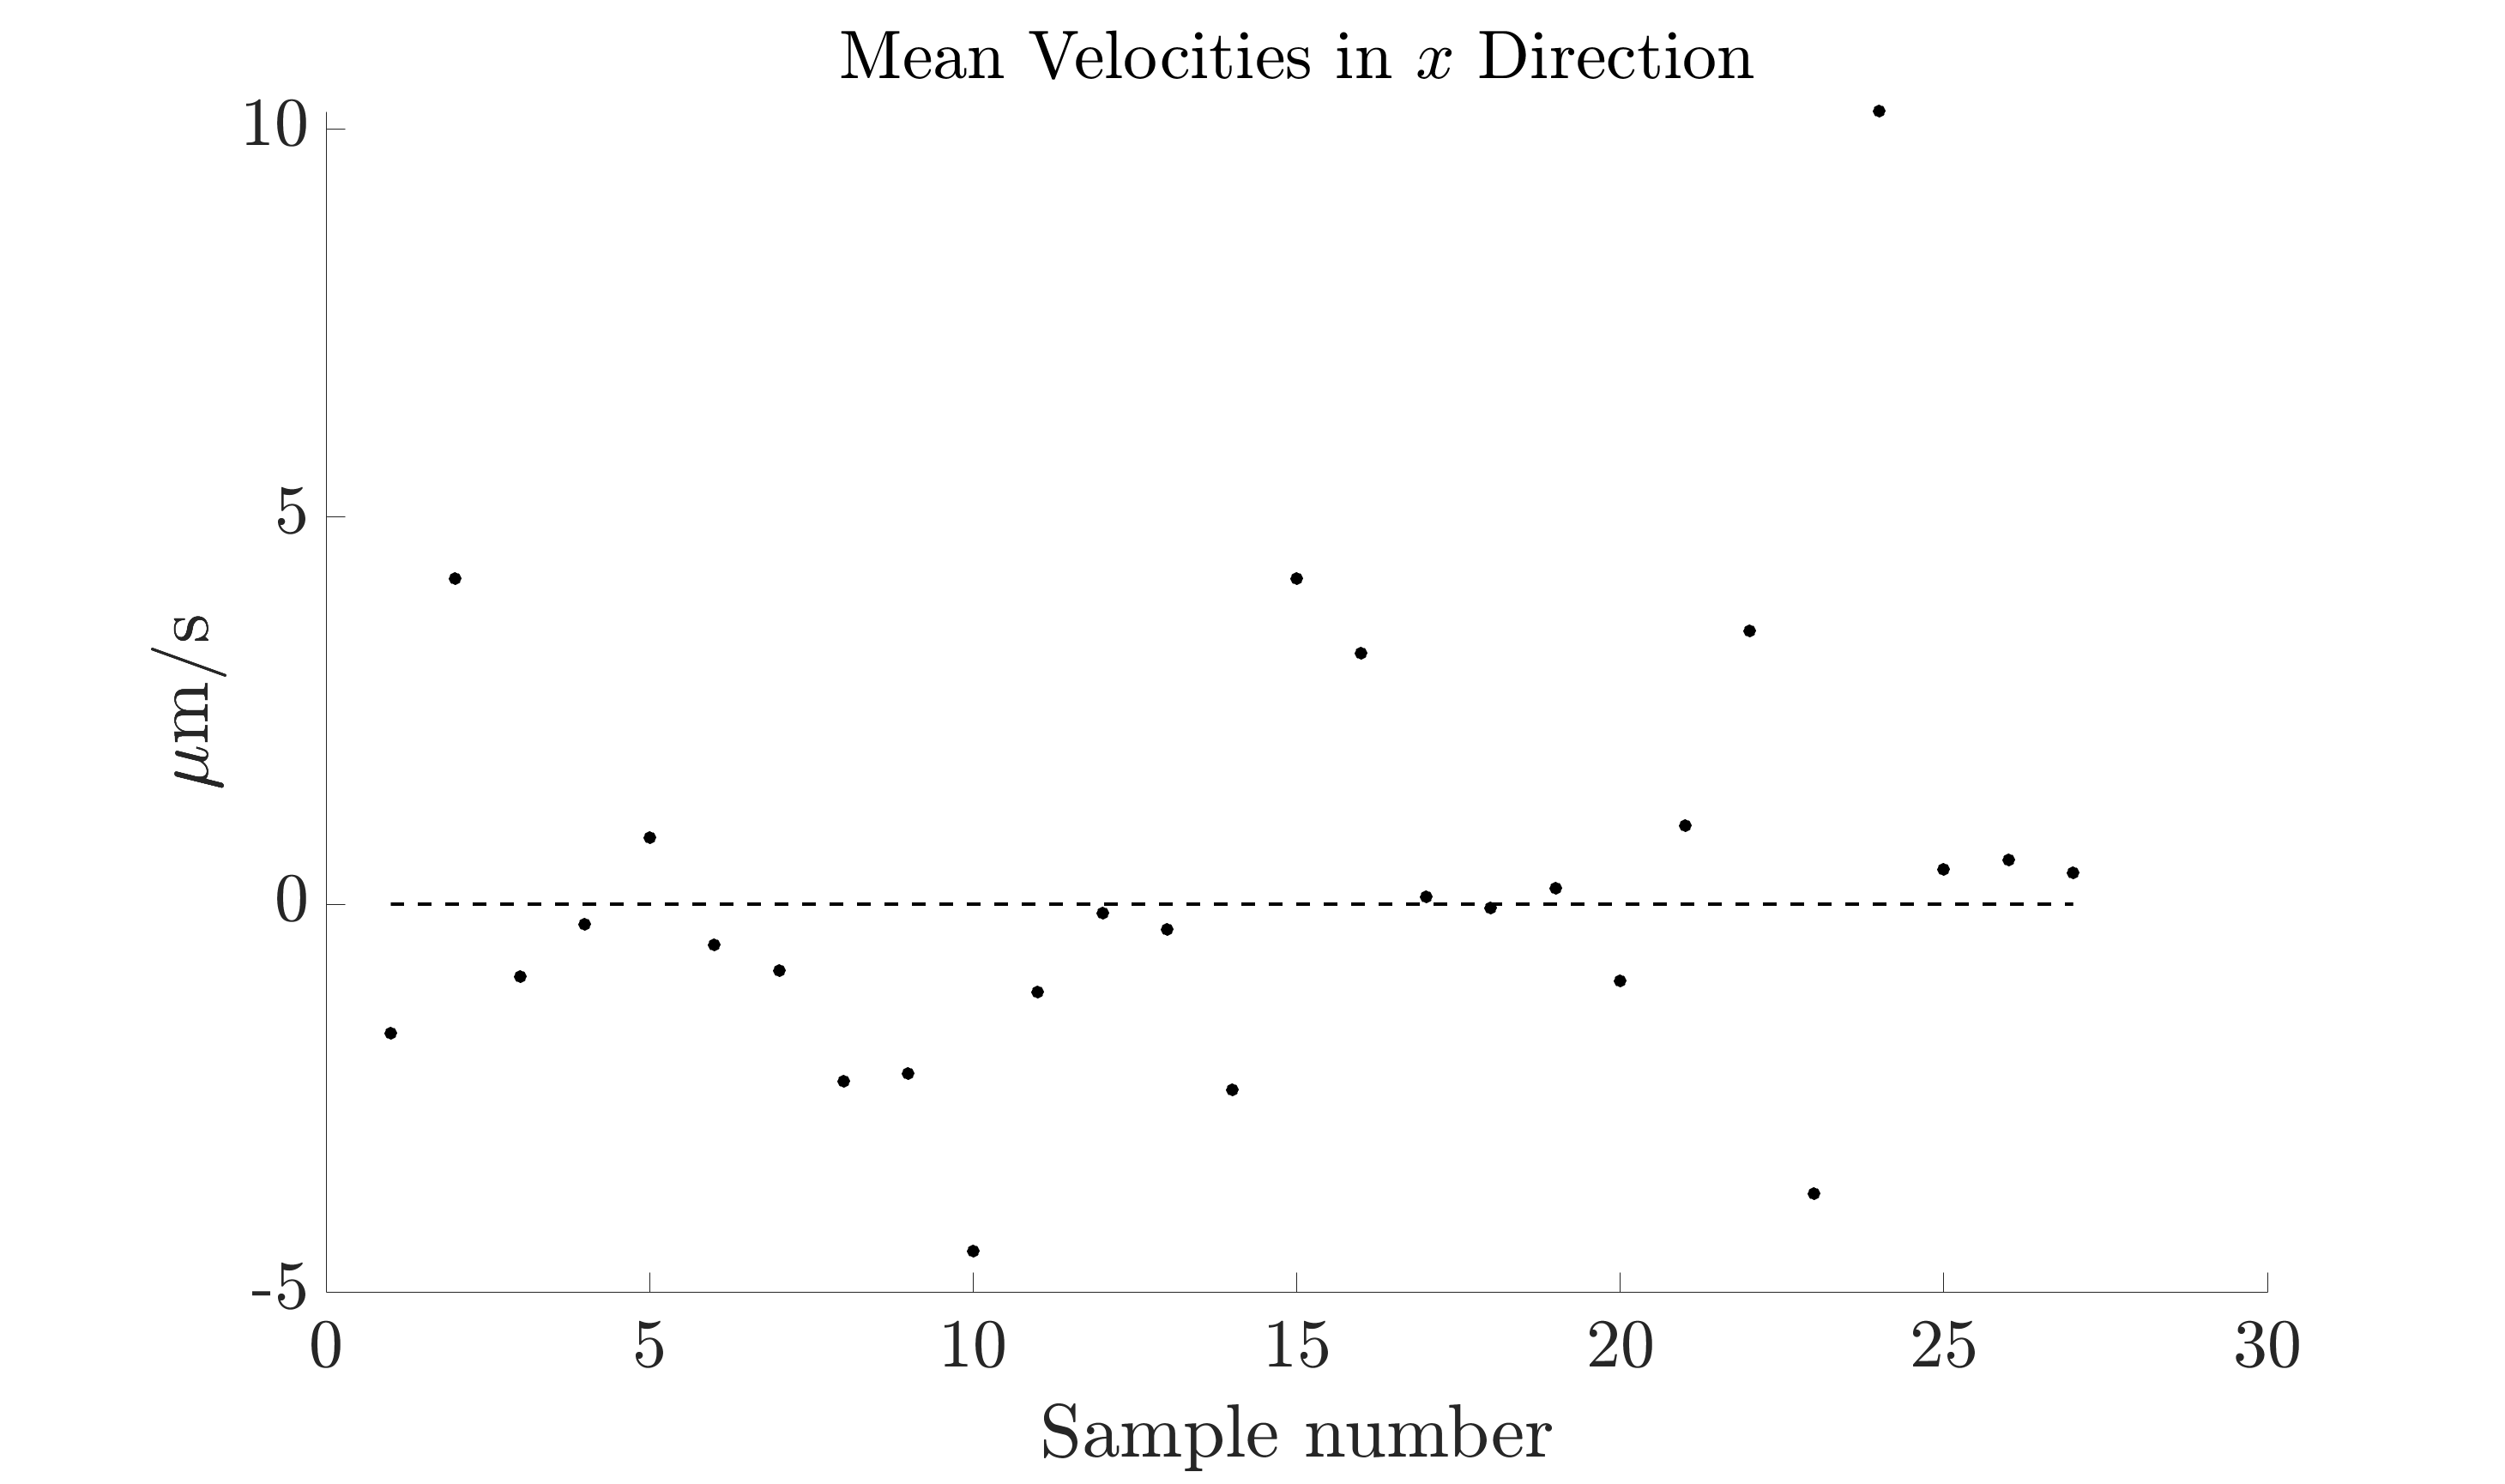
\includegraphics[width=\textwidth]{graphics/mean_velocities_x.png}
    \end{minipage}
    \begin{minipage}[t]{0.49\textwidth}
        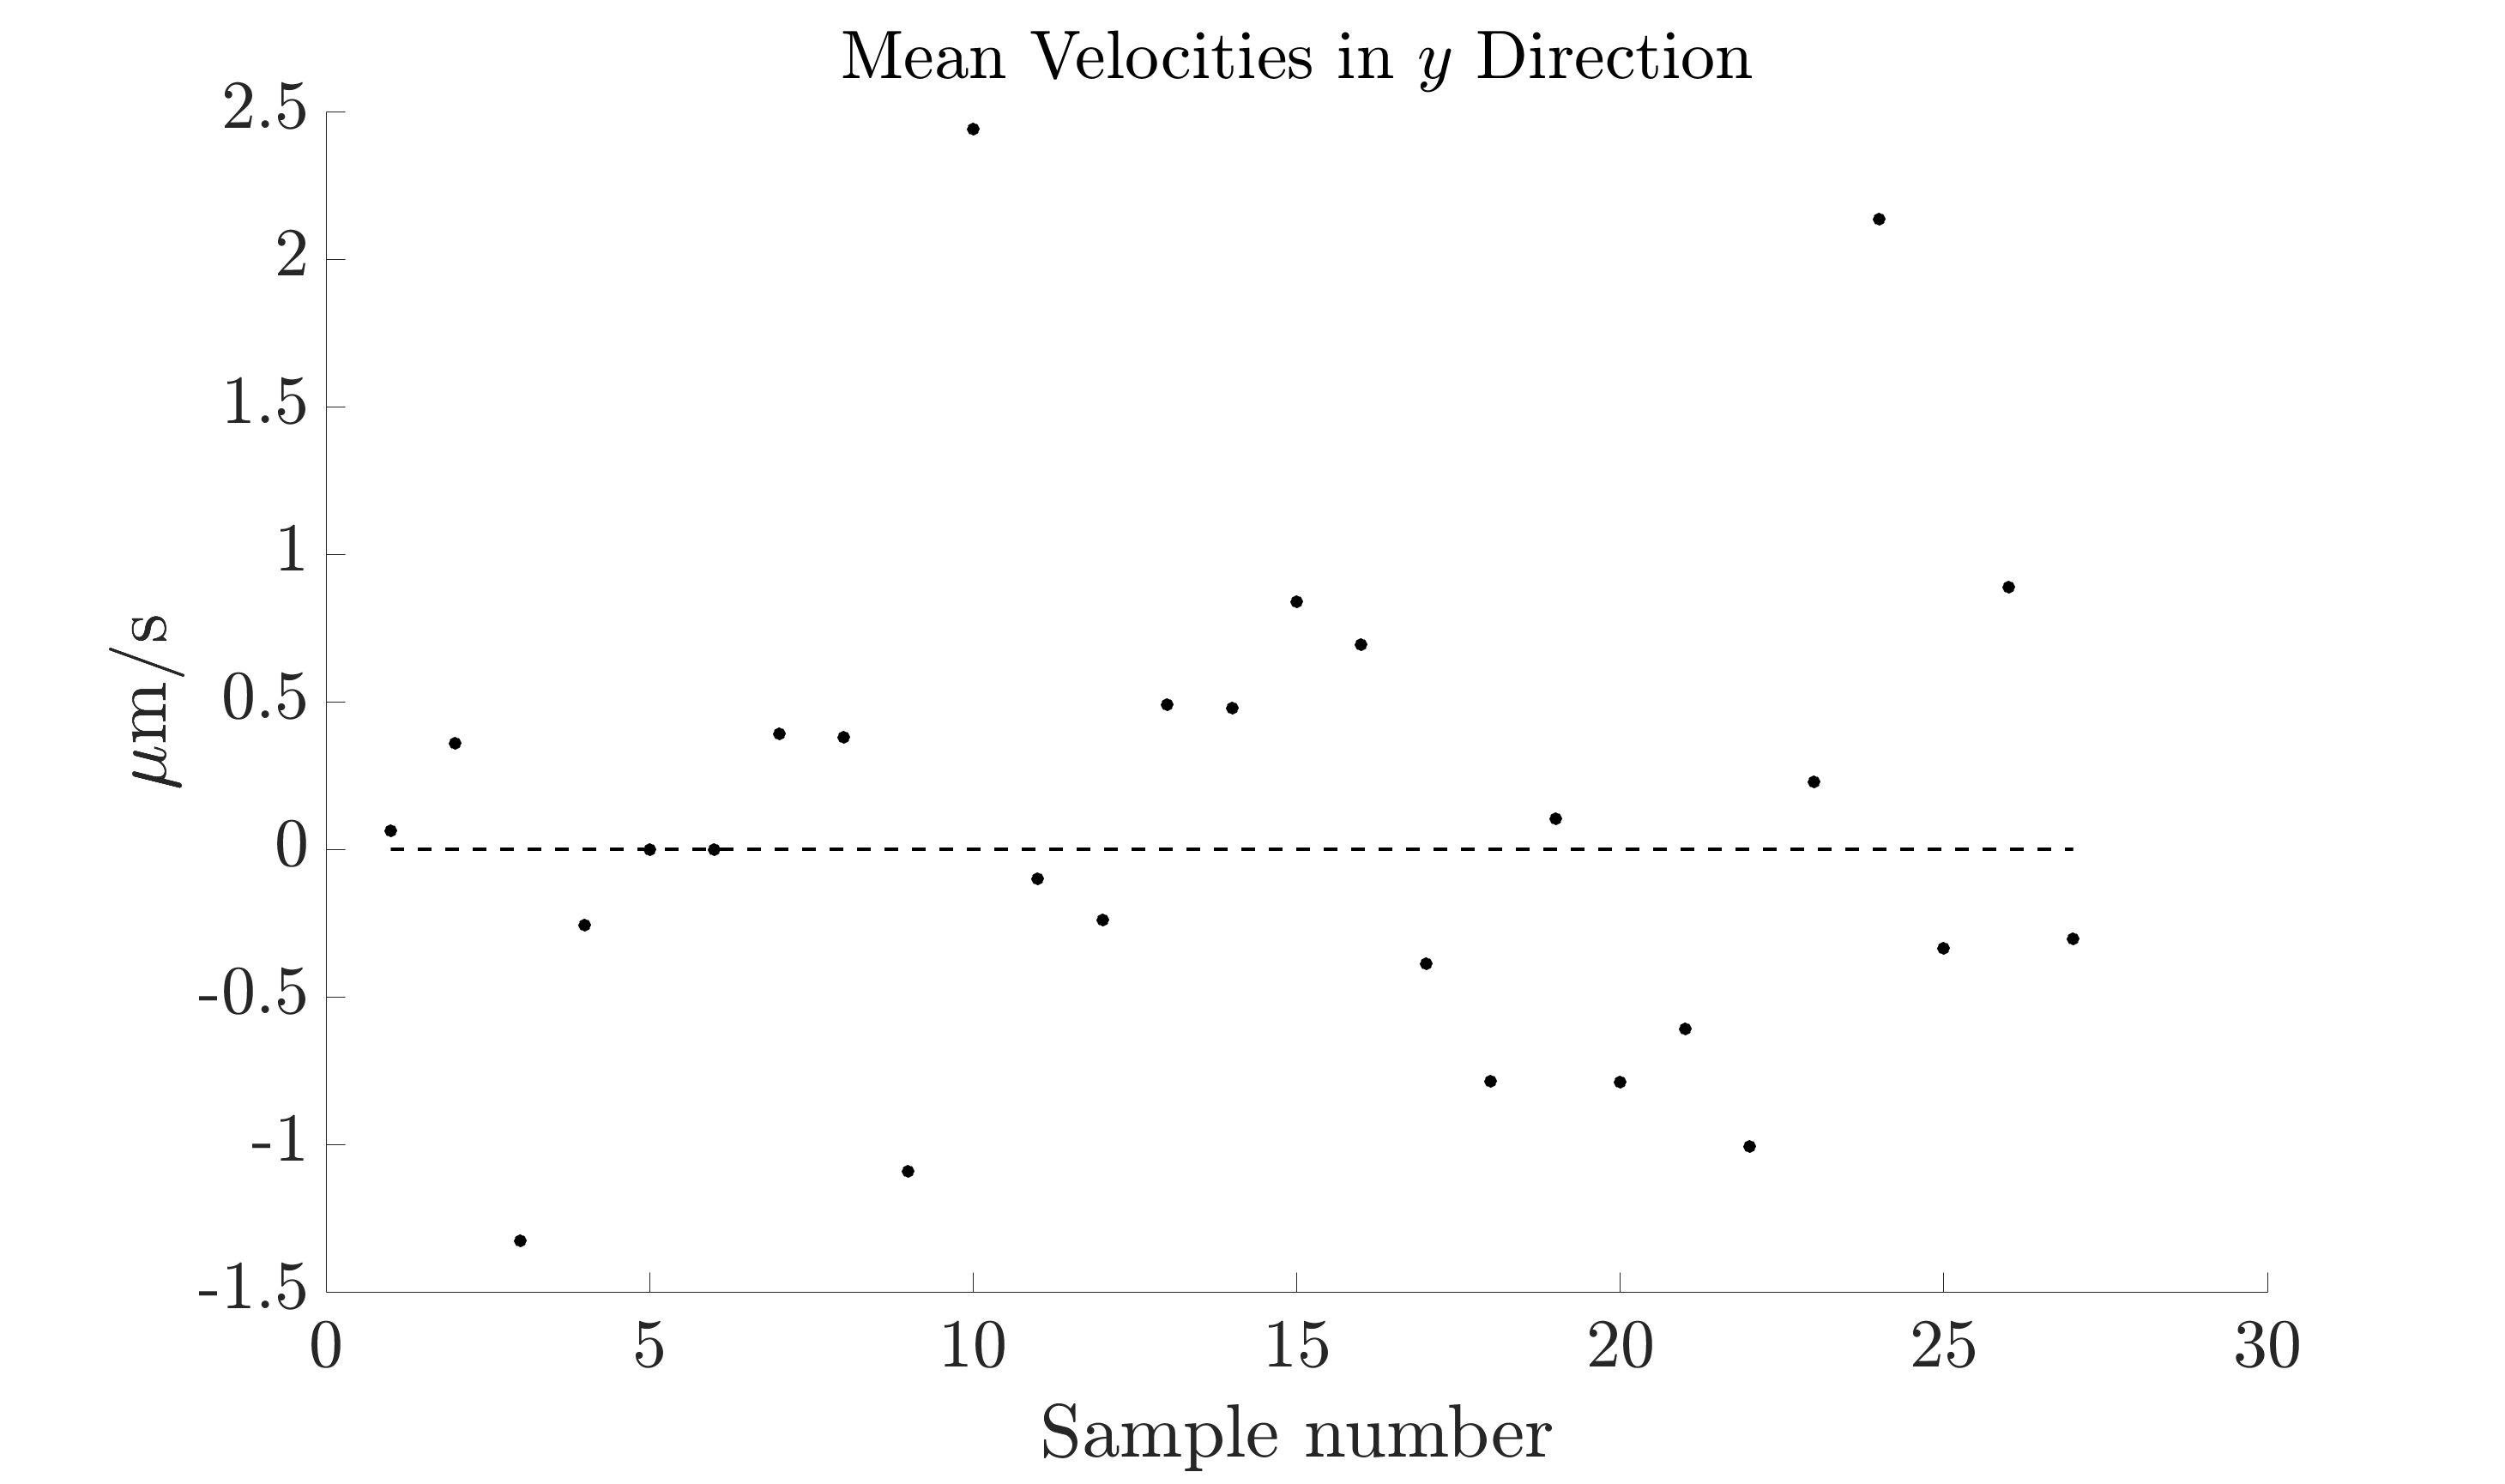
\includegraphics[width=\textwidth]{graphics/mean_velocities_y.png}
    \end{minipage} 
    \caption{Particle tracking data. Mean velocities in
    the $x$ (\textbf{a.}) and $y$ (\textbf{b.}) directions of the particles tracked.
    The dashed horizontal line designates a value of zero.}\label{fig:particle_tracking_data}
\end{figure}

\end{document}